\documentclass[12pt, twoside]{article}
\usepackage{amsmath, amssymb, amsthm}
\usepackage{bm, bbm}
\usepackage{algorithm}
\usepackage{algpseudocode}
\usepackage{float, graphicx, fullpage, parskip, subcaption, setspace, multicol}
\usepackage{comment}
\usepackage{url}
\usepackage{enumitem}
\usepackage{hyperref}
\usepackage{natbib}
\usepackage[usenames,dvipsnames]{xcolor}
\usepackage{nicematrix}
\usepackage{csquotes}
\usepackage{caption}

%
\captionsetup{belowskip=0pt}

% Define some colors
\definecolor{SkyBlue}{RGB}{14, 118, 188}
\definecolor{BrightRed}{RGB}{223, 82, 78}
\definecolor{Green638}{RGB}{165,255,118} % from colours.cafe on instagram; pallete638

% Set up colorful hyperlinks without any silly green boxes
\hypersetup{pdfborder = {0 0 0.5 [3 3]}, colorlinks = true, linkcolor = BrightRed, citecolor = SkyBlue}

\bibliographystyle{apalike}

% Math macros
\DeclareMathOperator*{\argmax}{arg\,max}
\DeclareMathOperator*{\argmin}{arg\,min}

\newcommand\numberthis{\addtocounter{equation}{1}\tag{\theequation}} % useful if we want to number one equation inside an align*
\newcommand\numbereqn{\addtocounter{equation}{1}\tag{\theequation}}

\newcommand{\R}{\mathbb{R}} % boldfaced R for the reals
\newcommand{\E}{\mathbb{E}} % boldfaced E for expectations
\def\P{\mathbb{P}} % boldfaced P for probability. overriding \P for paragraph symbol

\newcommand{\calP}{\mathcal{P}} % caligraphic P for a generic distribution
\newcommand{\calQ}{\mathcal{Q}} % caligraphic Q for another generic distribution
\newcommand{\calF}{\mathcal{F}} % caligraphic F, typically for sigma-algebras

\newcommand{\ind}[1]{\mathbbm{1}\left( #1 \right)} % indicator function, with an argument
\newcommand{\var}[1]{\textrm{Var}\left( #1 \right)} % variance
\newcommand{\cov}[2]{\textrm{Cov}\left( #1, #2 \right)} % covariance
\newcommand{\sign}[1]{\textrm{sign}\left(#1\right)} % sign
\newcommand{\parallelsum}{\mathbin{\|}} % for double bar to behave like a binary operation
\newcommand{\kl}[2]{\textrm{KL}\left(#1 \mid \parallelsum \# \right)} % KL divergence with two arguments


% distributions
\newcommand{\normaldist}[2]{\mathcal{N}\left(#1,~#2\right)} % normal distribution
\newcommand{\mvnormaldist}[3]{\mathcal{N}_{#1}\left(#2,~#3\right)} % multivariate normal distribution
\newcommand{\gammadist}[2]{\textrm{Gamma}\left(#1,~#2\right)} % gamma distribution
\newcommand{\igammadist}[2]{\textrm{Inv.~Gamma}\left(#1,~#2\right)} % inverse gamma
\newcommand{\binomialdist}[2]{\textrm{Binomial}\left(#1,~#2\right)} % Binomial
\newcommand{\berndist}[1]{\textrm{Bernoulli}\left(#1\right)} % Bernoulli
\newcommand{\poisdist}[1]{\textrm{Poisson}\left(#1\right)} % Poisson
\newcommand{\hafltdist}[2]{\textrm{half-t}_{\#1}\left(#2\right)} %half-t
\newcommand{\unifdist}[2]{\textrm{Uniform}\left(#1,~#2\right)} % uniform
\newcommand{\betadist}[2]{\textrm{Beta}\left(#1,~#2\right)} % Beta distribution

% bolded alphabet time
\newcommand{\by}{\bm{y}}
\newcommand{\bx}{\bm{x}}
\newcommand{\bz}{\bm{z}}
\newcommand{\bw}{\bm{w}}

% bolded capitalized alphabet
\newcommand{\bY}{\bm{Y}}
\newcommand{\bX}{\bm{X}}

% bolded greek alphabet time!
\newcommand{\btheta}{\boldsymbol{\theta}}
\newcommand{\bbeta}{\boldsymbol{\beta}}

%overline time
\newcommand{\ybar}{\overline{y}}
\newcommand{\xbar}{\overline{x}}
\newcommand{\mubar}{\overline{\mu}}

% for maximal laziness, anytime we need to refer to a generic prior, posterior, joint, or marginal density, we can use the follwing
\newcommand{\prior}{p(\theta)}
\newcommand{\like}{p(\by \vert \theta)}
\newcommand{\marg}{p(\by)}
\newcommand{\joint}{p(\by,\theta)}
\newcommand{\post}{p(\theta \vert \by)}

% Theorem-like declarations
\theoremstyle{plain}
\newtheorem{theorem}{Theorem}
\newtheorem{corollary}[theorem]{Corollary}
\newtheorem{lemma}[theorem]{Lemma}
\newtheorem{proposition}[theorem]{Proposition}

\theoremstyle{definition}
\newtheorem{definition}[theorem]{Definition}

\newtheorem{ex}{Example}
\newenvironment{example}{\begin{ex}}{ \hfill $\blacksquare$\end{ex}}


\theoremstyle{remark}
\newtheorem{remark}[theorem]{Remark}

% comment fields
\newcommand{\skd}[1]{\textcolor{red}{[skd]: #1}} % includes all of the macros and sets default layout and formating

\title{A Bayesian Hierarchical Model \\ For Predicting Song Popularity\footnote{Data and code are available on \href{https://github.com/james-hubbs/A-Bayesian-Hierarchical-Model-For-Predicting-Song-Popularity}{GitHub}}}
\author{James Hubbs}
\begin{document}
\onehalfspacing % don't change the spacing
\maketitle

\section{Introduction}
I consider the question of predicting song popularity. What is it that makes certain songs popular? There are seemingly infinitely many possible factors. Of primary interest here, however, is whether or not the particular \textit{audio} qualities of a song are predictive of its popularity. Do things like tempo, rhythm, timbre, and other qualities of the sound help drive popularity?

One might initially assume this to be obviously true. Popular songs tend to leverage a predictable set of tools---most popular songs are in common time and use similar harmonic structures, for example. So rather than analyzing audio features and popularity across all styles of music, I instead focus entirely on songs within the popular framework. Among these songs, can popularity be accurately predicted using features of the audio? 

Although pop songs often share some similarities, there remains lots of variation to analyze. For example, Billboard's Year-End Hot 100 Songs chart for 2021\footnote{\href{https://www.billboard.com/charts/year-end/hot-100-songs/}{https://www.billboard.com/charts/year-end/hot-100-songs/}} features ``Leave The Door Open" by Silk Sonic, a soulful callback to late 70s R\&B, and ``Levitating" by Dua Lipa, a hypermodern electronic dance track. Further, I consider 51 years of popular music beginning in 1970 and ending in 2021---of course, there are large stylistic differences across time. 

In this analysis, I show that among select pop songs from 1970-2021, audio features are at best weakly predictive of song popularity. 
% I also find evidence that danceability---a measure of how suitable a song is for dancing---is most predictive of popularity.

\section{Data Description and Exploration}
I consider data from Spotify's Web API. Spotify is one of the largest music streaming services in the world. They're known for their data-forward approach toward streaming---the service makes extensive use of machine learning-based recommendation algorithms, which of course require considerable amounts of data. Some of this data is made available publicly through their web API.\footnote{Documentation is available at \href{https://developer.spotify.com/documentation/web-api/}{https://developer.spotify.com/documentation/web-api/}}

The data were sampled in March 2022. For each year between 1970 and 2021, the Spotify-generated playlists for top hits within a given year were used\footnote{For example, ``Top Hits of 2000": \href{https://open.spotify.com/playlist/37i9dQZF1DWUZv12GM5cFk}{https://open.spotify.com/playlist/37i9dQZF1DWUZv12GM5cFk}}. Using the top hits playlists ensures that our scope is narrowed to songs within the popular framework. It's also a convenient way to acquire a sample of music from each year in consideration. Each playlist consists of approximately $100$ songs, so across 51 years we have a total sample size of about $5,100$.

\subsection{Audio Features and Popularity}
The following table provides summarized definitions of the primary predictors in consideration. The response variable is popularity, which Spotify describes somewhat vaguely as ``The popularity is calculated by algorithm and is based, in the most part, on the total number of plays the track has had and how recent those plays are." The specifics of this algorithm are not described in their documentation. An important implication here is that we are analyzing \textit{current} popularity. That is, we are not analyzing historical popularity of songs, but rather their popularity at the time of sampling in March 2022.

As with popularity, the below predictors are not defined by Spotify in great detail:

\begin{table}[H]
\centering
\caption{Definitions of audio feature predictors}
\label{tab:results}
\def\arraystretch{1.5}
\begin{tabular}{l  p{10cm}  p{3.4cm}} % note the 
\hline
Variable & Spotify Definition (Summarized) \\ \hline
acousticness & A confidence measure from 0.0 to 1.0 of whether the track is acoustic. \\
danceability & Danceability describes how suitable a track is for dancing based on a combination of musical elements including tempo, rhythm stability, beat strength, and overall regularity. \\
duration\_ms & The duration of the track in milliseconds. \\
instrumentalness & Predicts whether a track contains no vocals. \\
liveness & Detects the presence of an audience in the recording. \\
loudness & The overall loudness of a track in decibels (dB). \\
speechiness & Speechiness detects the presence of spoken words in a track. \\
tempo & The overall estimated tempo of a track in beats per minute (BPM). \\
valence & A measure from 0.0 to 1.0 describing the musical positiveness conveyed by a track. 
\end{tabular}
\end{table}
Despite a lack of detail surrounding how these features are constructed by Spotify, it is generally easy to understand them intuitively. For example, Billie Eilish's ``Your Power," a soft acoustic folk ballad that essentially uses only voice and acoustic guitar, is one of the highest scoring ``acousticness" songs in the entire dataset. 

\subsection{Hierarchical Nature of the Data}
Songs within a certain period of time are likely to be correlated. Popular songs that were released in the 1970s, for instance, often share some characteristics. The same is true for other time periods. Similarly, since we are measuring present popularity of songs, rather than historic popularity, it may be the case that a listener's relationship with audio features could vary by time period. A listener may enjoy ``danceable" songs from the 1980s, but generally dislike more modern songs that score high in danceability (the converse, of course, may also be true for other listeners). It's for these reasons that I view the data through a hierarchical lens, using release decade as the grouping variable. In principle, a more narrow grouping (e.g., by year) could be employed. Though music is often conceptualized in a decade-by-decade fashion, so decade is a natural choice for grouping the data.

\subsection{Exploration}
There is much to be learned about this dataset through visualization.

The below figure summarizes popularity by decade. Of course, popularity tends to be greater in more recent decades. This is simply reflective of the fact that we're measuring present popularity. In turn, it may also reflect Spotify's user demographics, since over 50\% of Spotify users are under the age of 34\footnote{\href{https://www.businessofapps.com/data/spotify-statistics/}{https://www.businessofapps.com/data/spotify-statistics/}}, and younger users will likely prefer newer songs. We also see that across all decades, the median popularity is greater than 50, and this is a product of having sampled generally popular songs, since songs were selected via the ``top hits" playlists. Finally, we observe there are many low-valued outliers within each decade---these observations will later prove particularly difficult to predict.

\begin{figure}[H] % H forces the figure to appear in this location, h! tries really hard to do the same thing
\centering
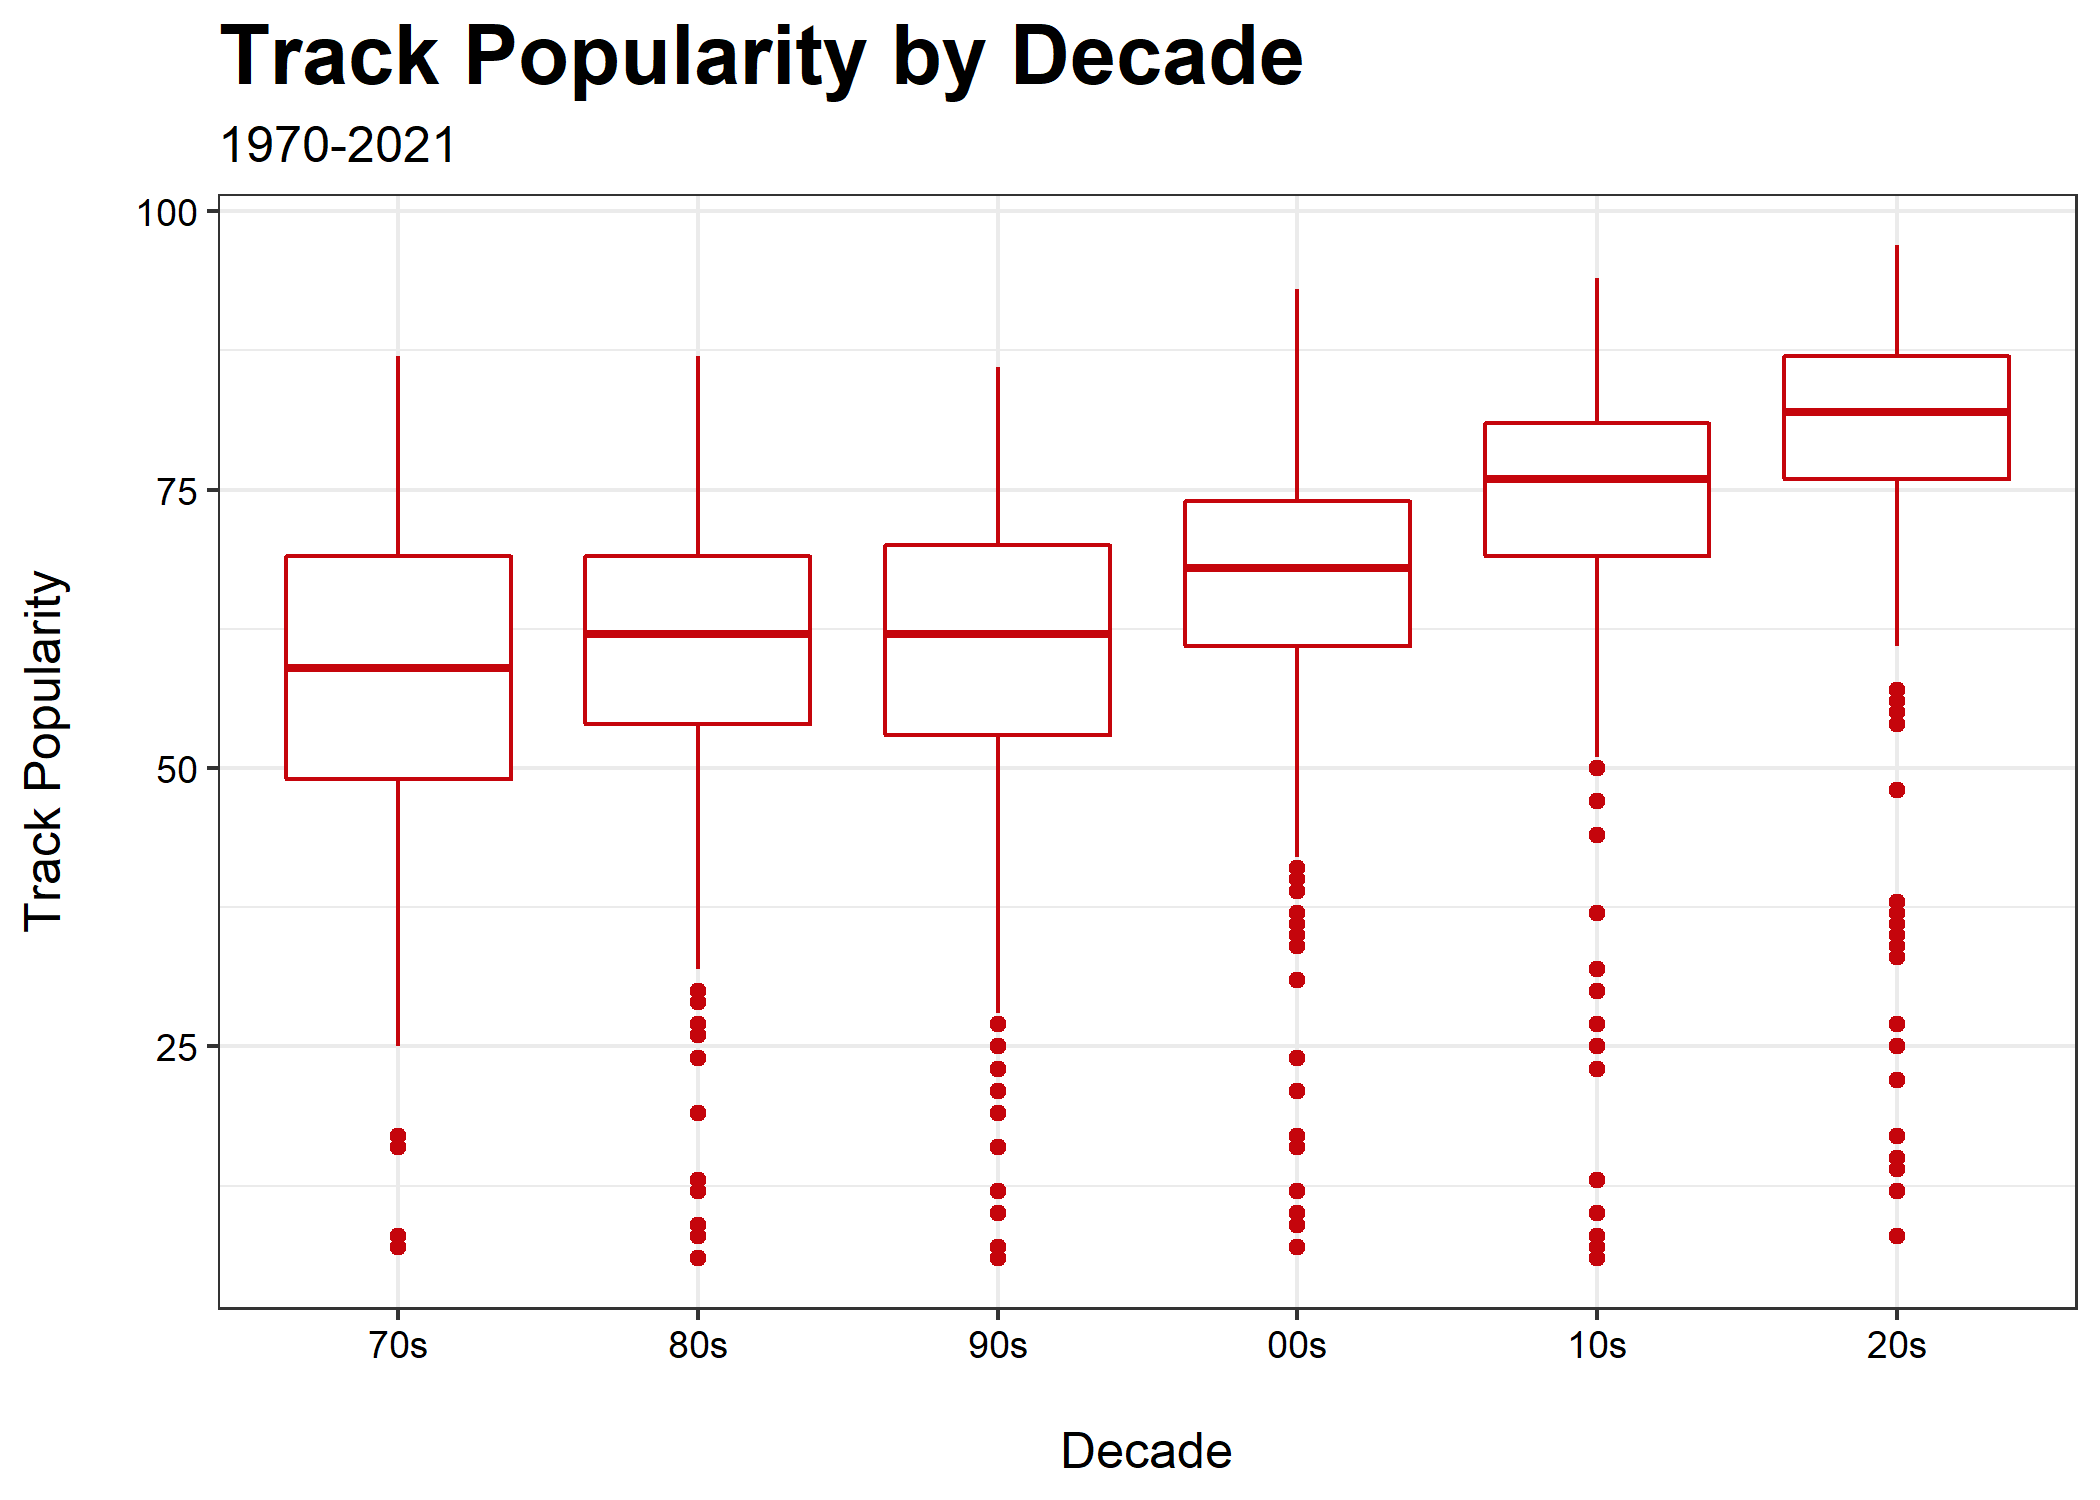
\includegraphics[width=0.7\textwidth]{track_pop_decade.png} % no need to specify a file extension & pay attention to scaling by width!
\caption{Track popularity over time. Since popularity is measuring present popularity, songs from more recent time periods have greater popularity. Note that ``20's" includes only 2020 and 2021.}
\label{fig:track_pop_decade} % useful for hyperref'ing later
\end{figure}

There are other interesting temporal features of this dataset. In particular, there are prominent trends among some of the predictors:

\begin{figure}[H]
\begin{subfigure}[b]{0.5\textwidth}
\centering
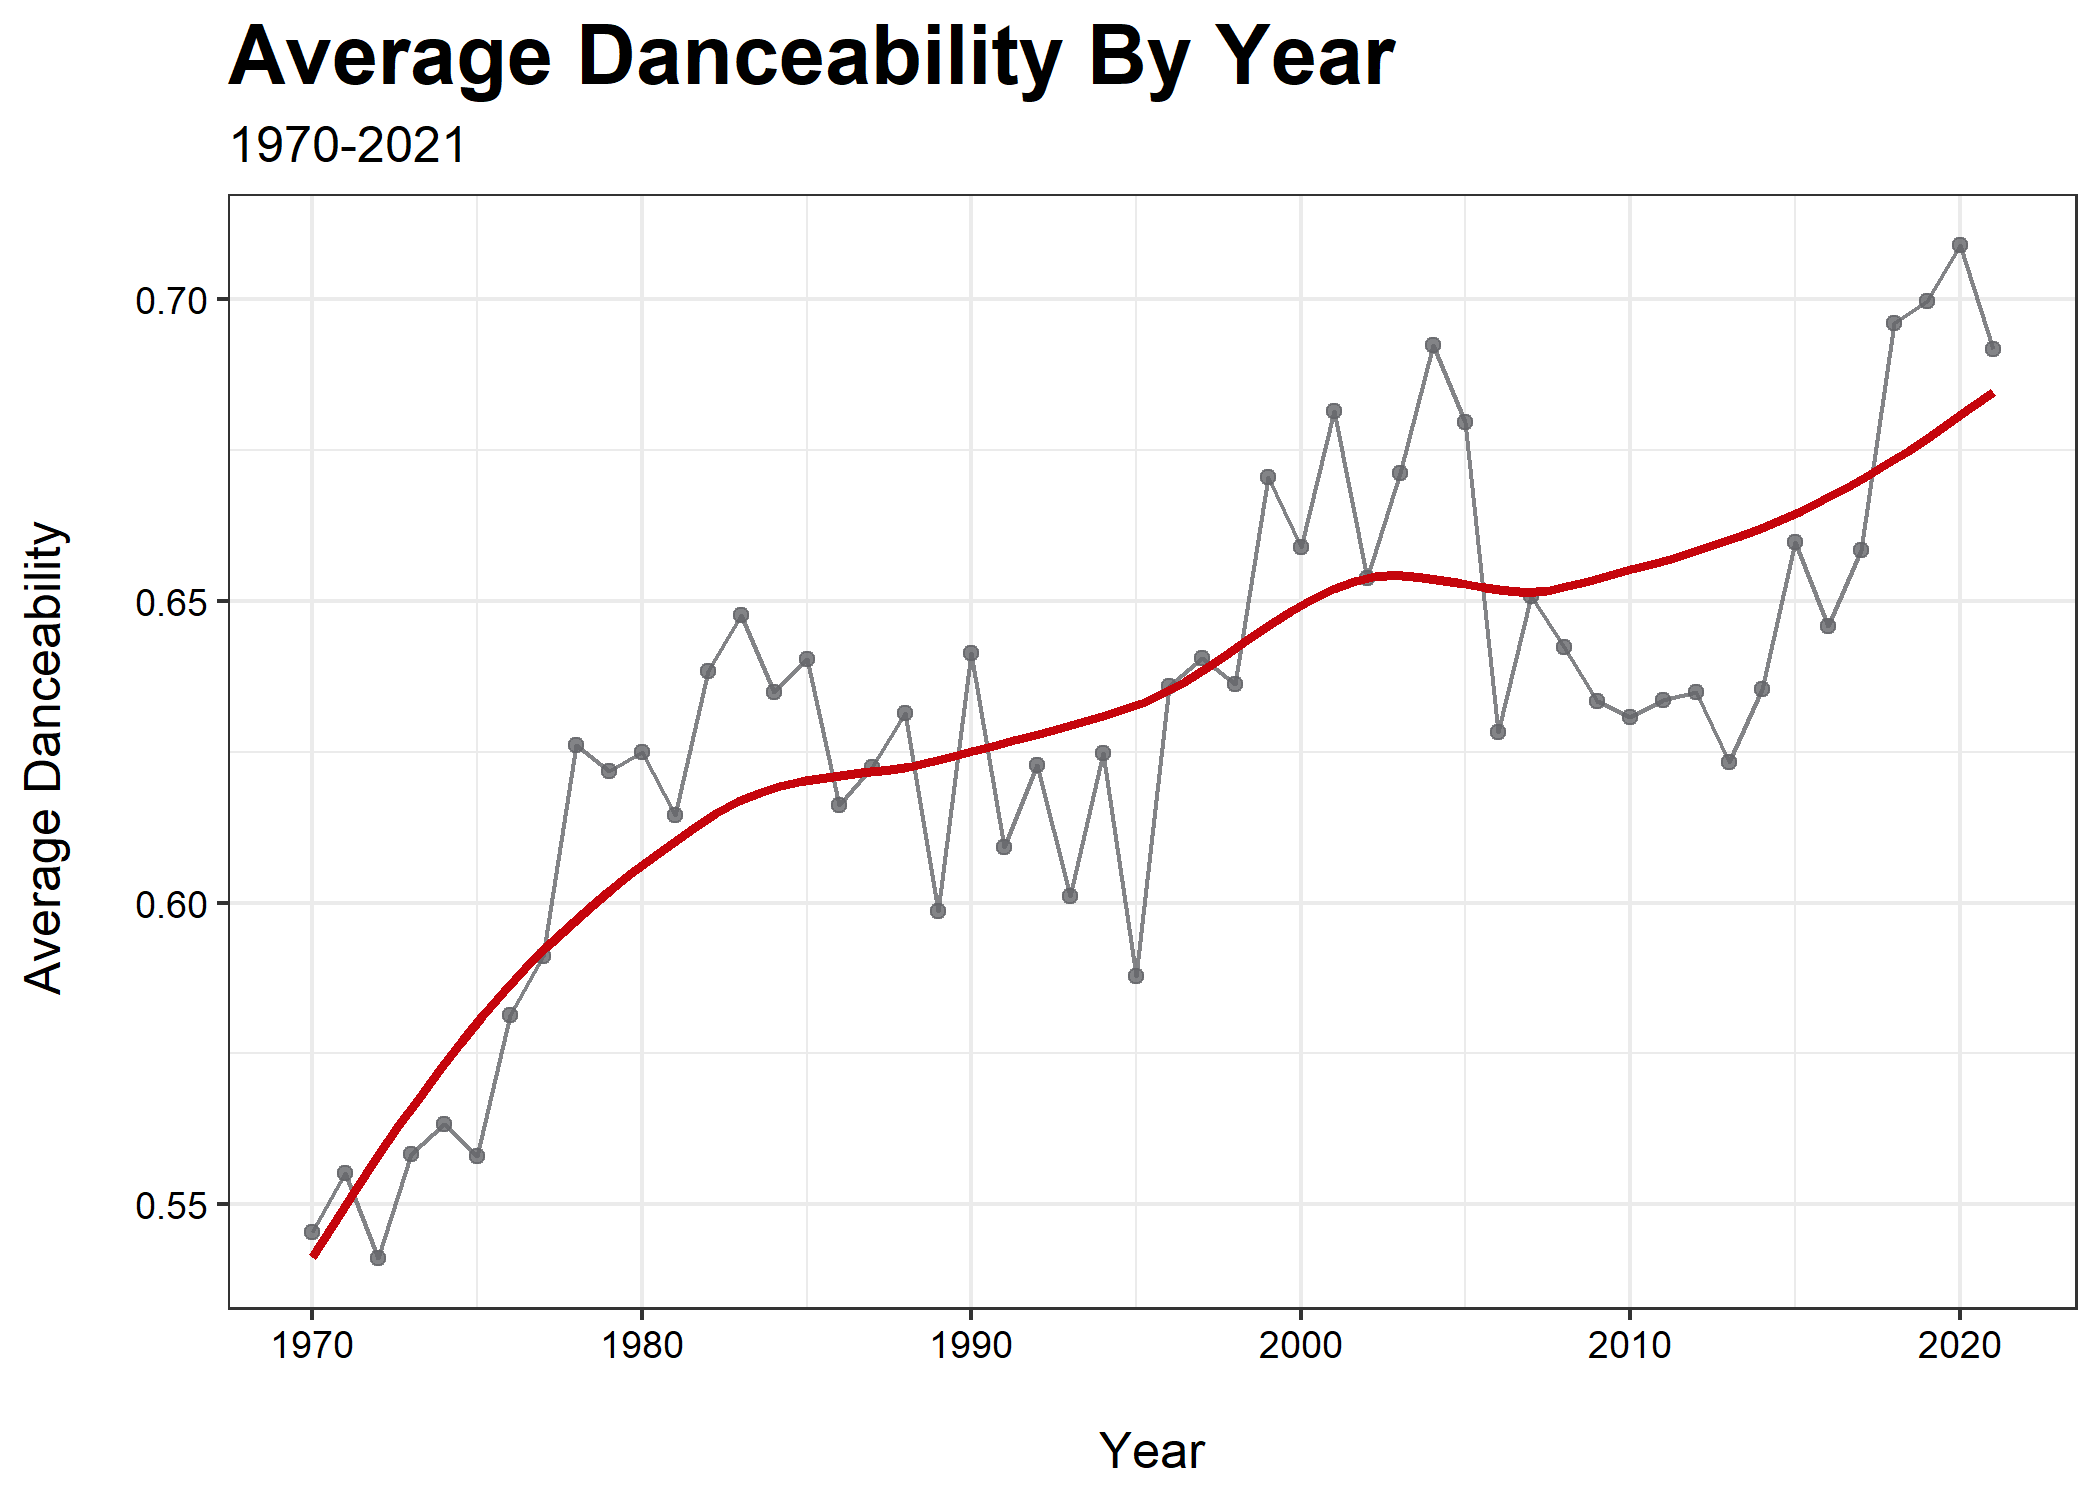
\includegraphics[width = \textwidth]{track_danceability_trend_.png}
\caption{}
\label{fig:danceability_trend}
\end{subfigure}
\begin{subfigure}[b]{0.5\textwidth}
\centering
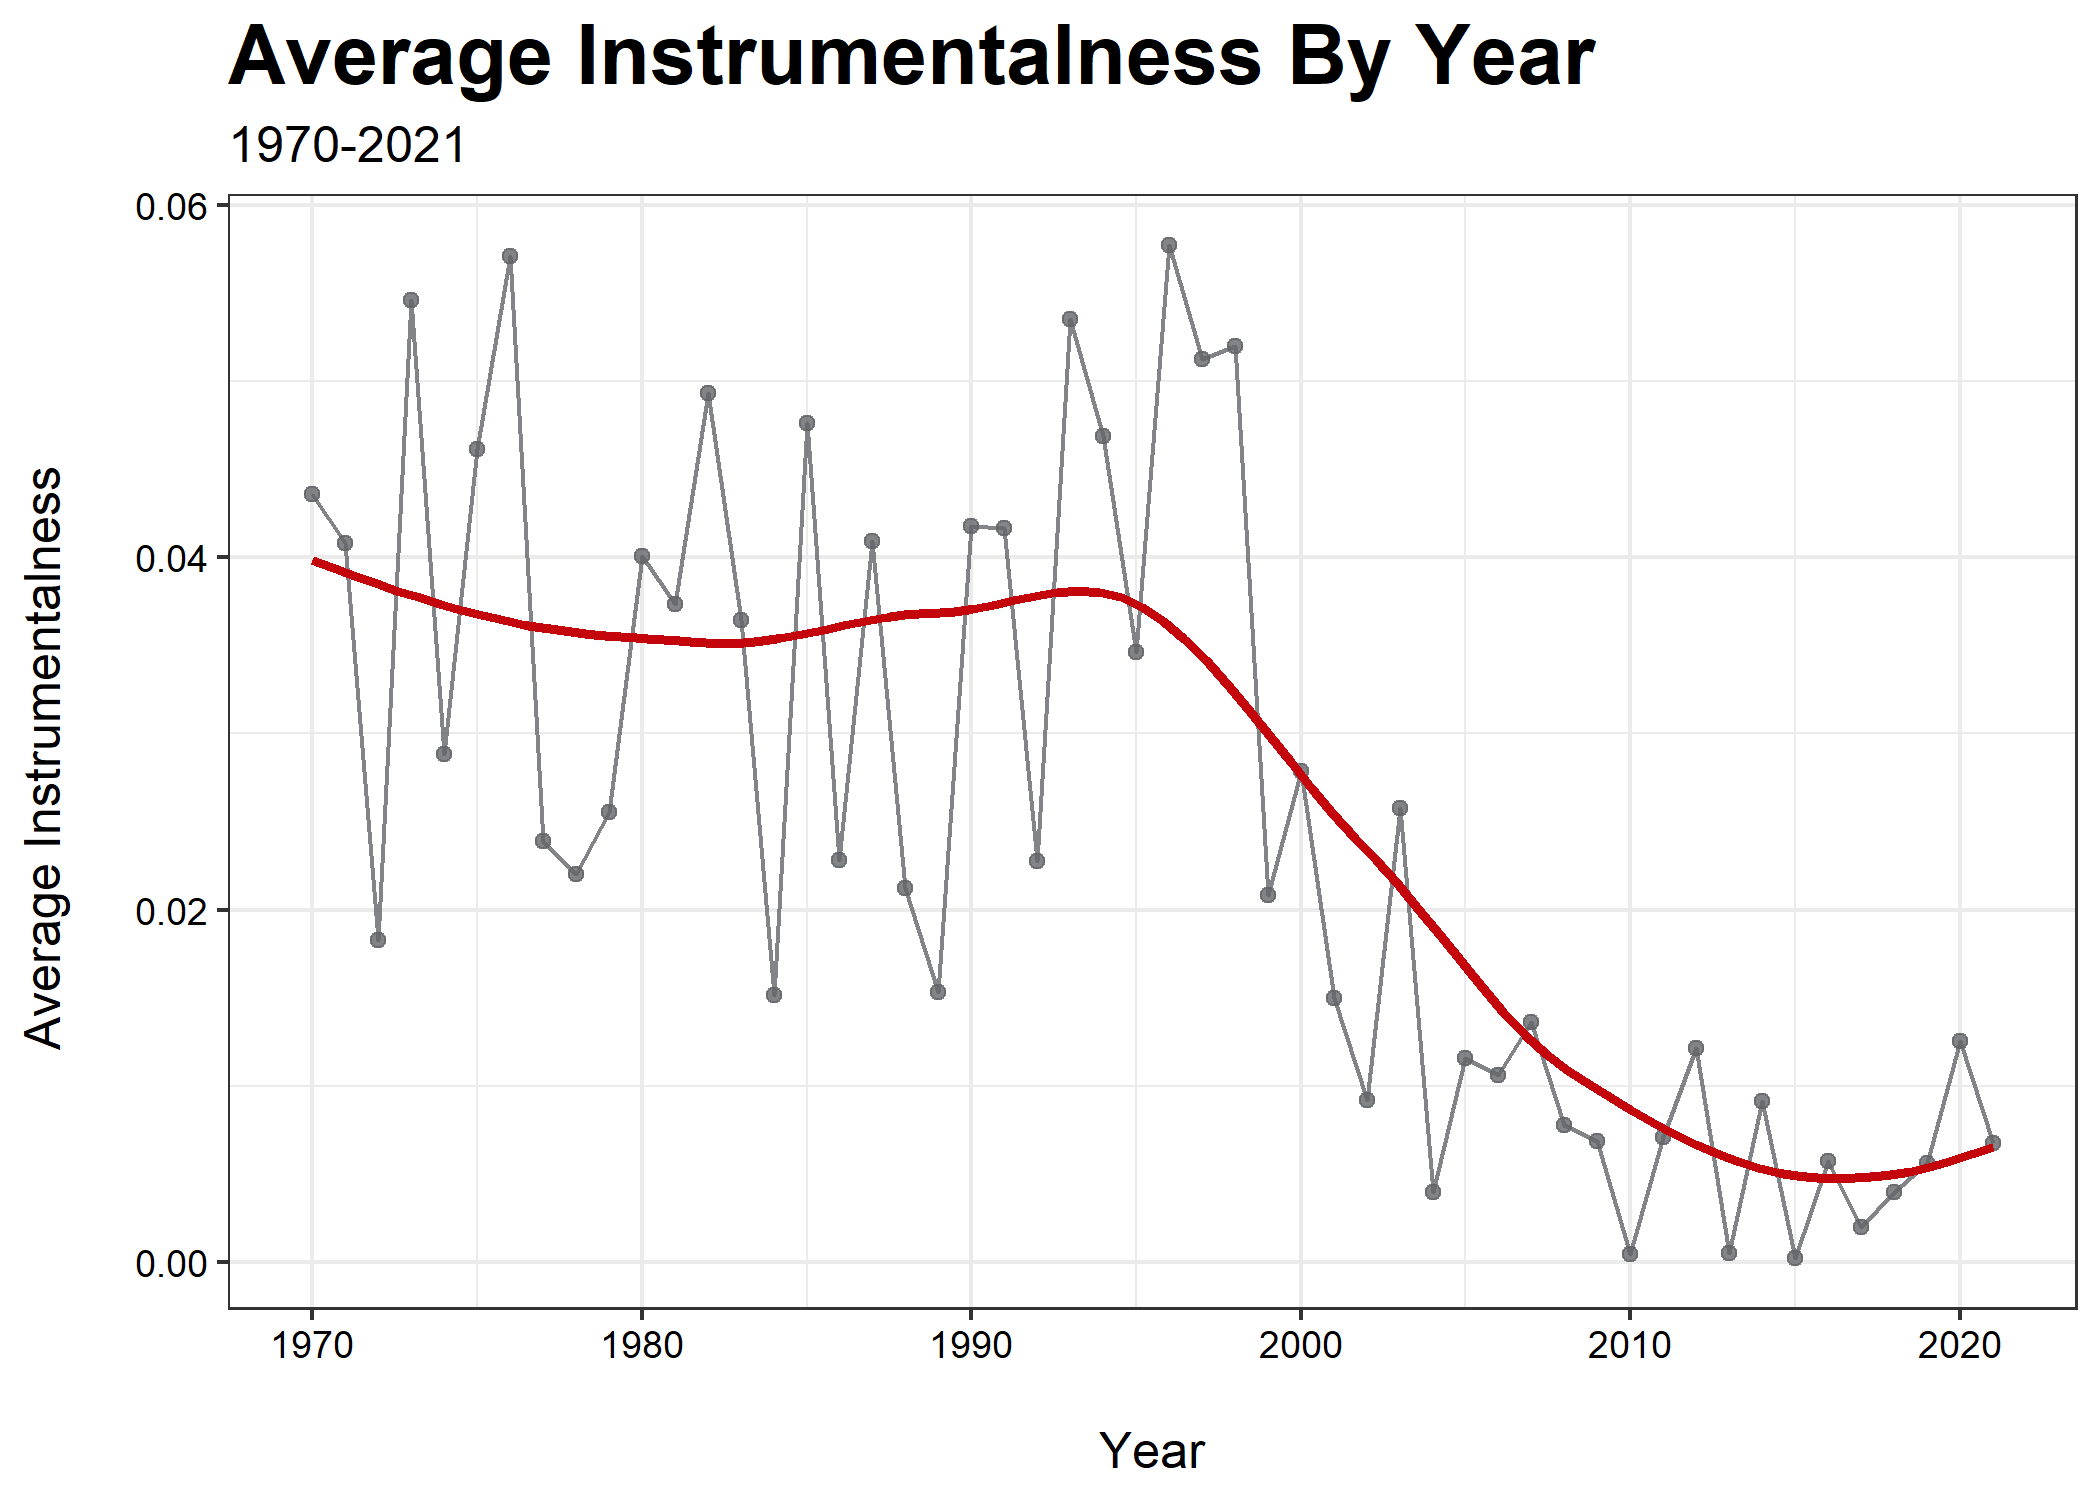
\includegraphics[width = \textwidth]{track_instrumentalness_trend_.png}
\caption{}
\label{fig:instrumentalness_trend}
\end{subfigure}
\begin{subfigure}[b]{0.5\textwidth}
\centering
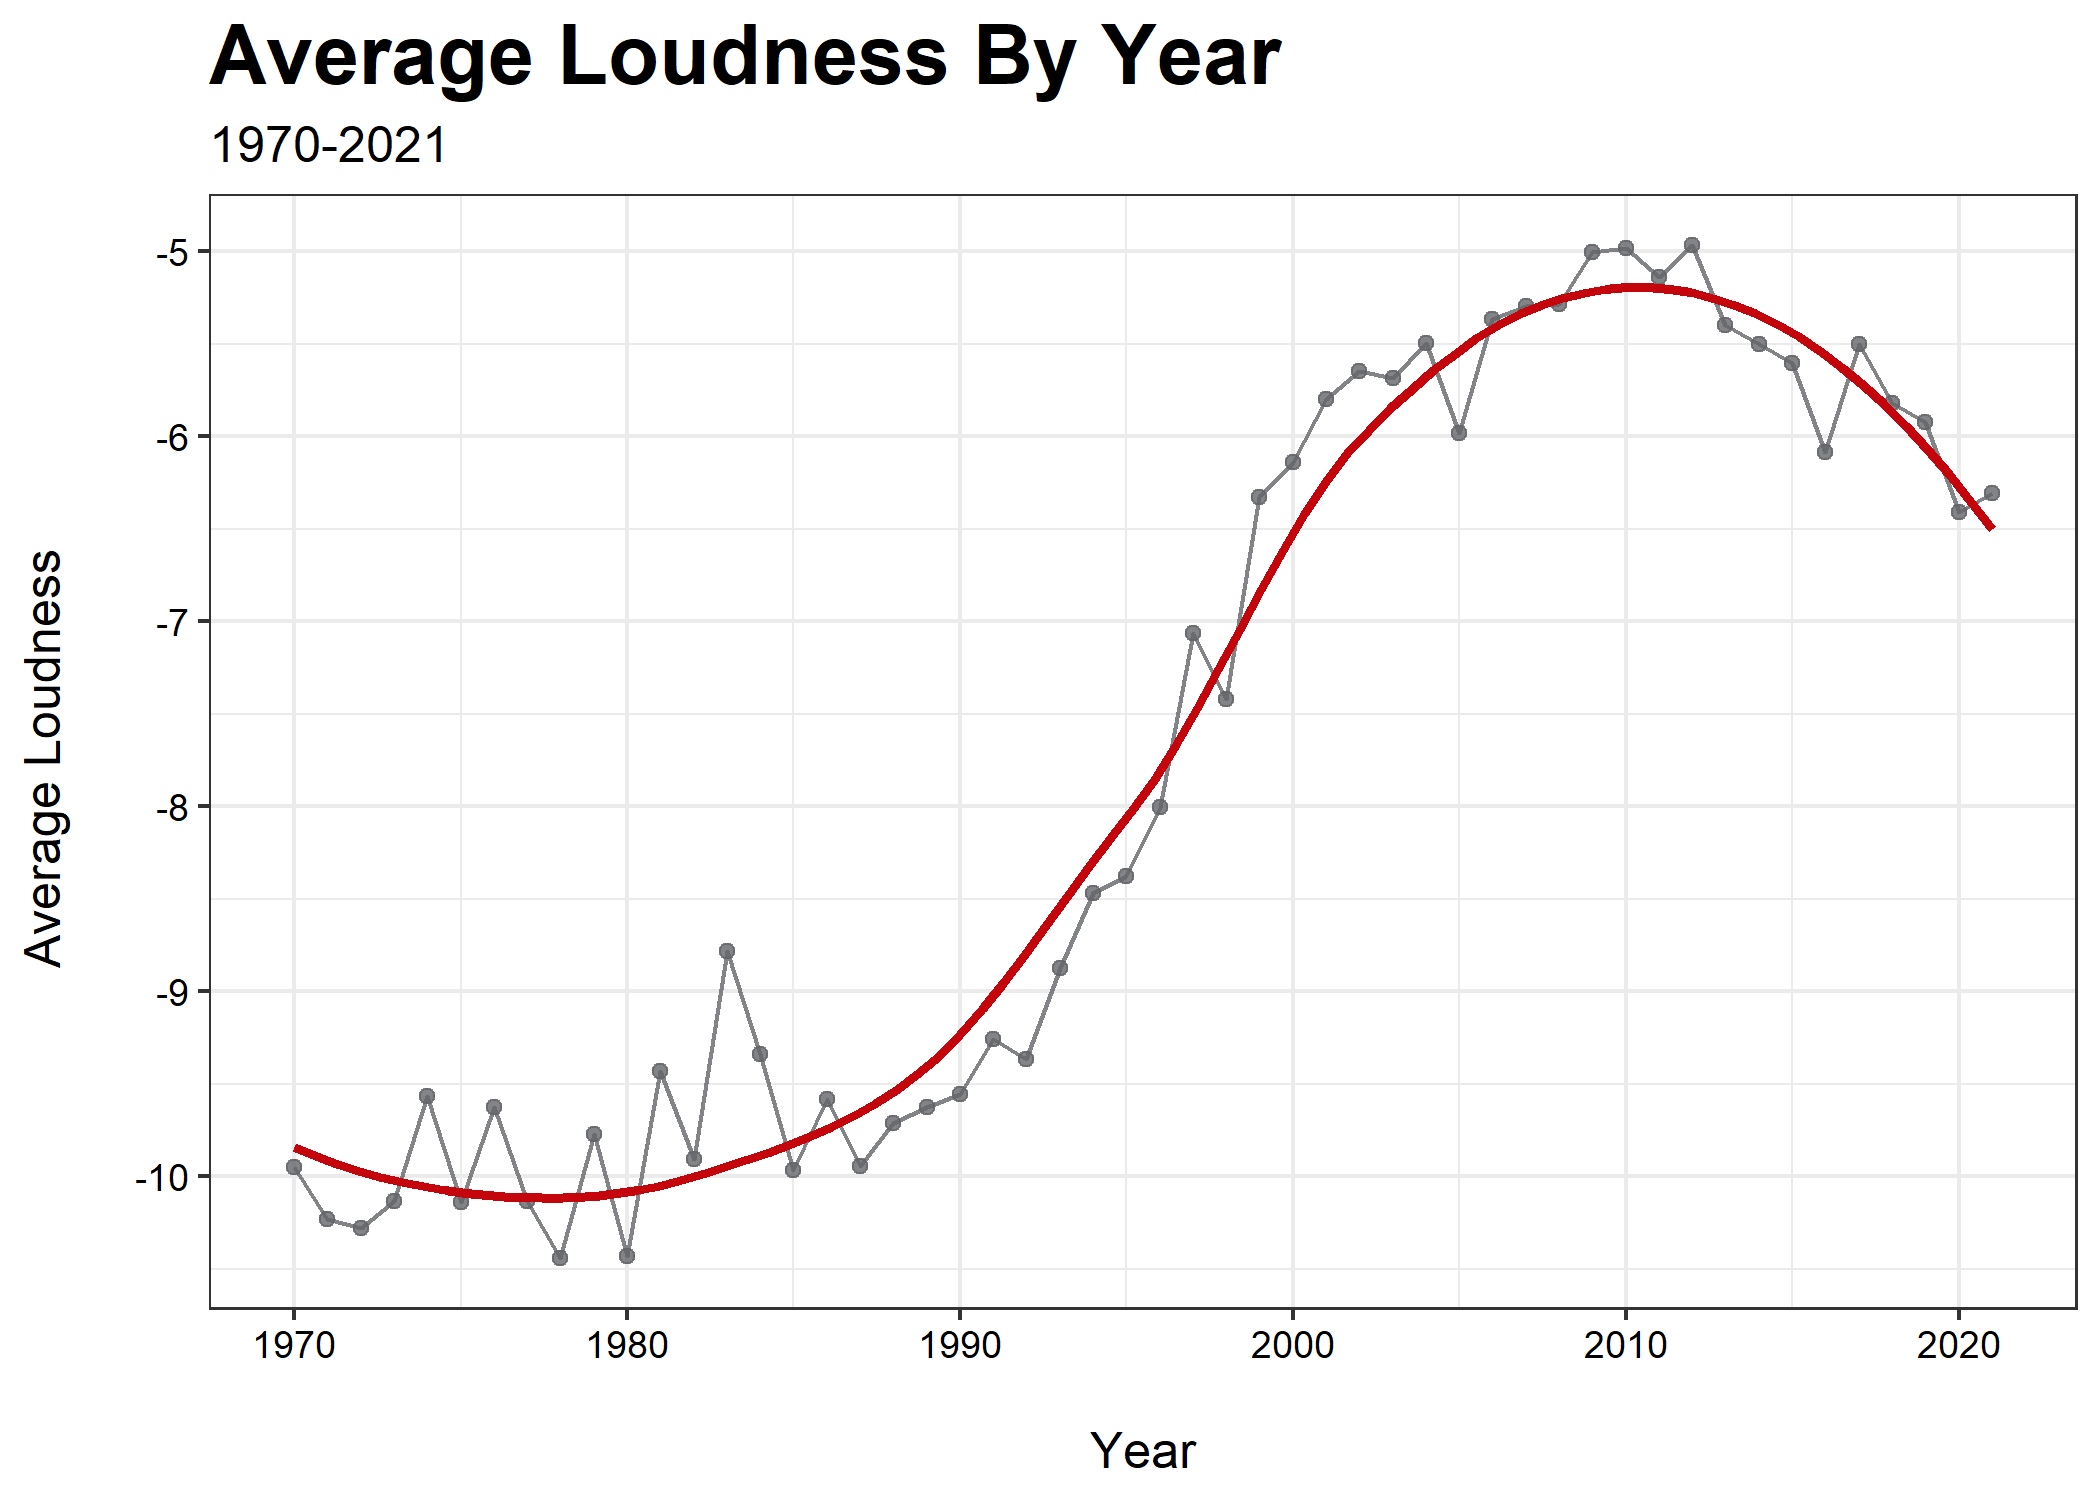
\includegraphics[width = \textwidth]{track_loudness_trend_.png}
\caption{}
\label{fig:loudness_trend}
\end{subfigure}
\begin{subfigure}[b]{0.5\textwidth}
\centering
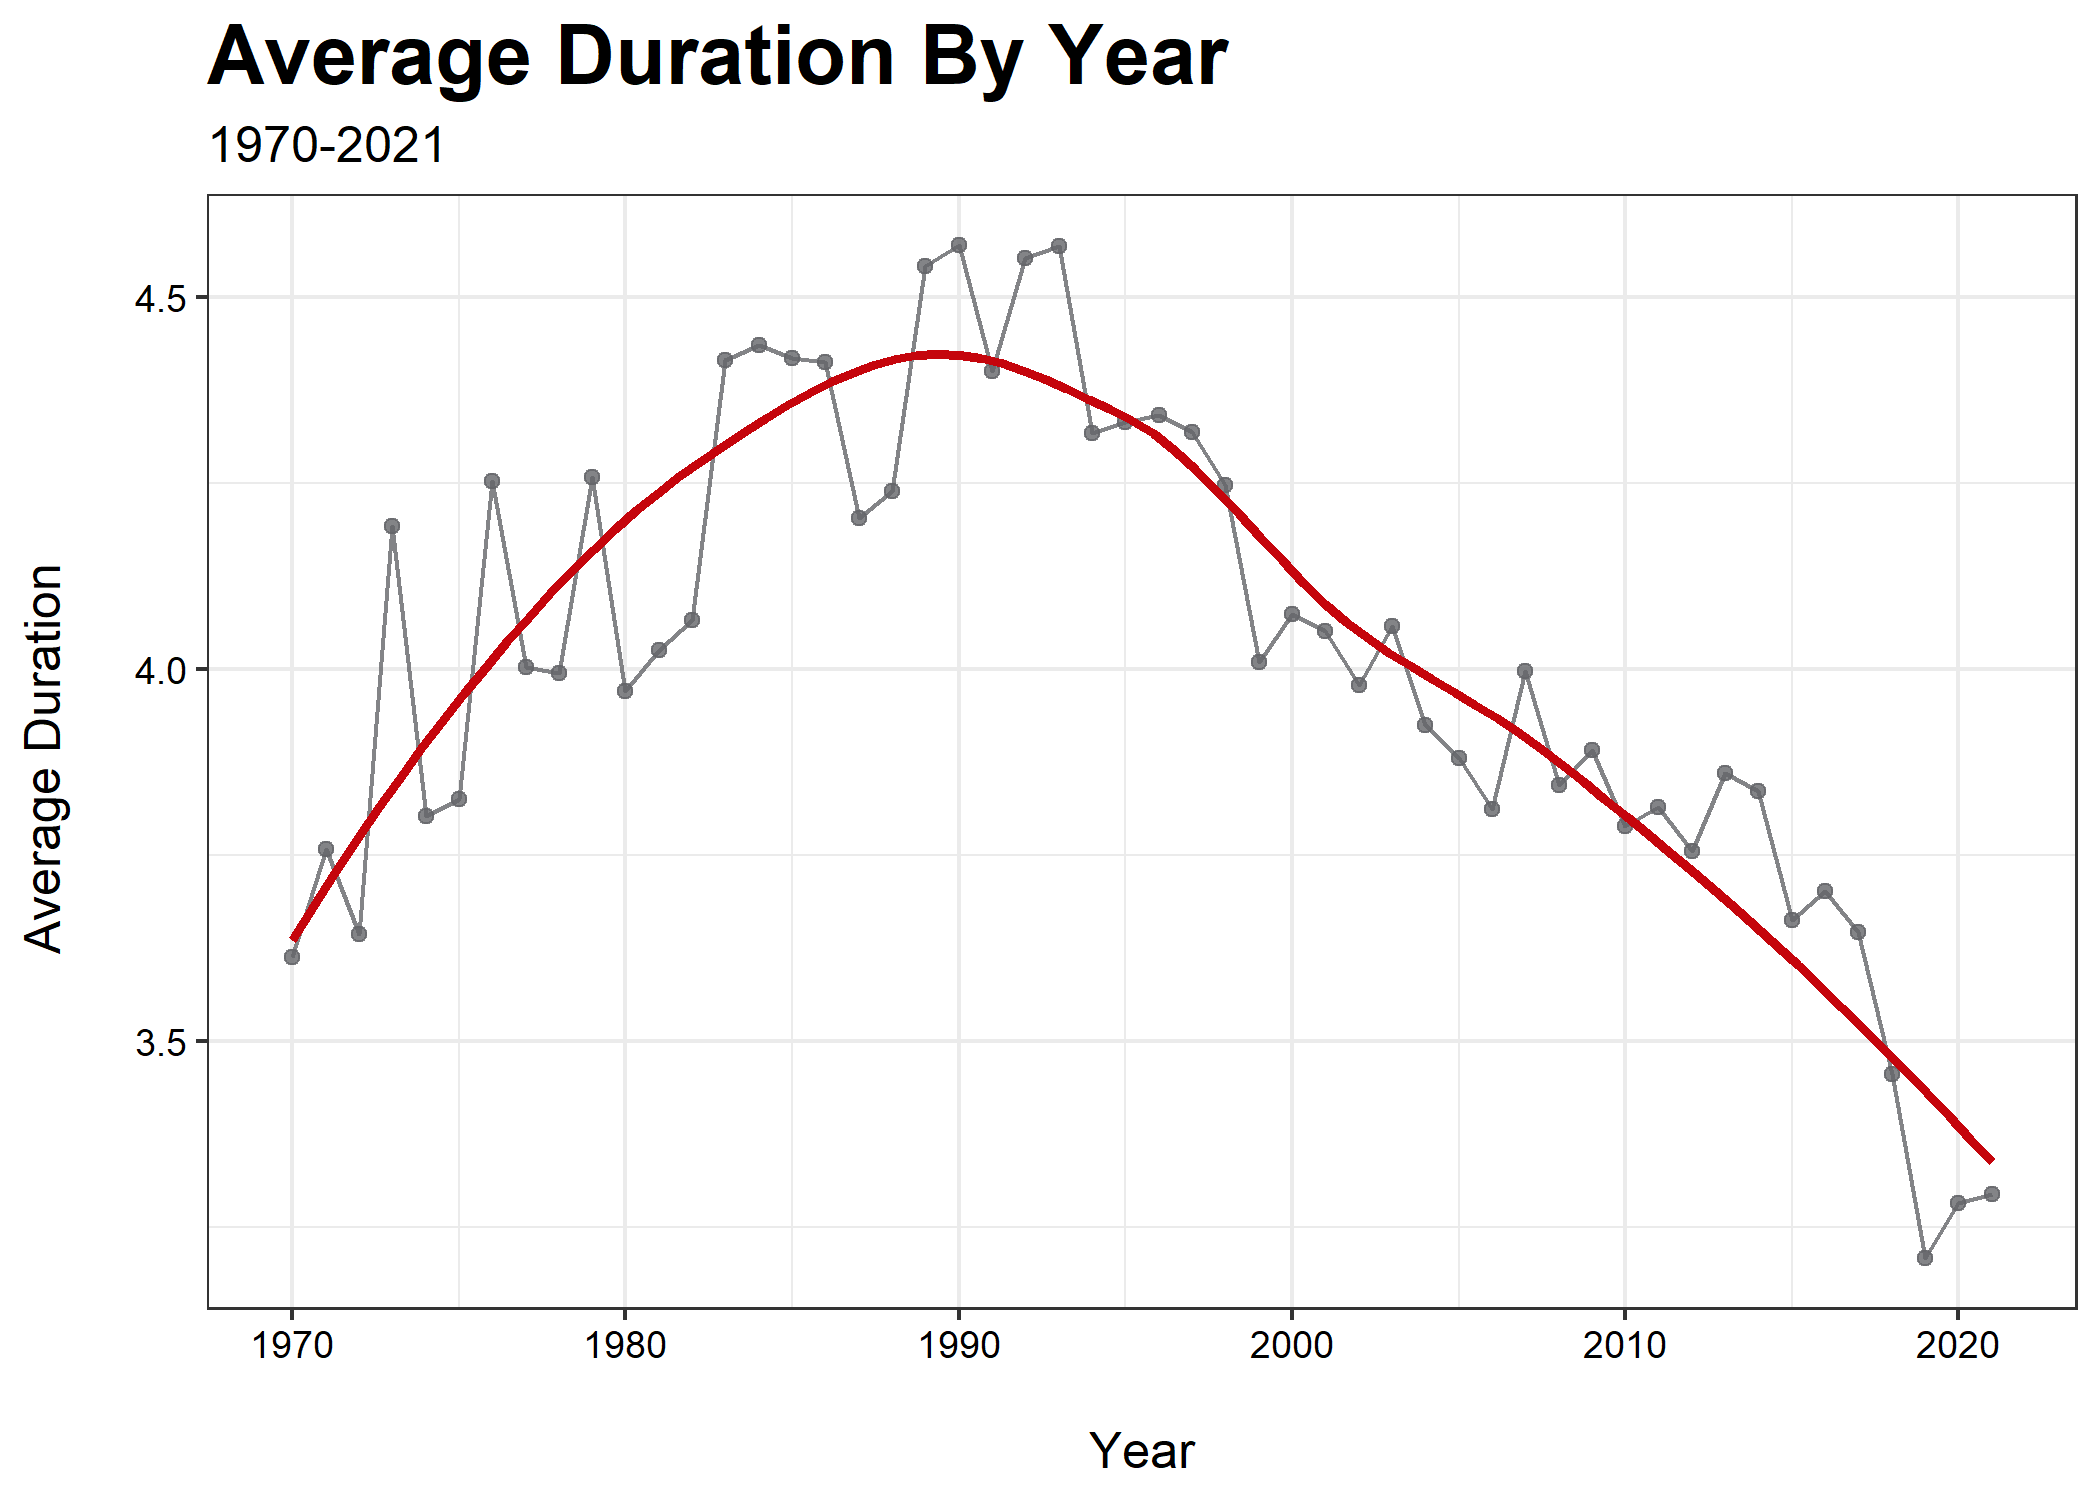
\includegraphics[width = \textwidth]{track_duration_trend_.png}
\caption{}
\label{fig:duration_trend}
\end{subfigure}
\caption{Trends in danceability, instrumnetalness, loudness, and duration metrics by year. Popular songs were, on average, getting louder and louder from about 1990 up until around 2010. We also observe a sharp decline in average instrumentalness around 1995. These figures also highlight the importance of considering temporal correlation within the data---songs within particularly periods of time are, on average, similar in their audio features.}
\label{fig:multipart_figure}
\end{figure}
% Further, it's not surprising that there is some apparent colinearity among the predictors. Intuitively, we'd expect songs high in acousticness to also score low in loudness, for example.

% \begin{figure}[H] % H forces the figure to appear in this location, h! tries really hard to do the same thing
% \centering
% 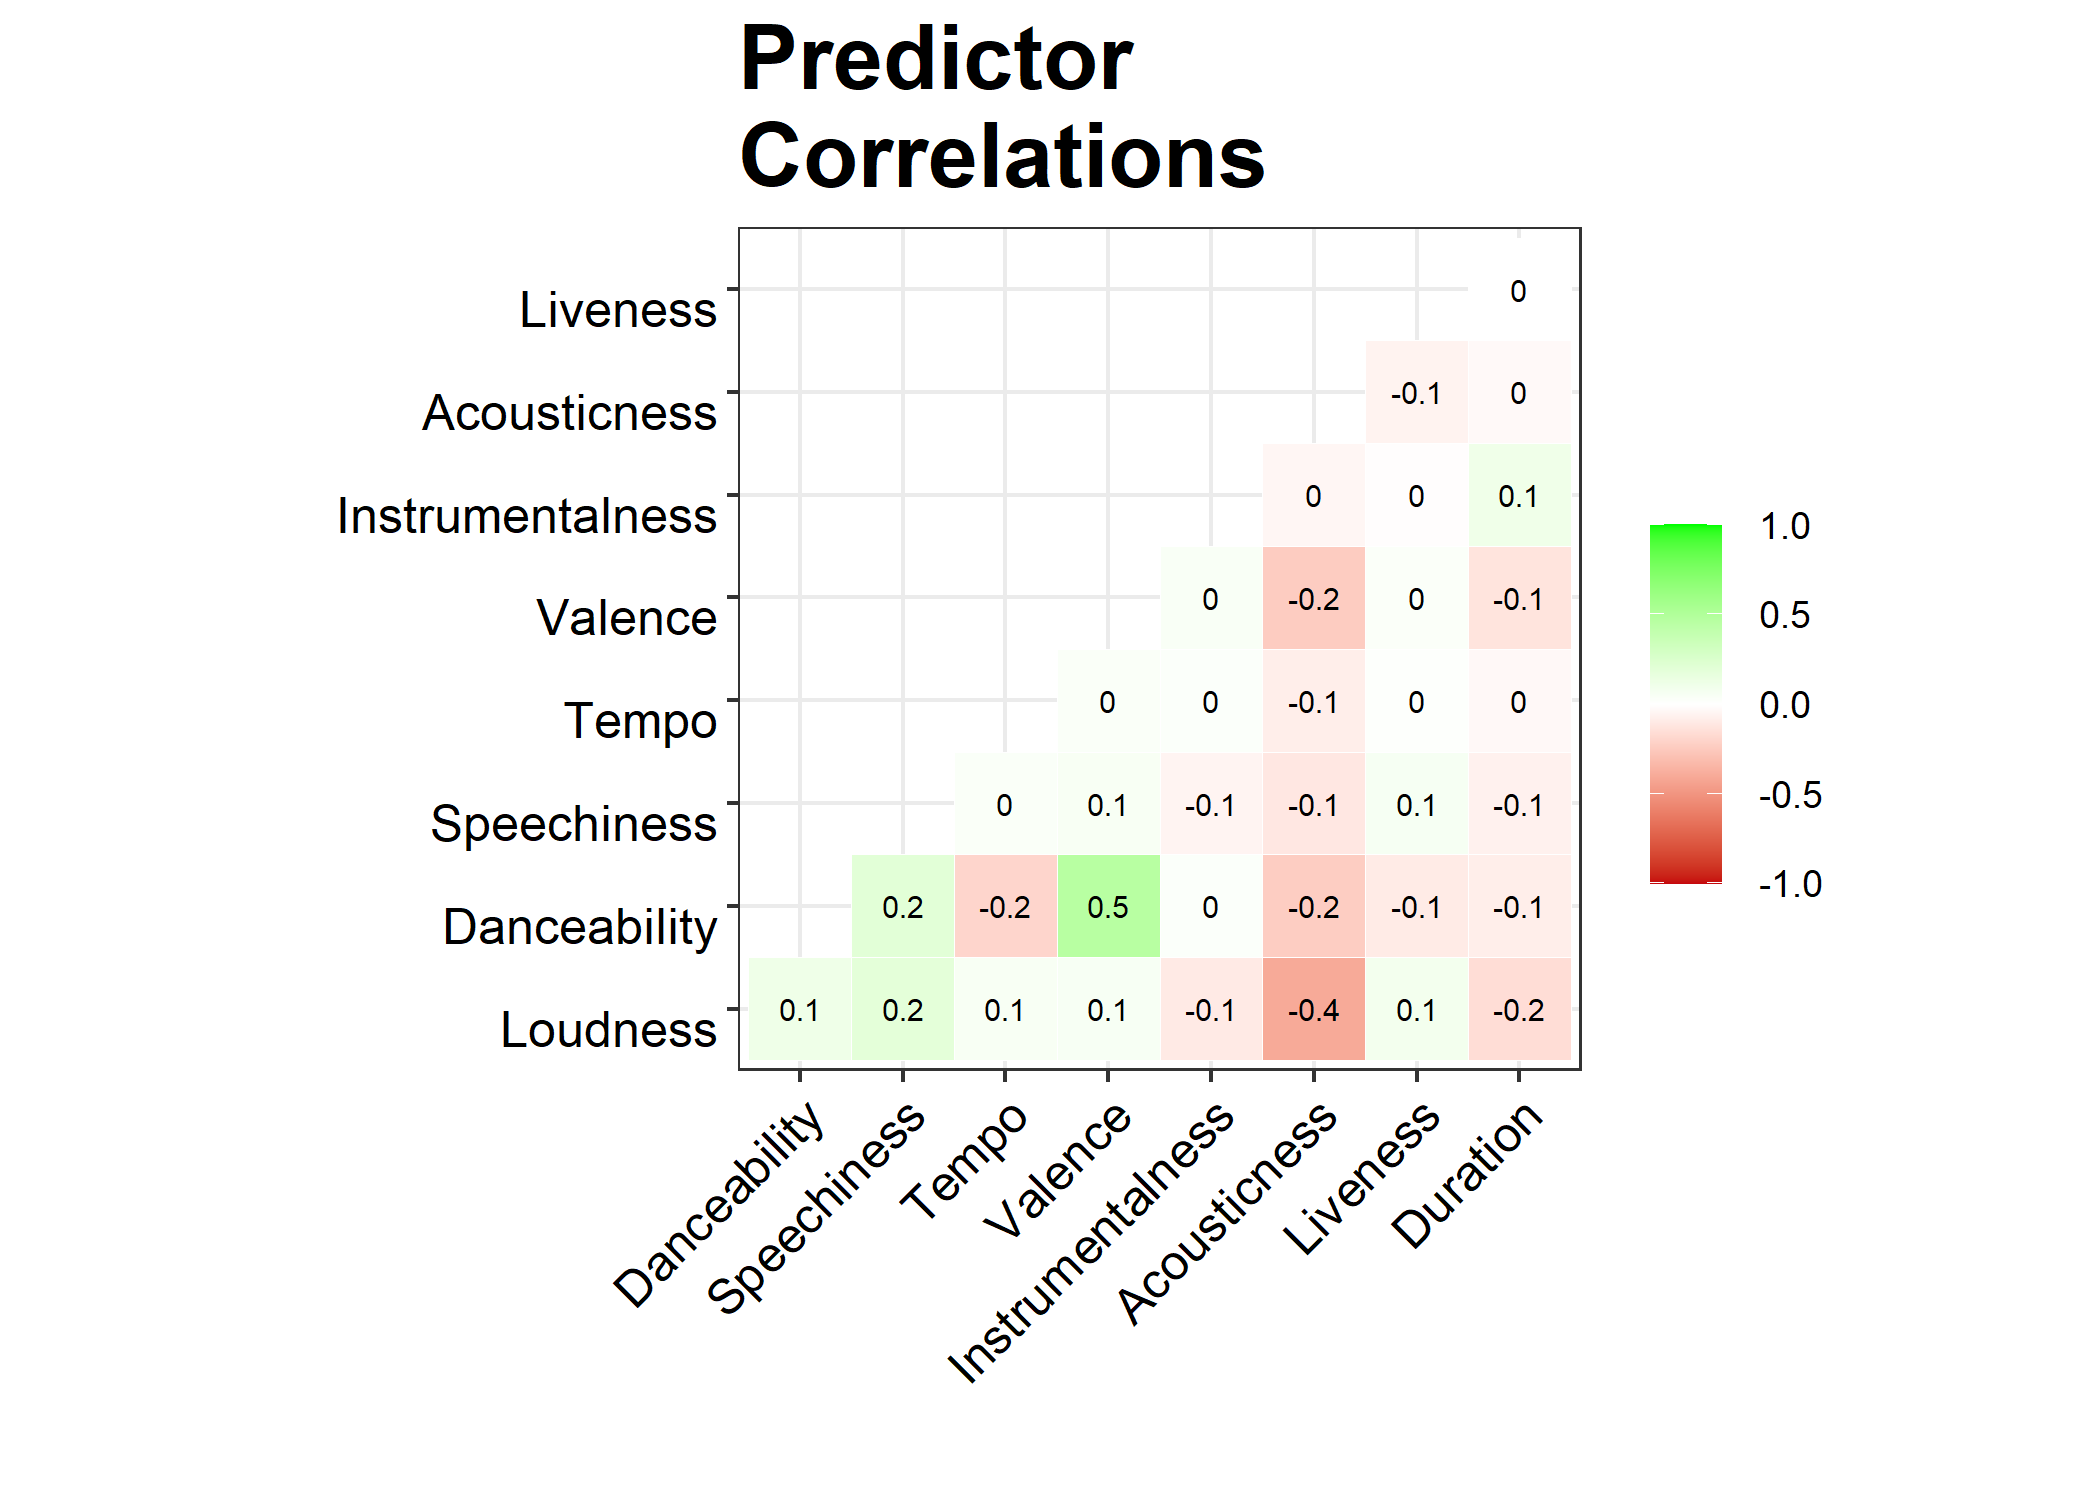
\includegraphics[width=1\textwidth]{predictor_correlations.png} % no need to specify a file extension & pay attention to scaling by width!
% \caption{}
% \label{fig:predictor_cor} % useful for hyperref'ing later
% \end{figure}
The primary interest is in the relationship between the predictors and popularity. I consider 10 predictors. Visual inspection suggests, surprisingly, that these relationships are weak:

\begin{figure}[H]
\begin{subfigure}[b]{0.5\textwidth}
\centering
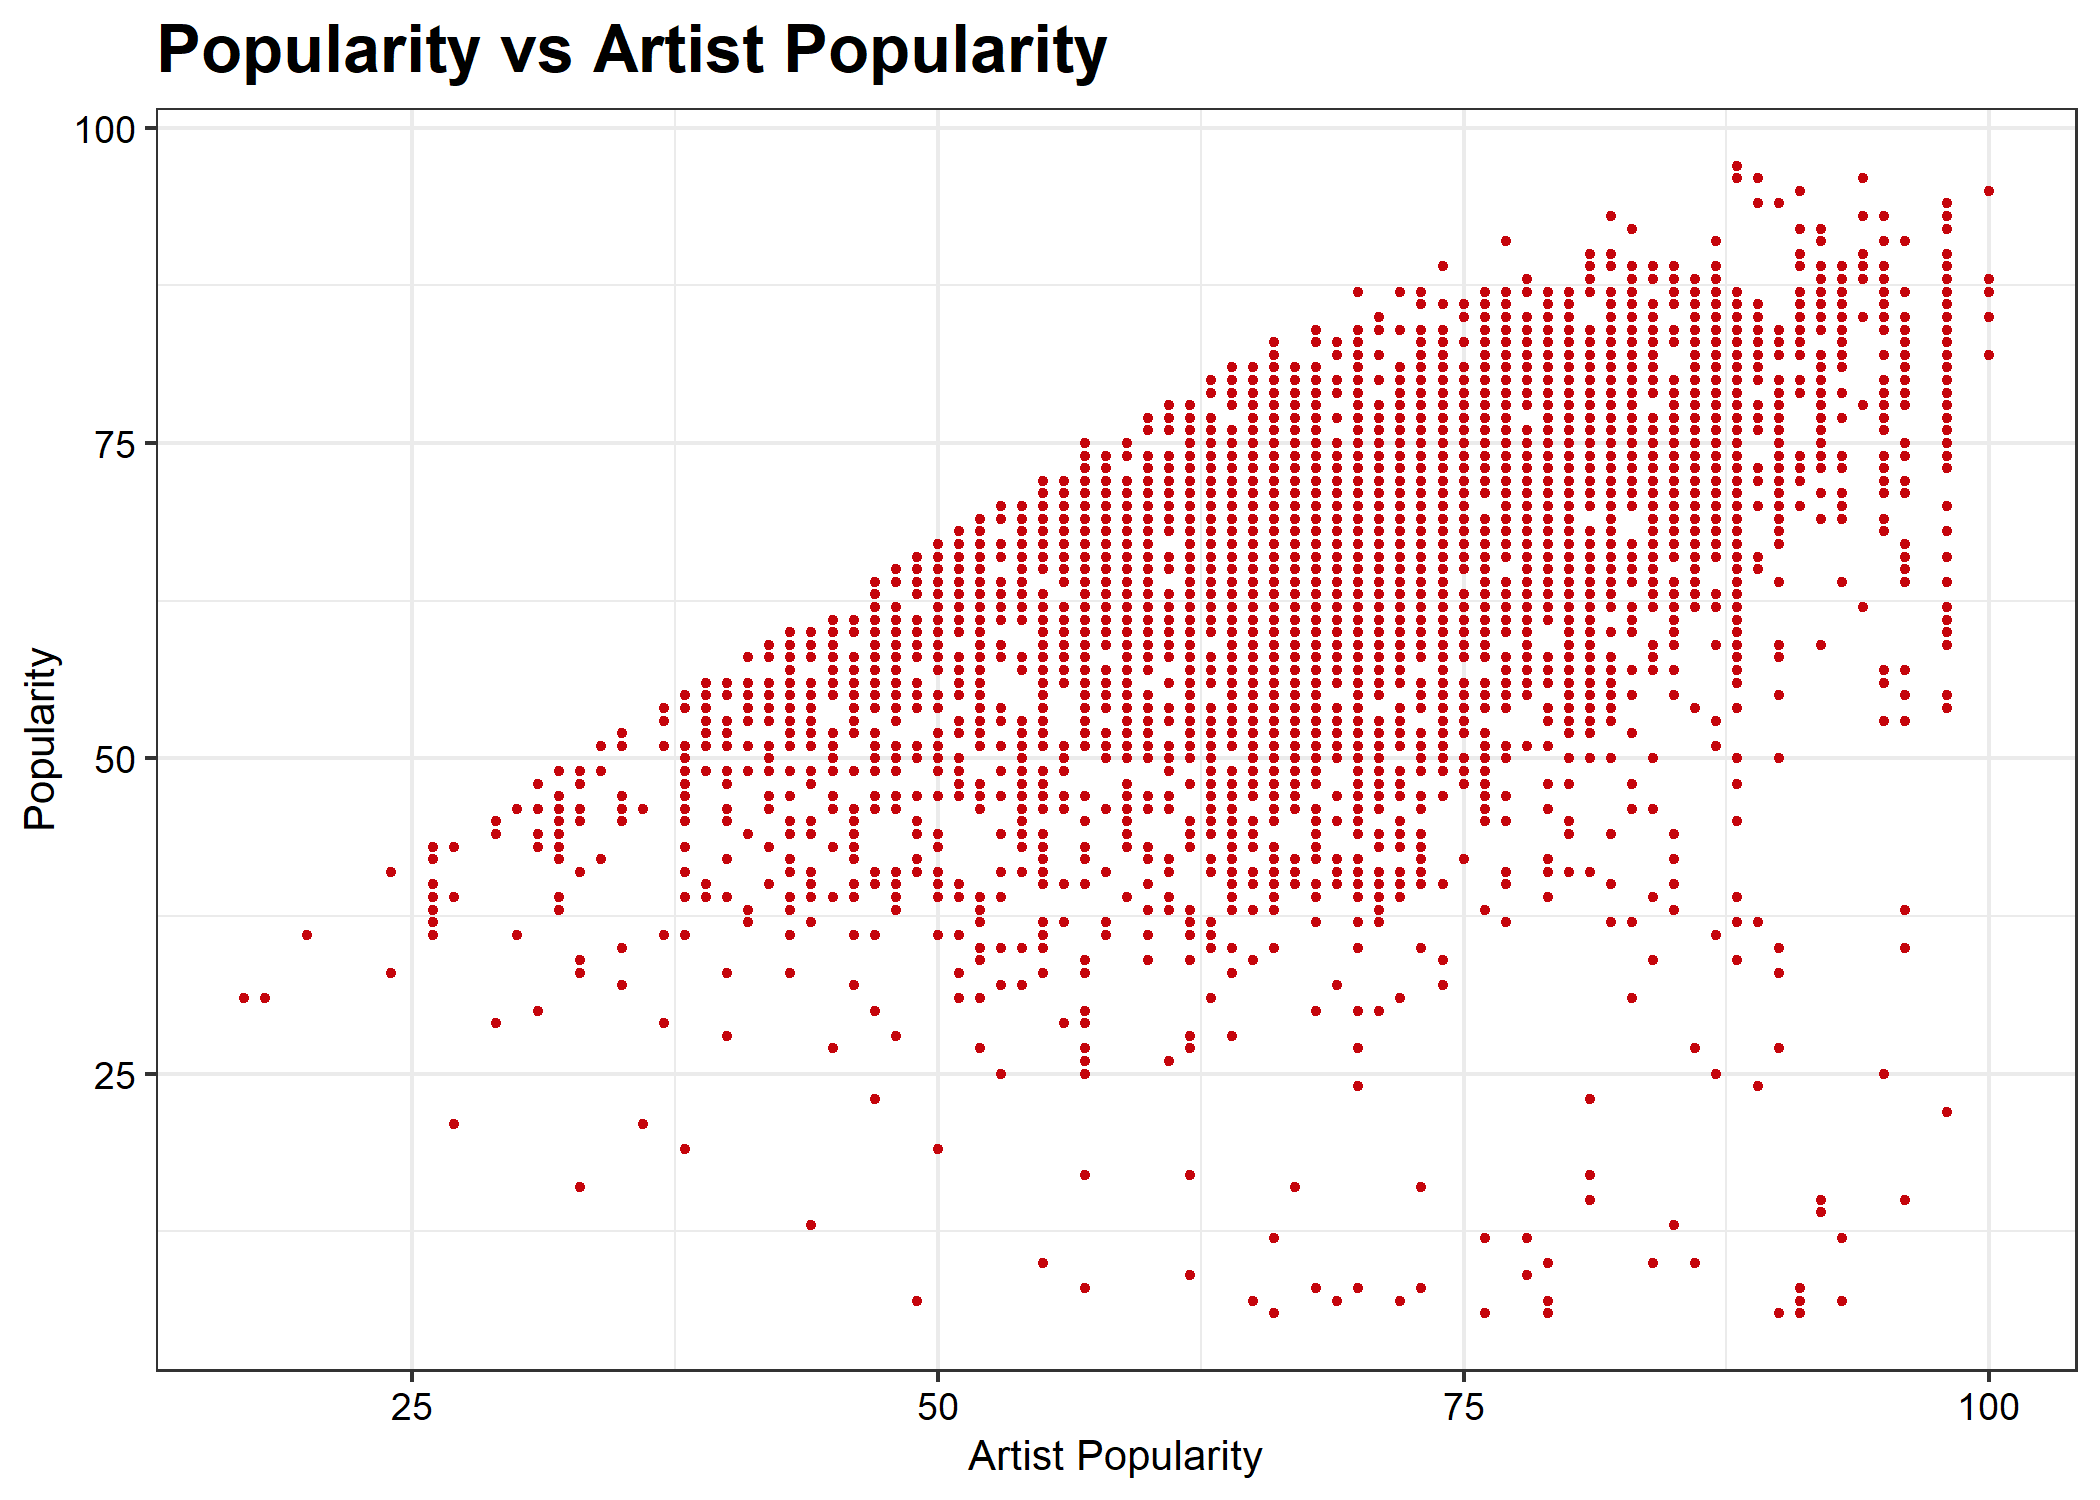
\includegraphics[width = \textwidth]{pop_vs_artist_pop.png}
\caption{}
\label{fig:danceability_trend}
\end{subfigure}
\begin{subfigure}[b]{0.5\textwidth}
\centering
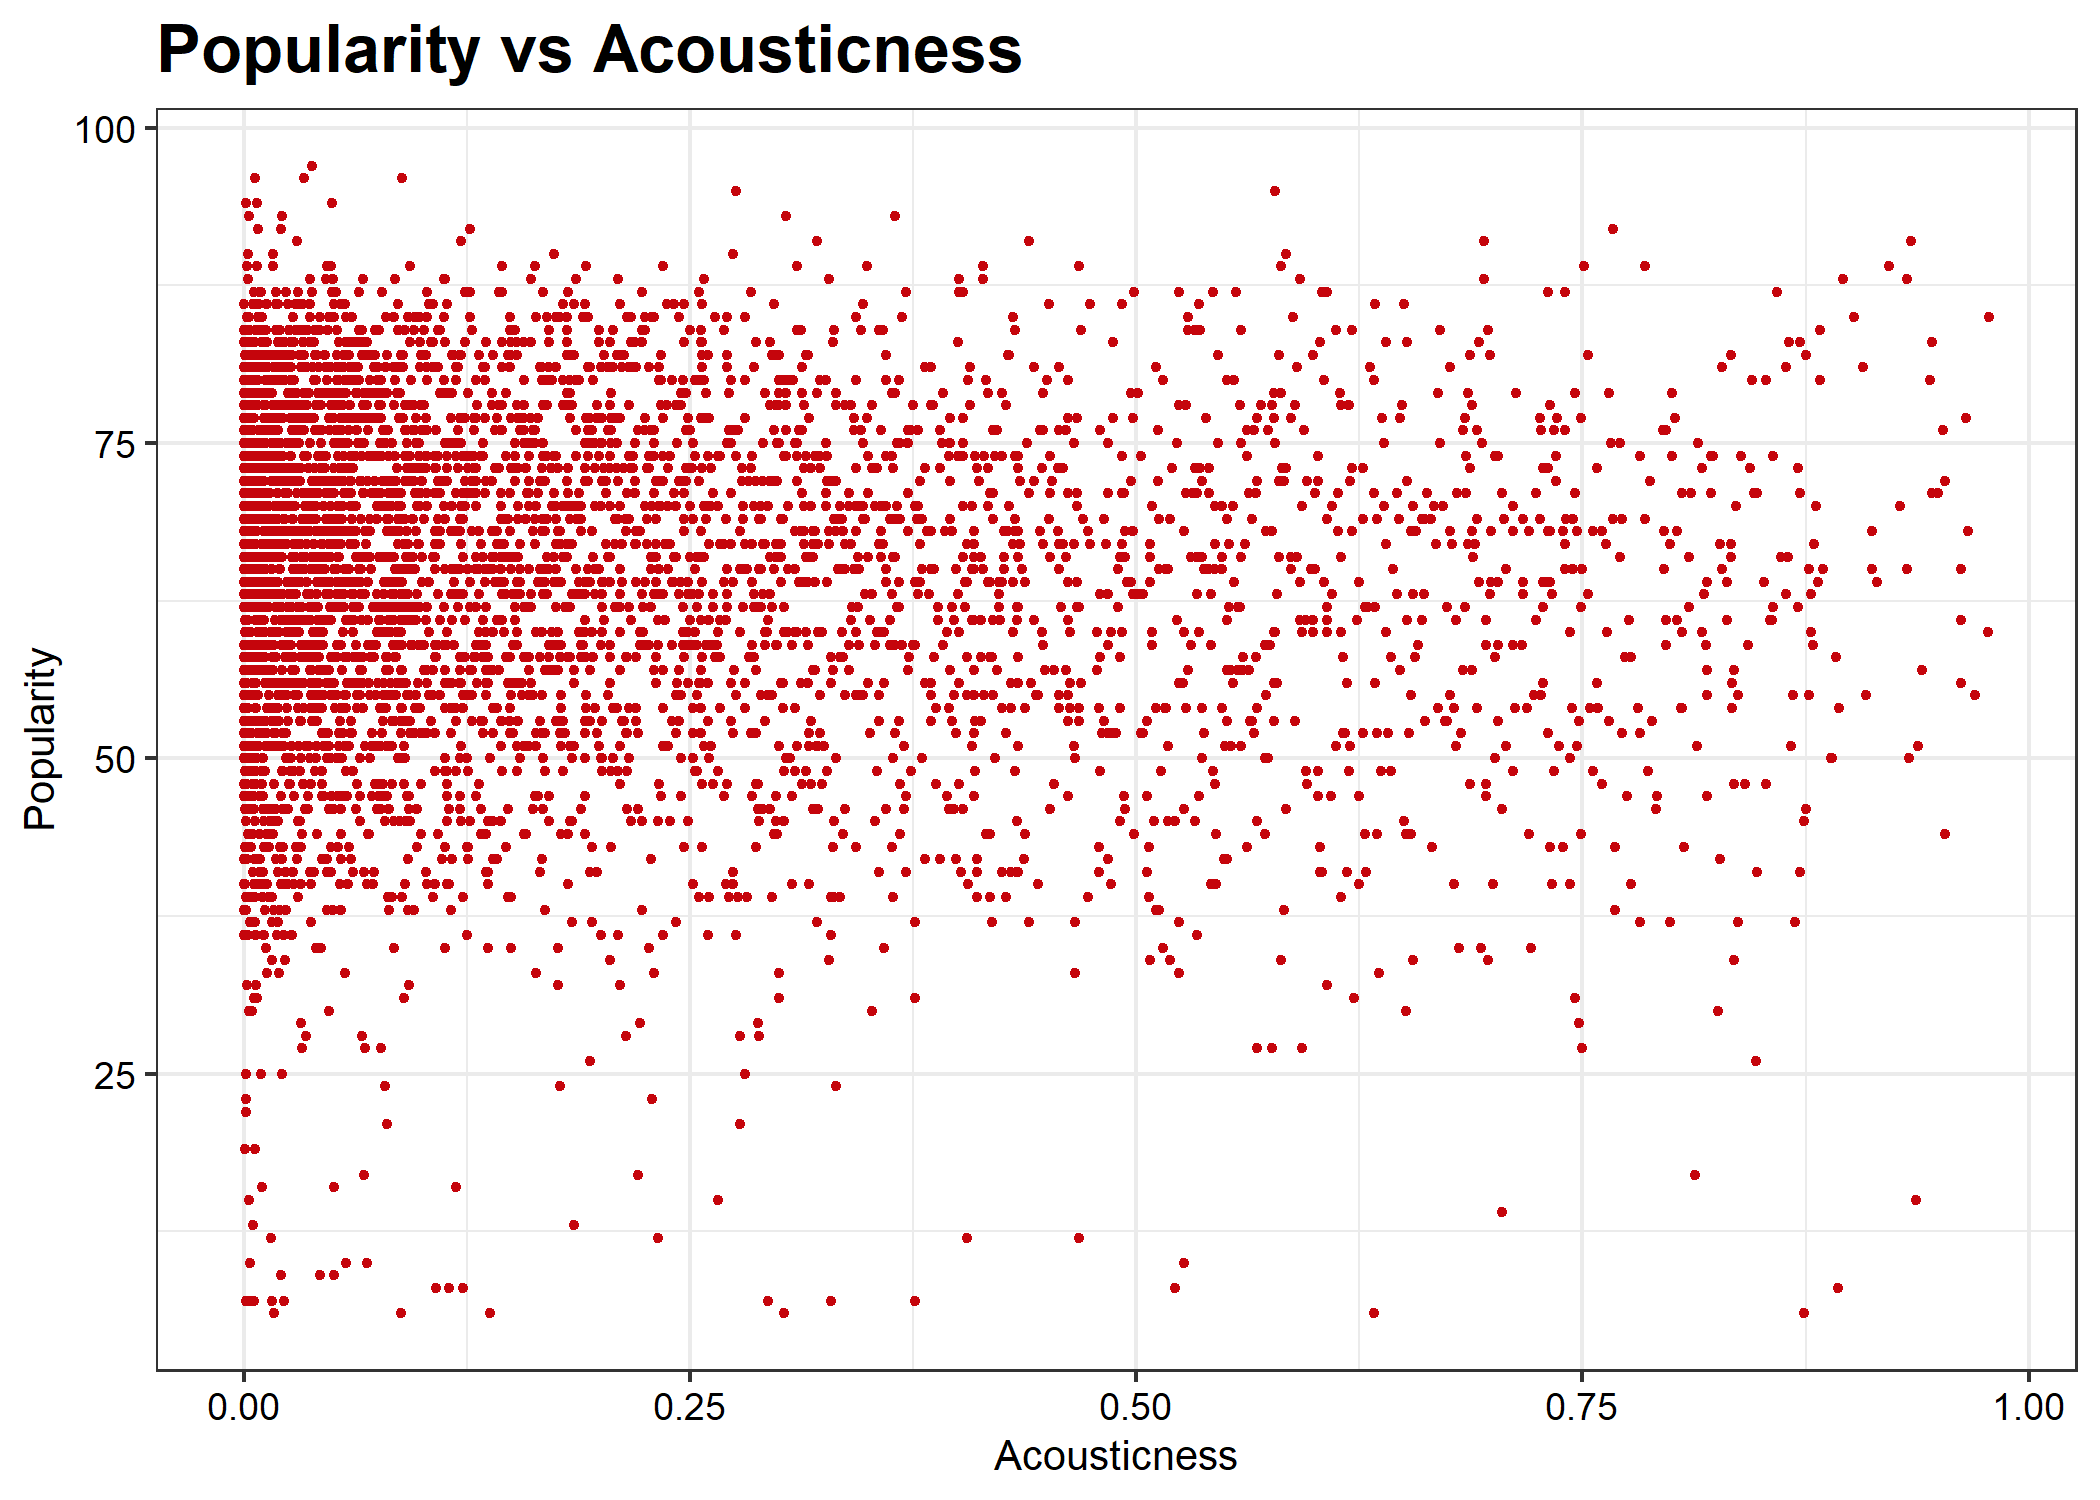
\includegraphics[width = \textwidth]{pop_vs_track_acousticness.png}
\caption{}
\label{fig:instrumentalness_trend}
\end{subfigure}
\begin{subfigure}[b]{0.5\textwidth}
\centering
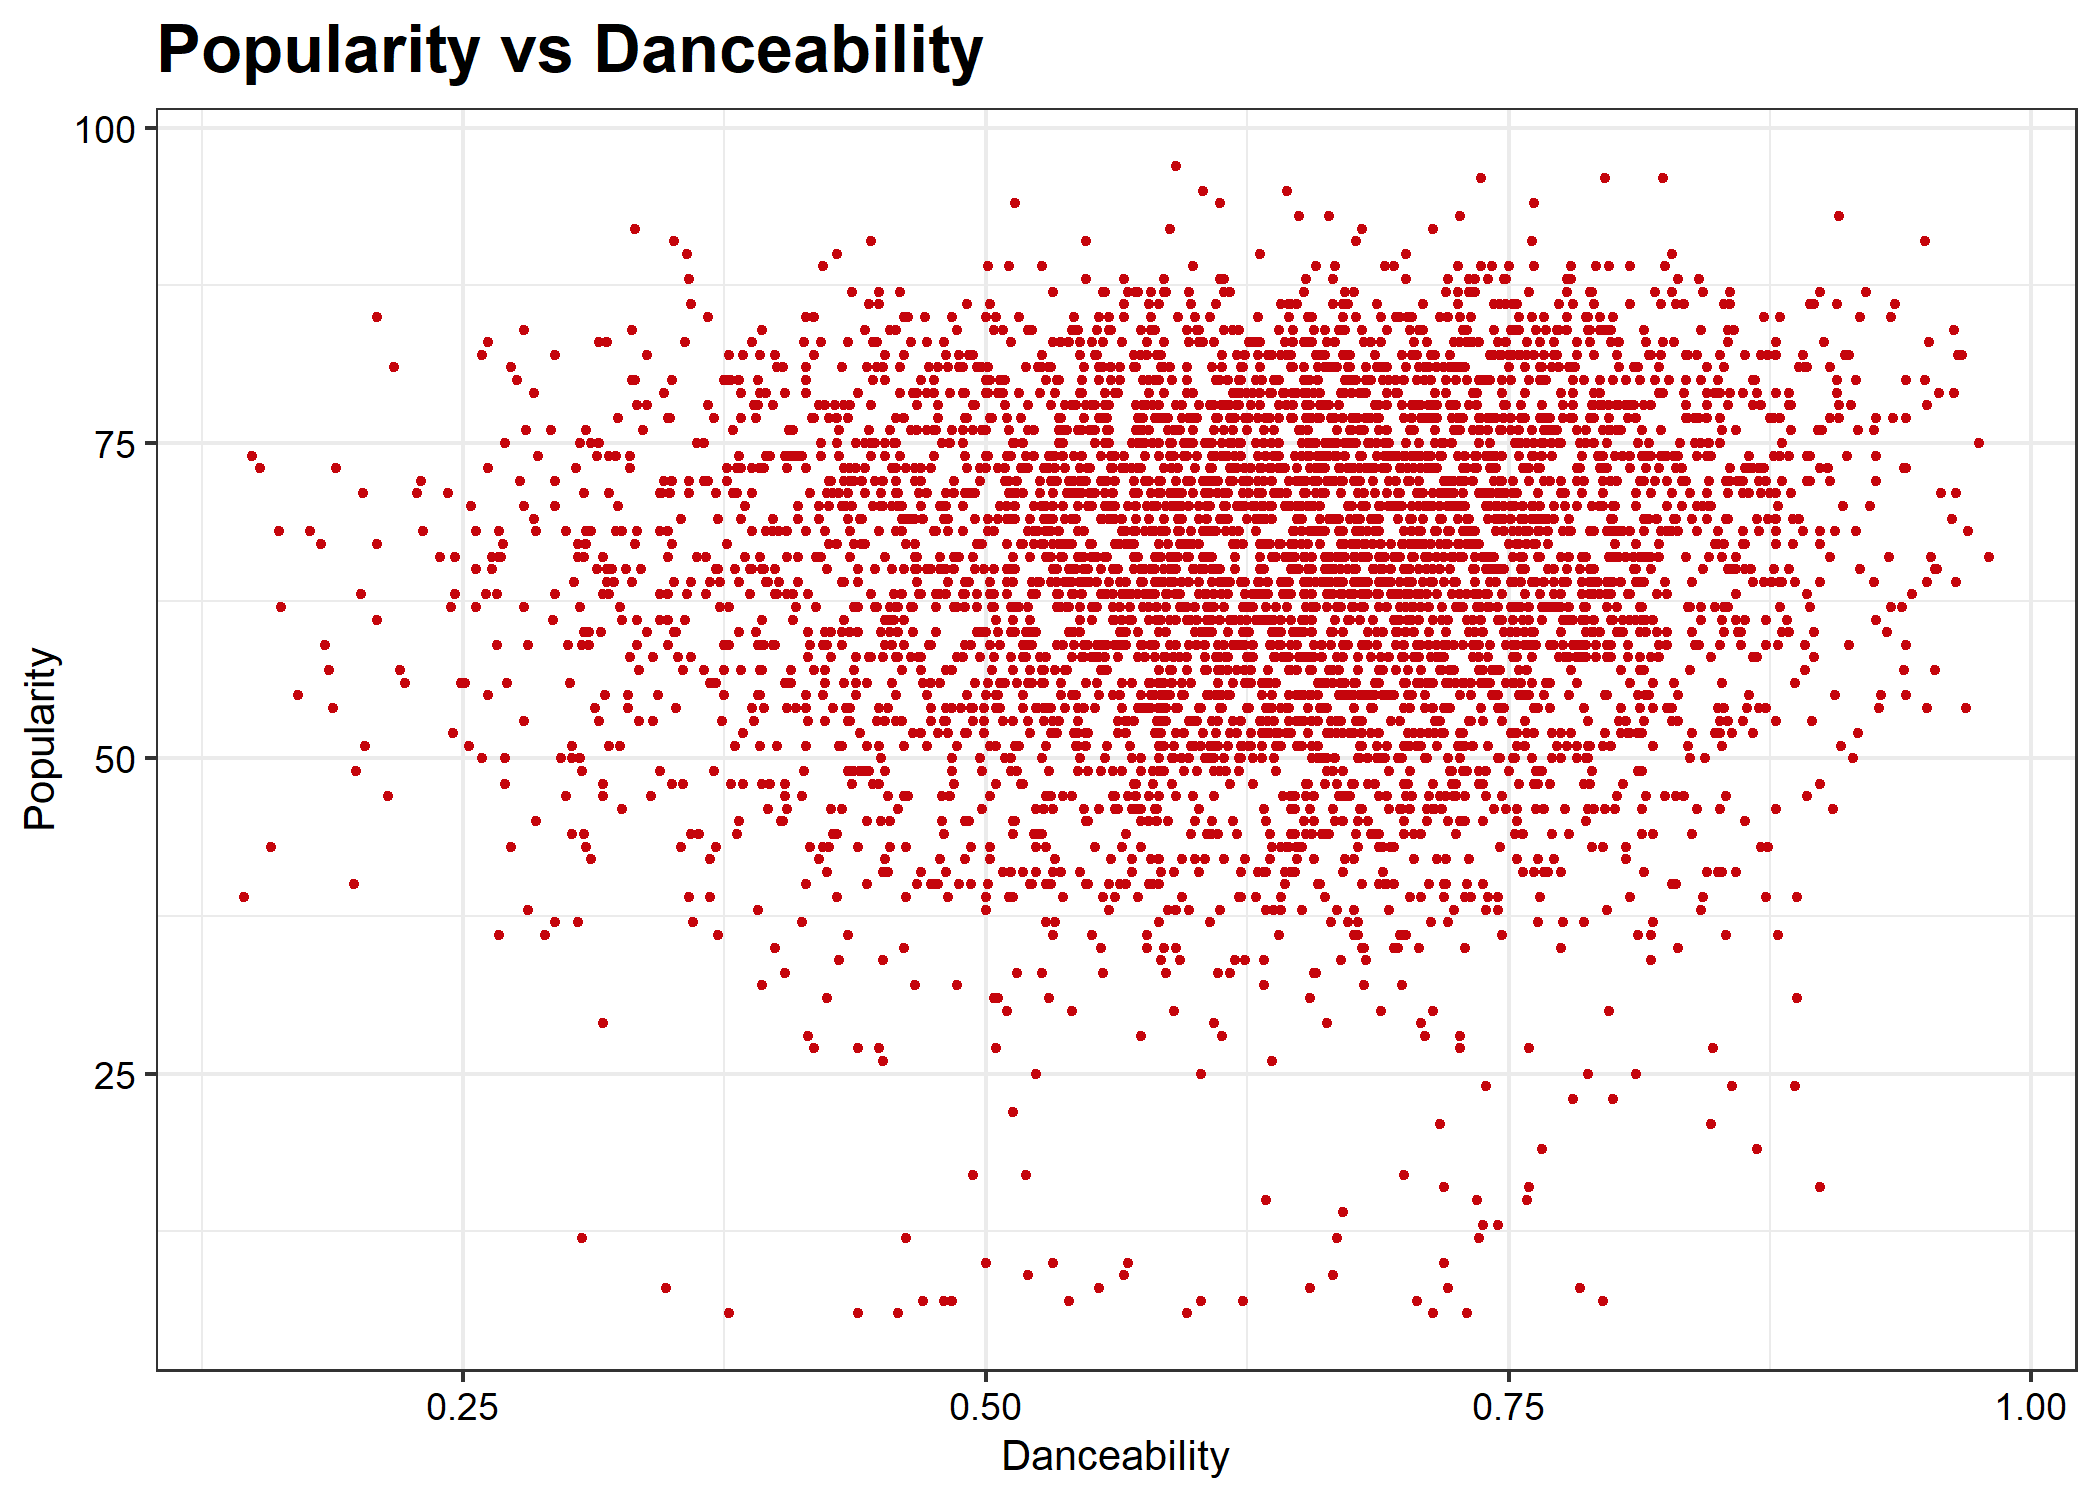
\includegraphics[width = \textwidth]{pop_vs_track_danceability.png}
\caption{}
\label{fig:loudness_trend}
\end{subfigure}
\begin{subfigure}[b]{0.5\textwidth}
\centering
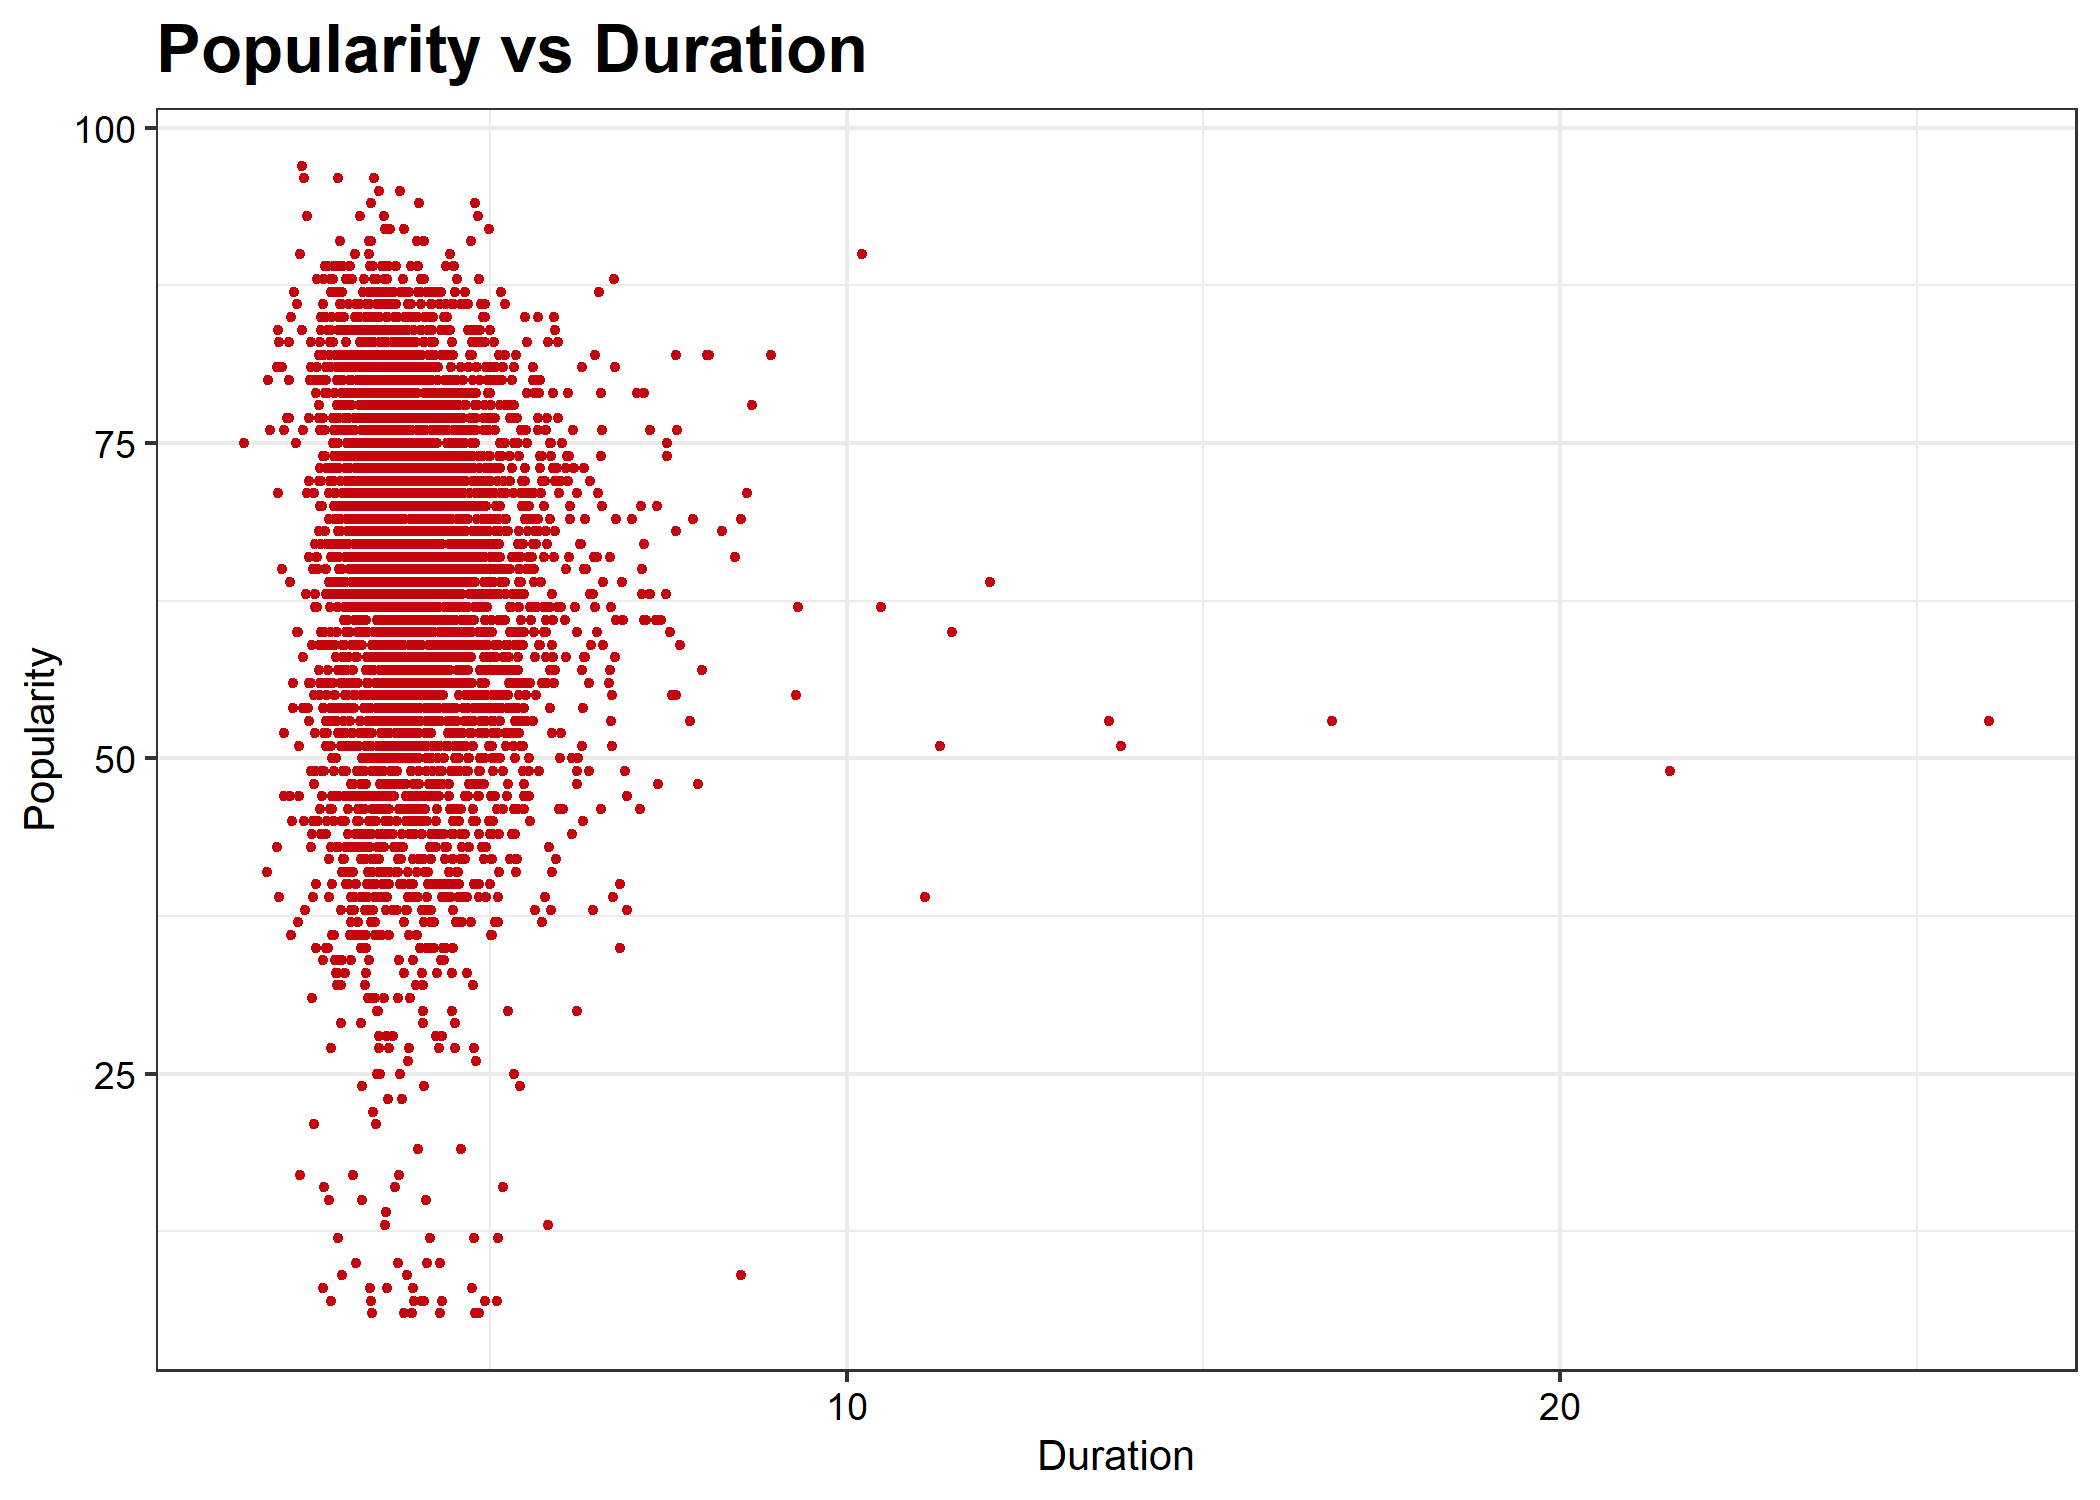
\includegraphics[width = \textwidth]{pop_vs_track_duration.png}
\caption{}
\label{fig:duration_trend}
\end{subfigure}
\begin{subfigure}[b]{0.5\textwidth}
\centering
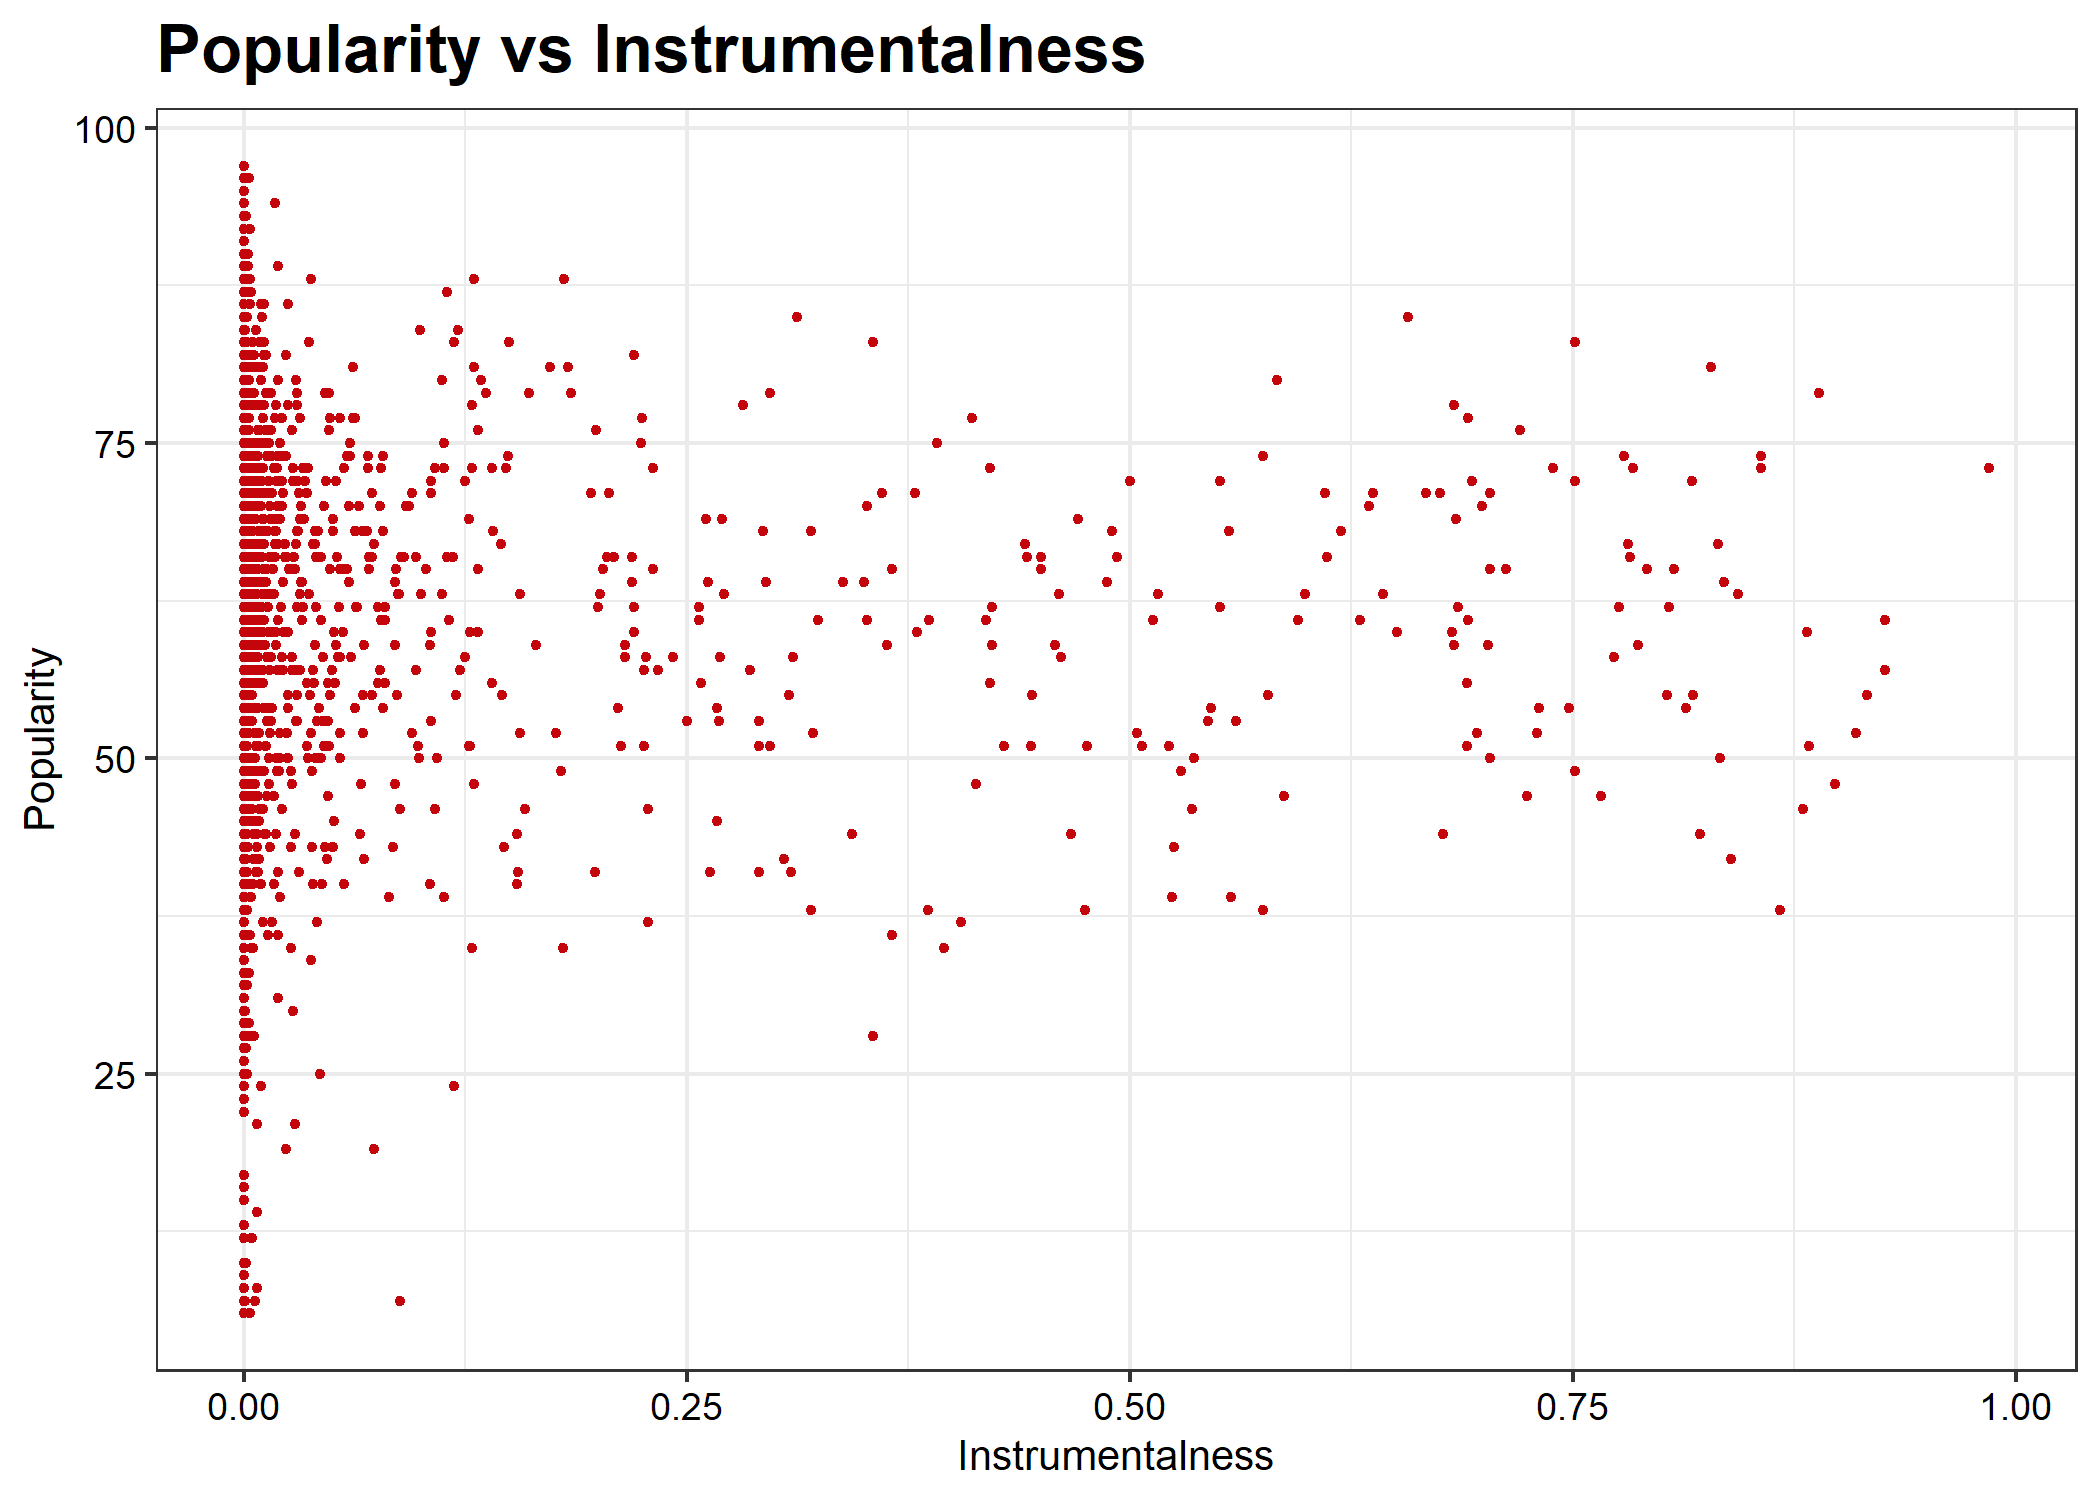
\includegraphics[width = \textwidth]{pop_vs_track_instrumentalness.png}
\caption{}
\label{fig:duration_trend}
\end{subfigure}
\begin{subfigure}[b]{0.5\textwidth}
\centering
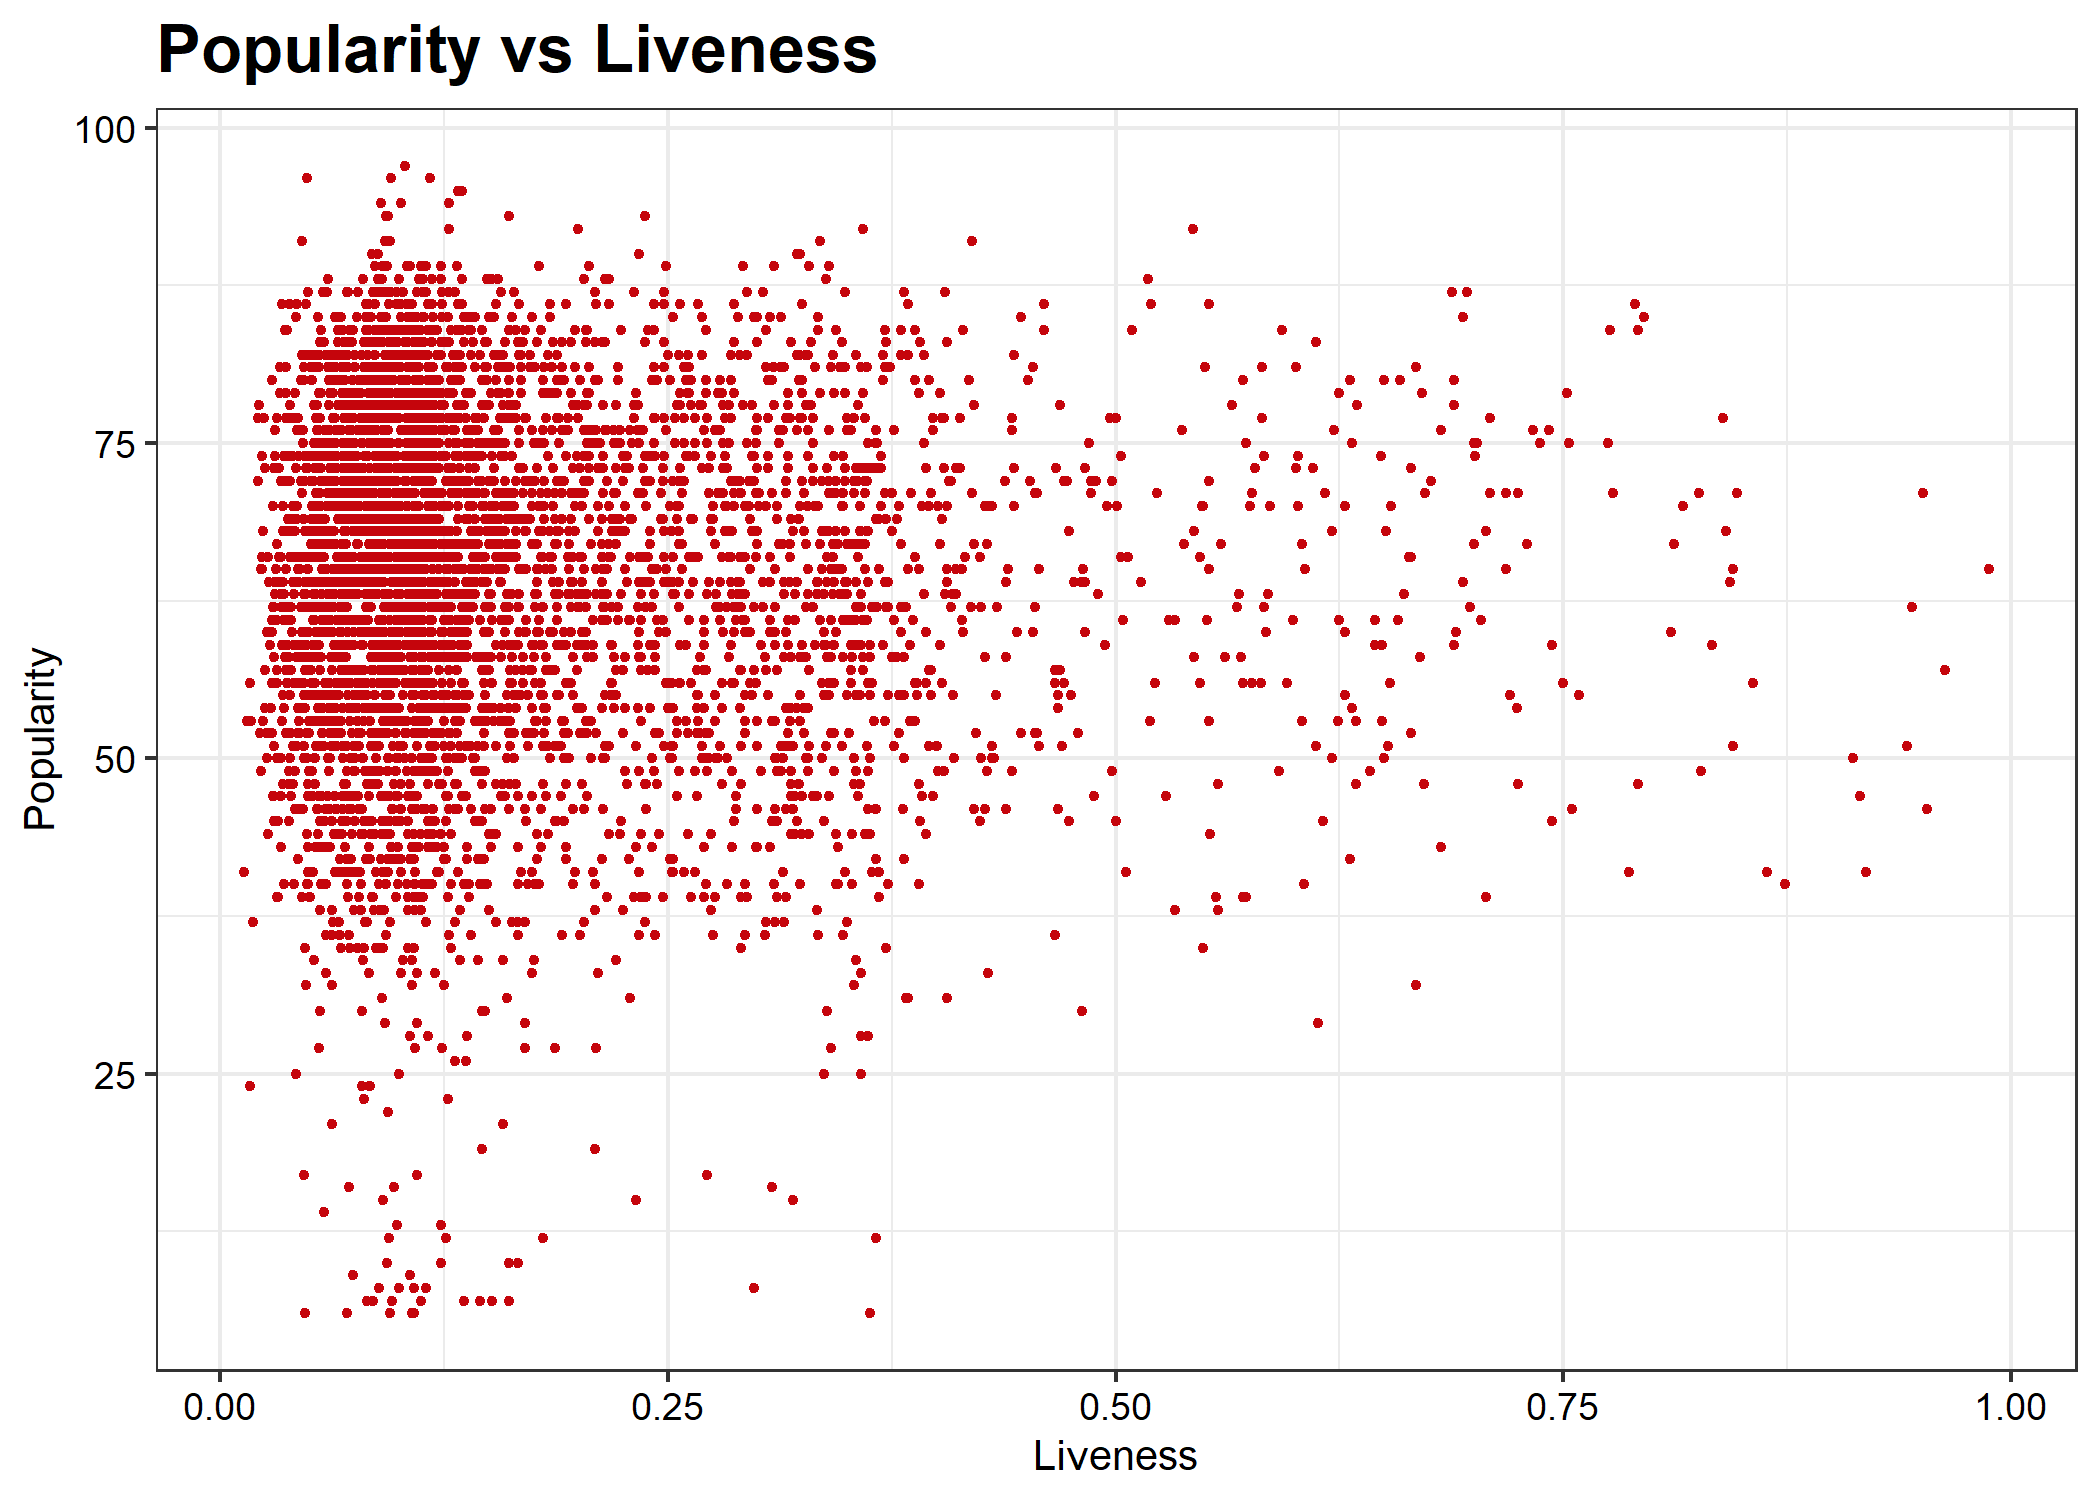
\includegraphics[width = \textwidth]{pop_vs_track_liveness.png}
\caption{}
\label{fig:duration_trend}
\end{subfigure}
\label{fig:multipart_figure}
\end{figure}

\begin{figure}[H]
\ContinuedFloat
\begin{subfigure}[b]{0.5\textwidth}
\centering
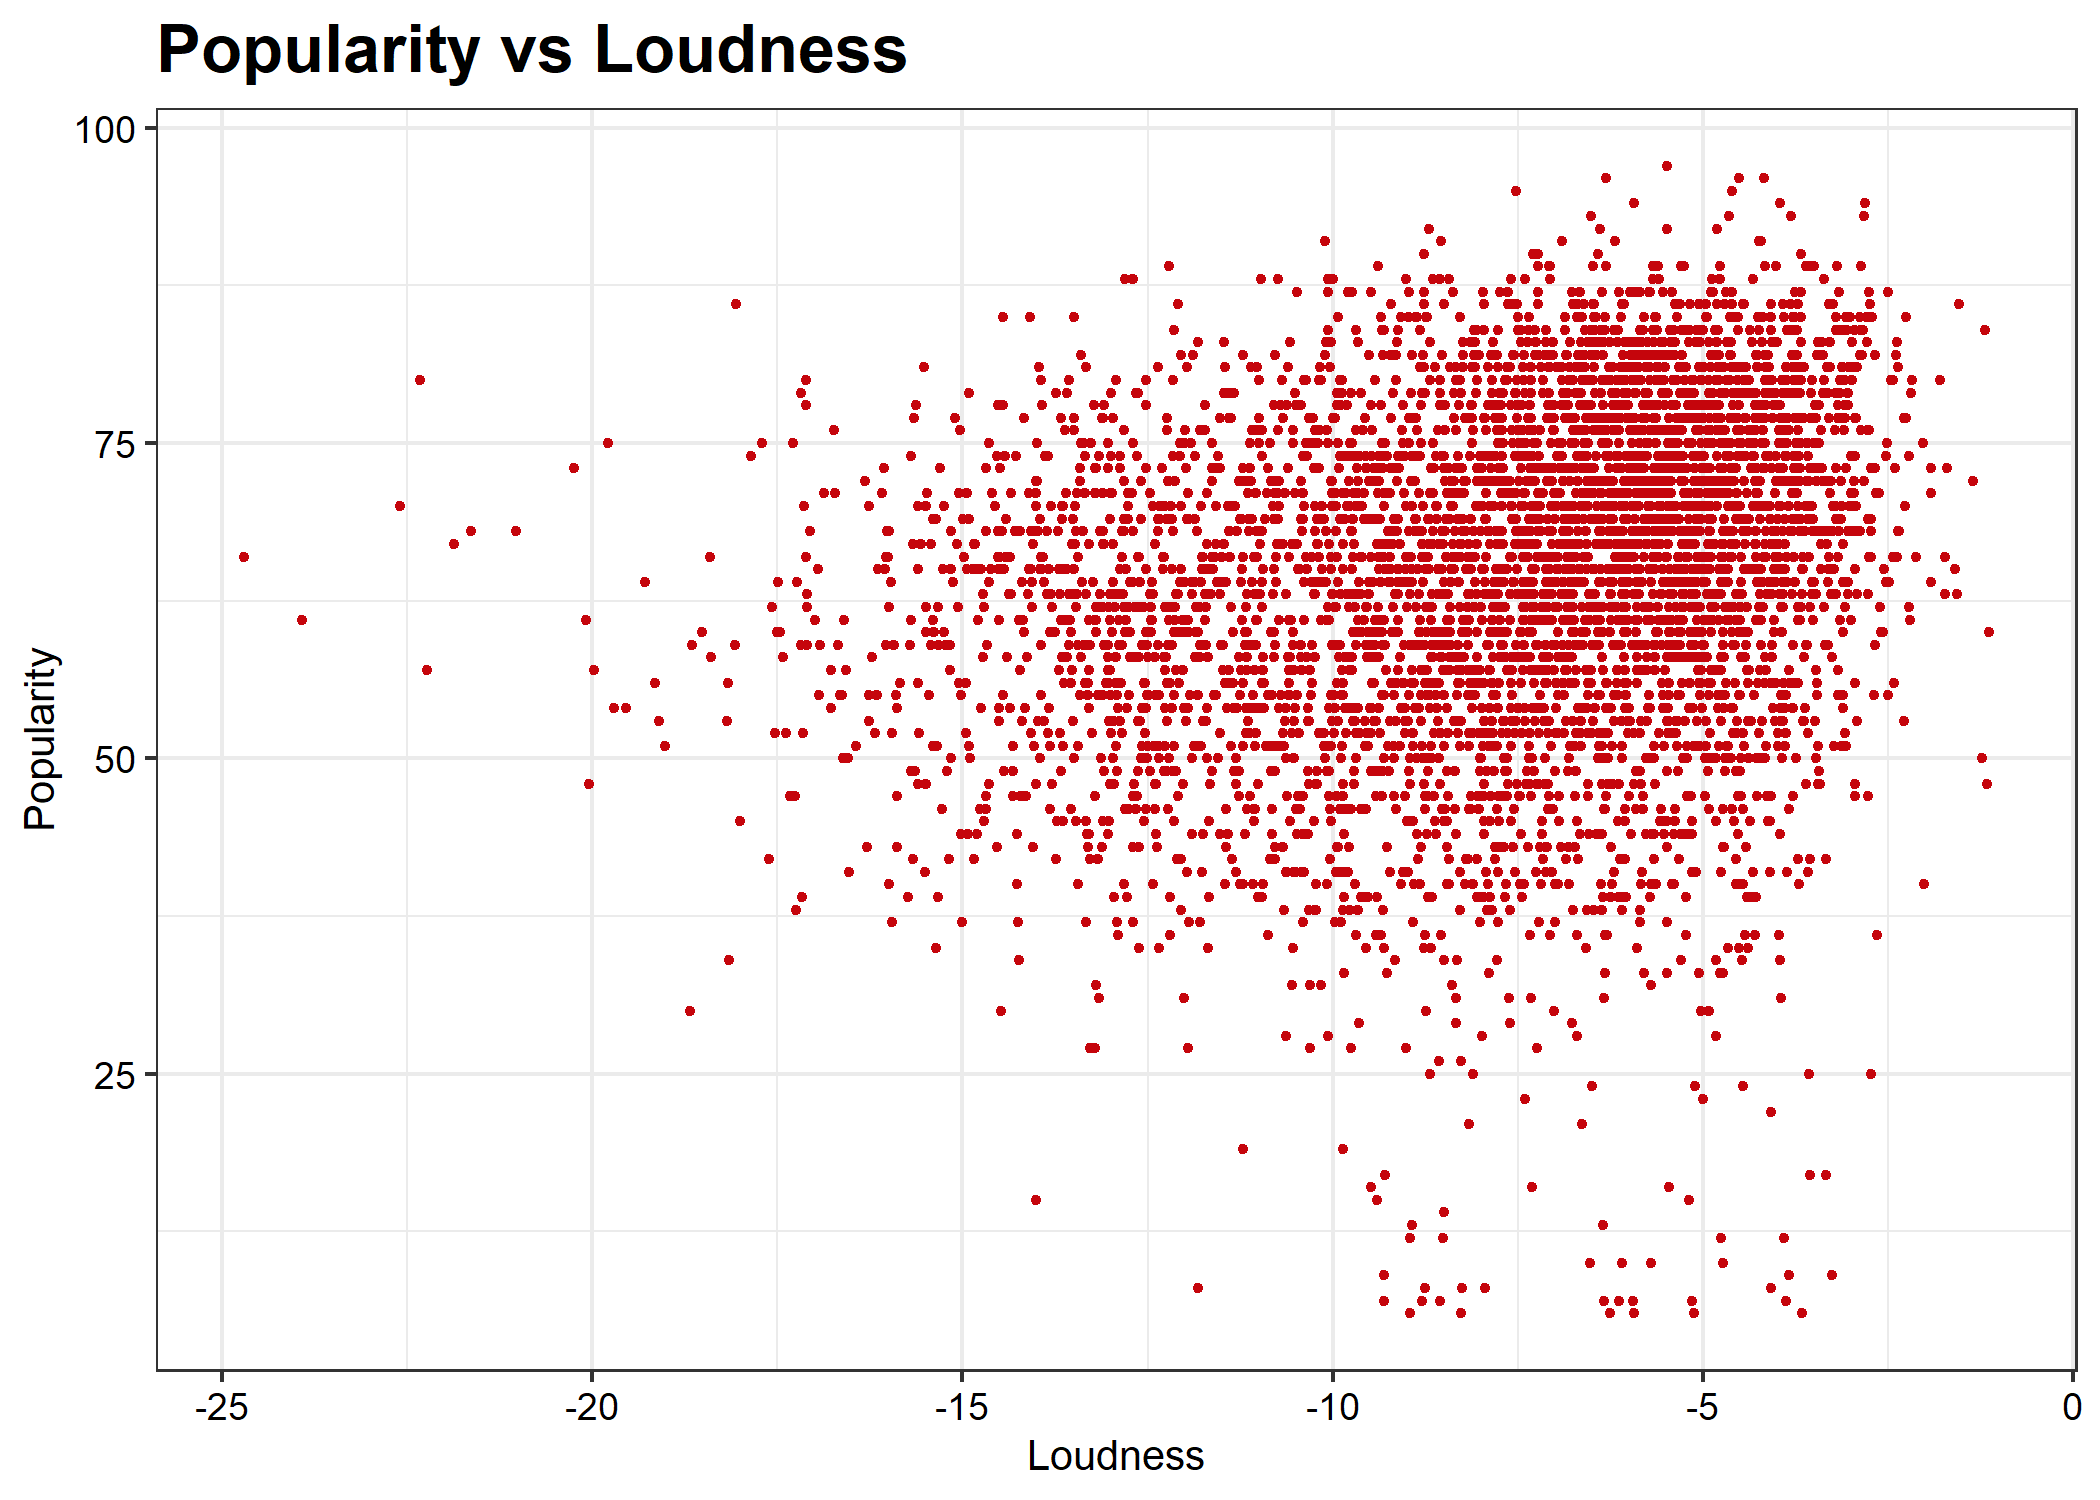
\includegraphics[width = \textwidth]{pop_vs_track_loudness.png}
\caption{}
\label{fig:duration_trend}
\end{subfigure}
\begin{subfigure}[b]{0.5\textwidth}
\centering
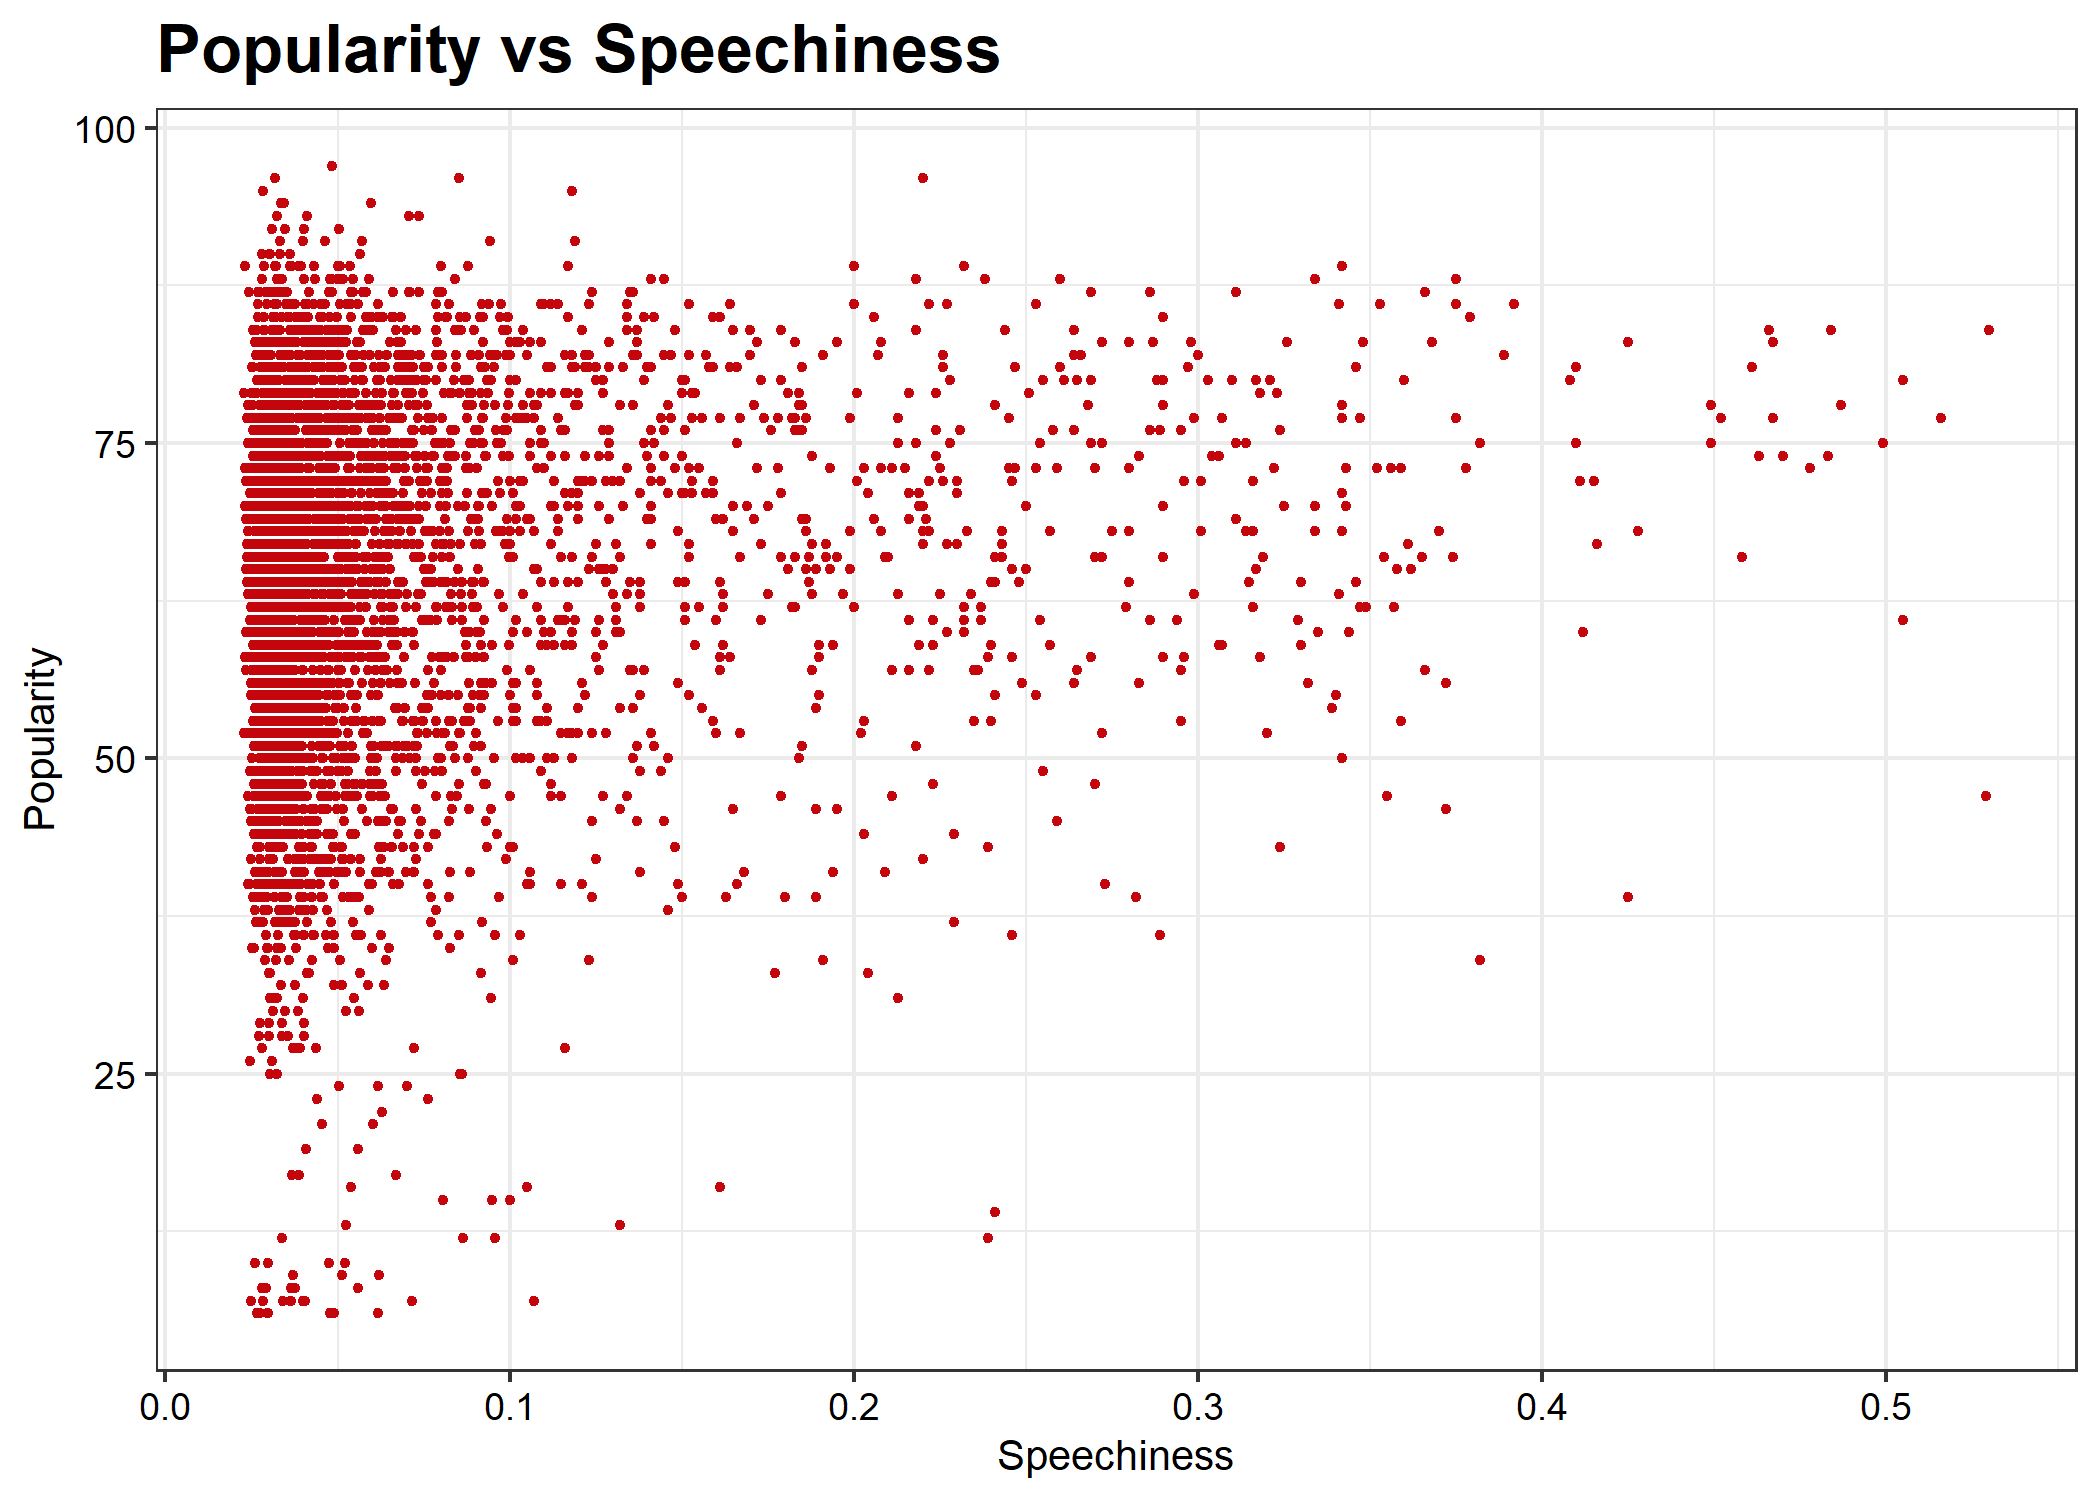
\includegraphics[width = \textwidth]{pop_vs_track_speechiness.png}
\caption{}
\label{fig:duration_trend}
\end{subfigure}
\begin{subfigure}[b]{0.5\textwidth}
\centering
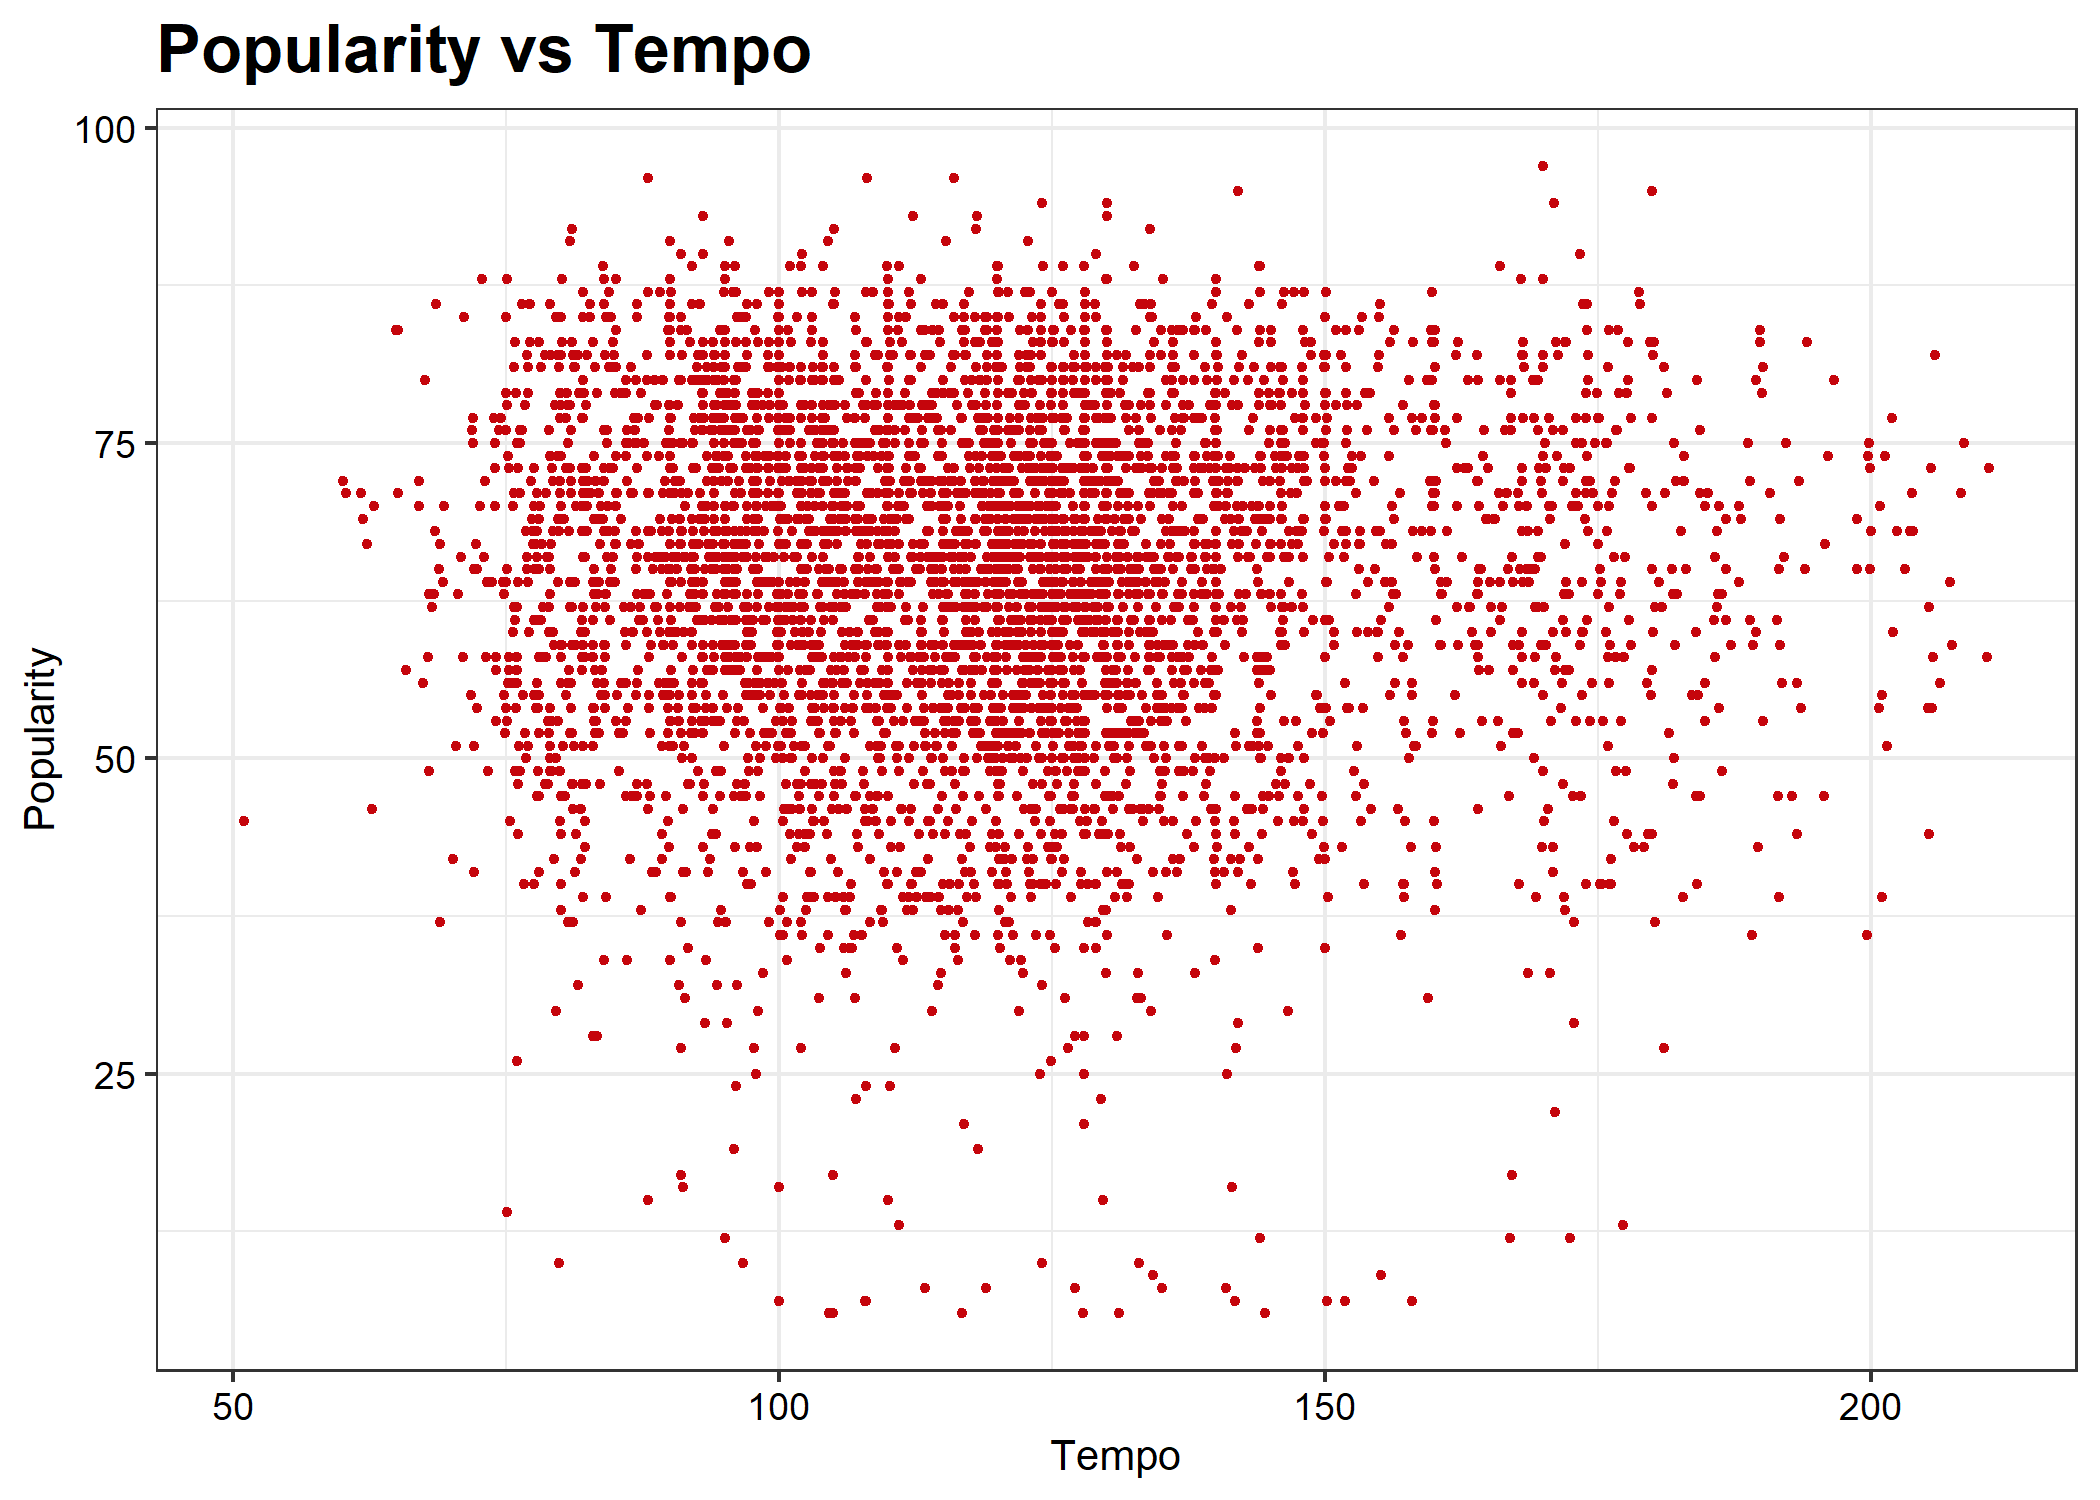
\includegraphics[width = \textwidth]{pop_vs_track_tempo.png}
\caption{}
\label{fig:duration_trend}
\end{subfigure}
\begin{subfigure}[b]{0.5\textwidth}
\centering
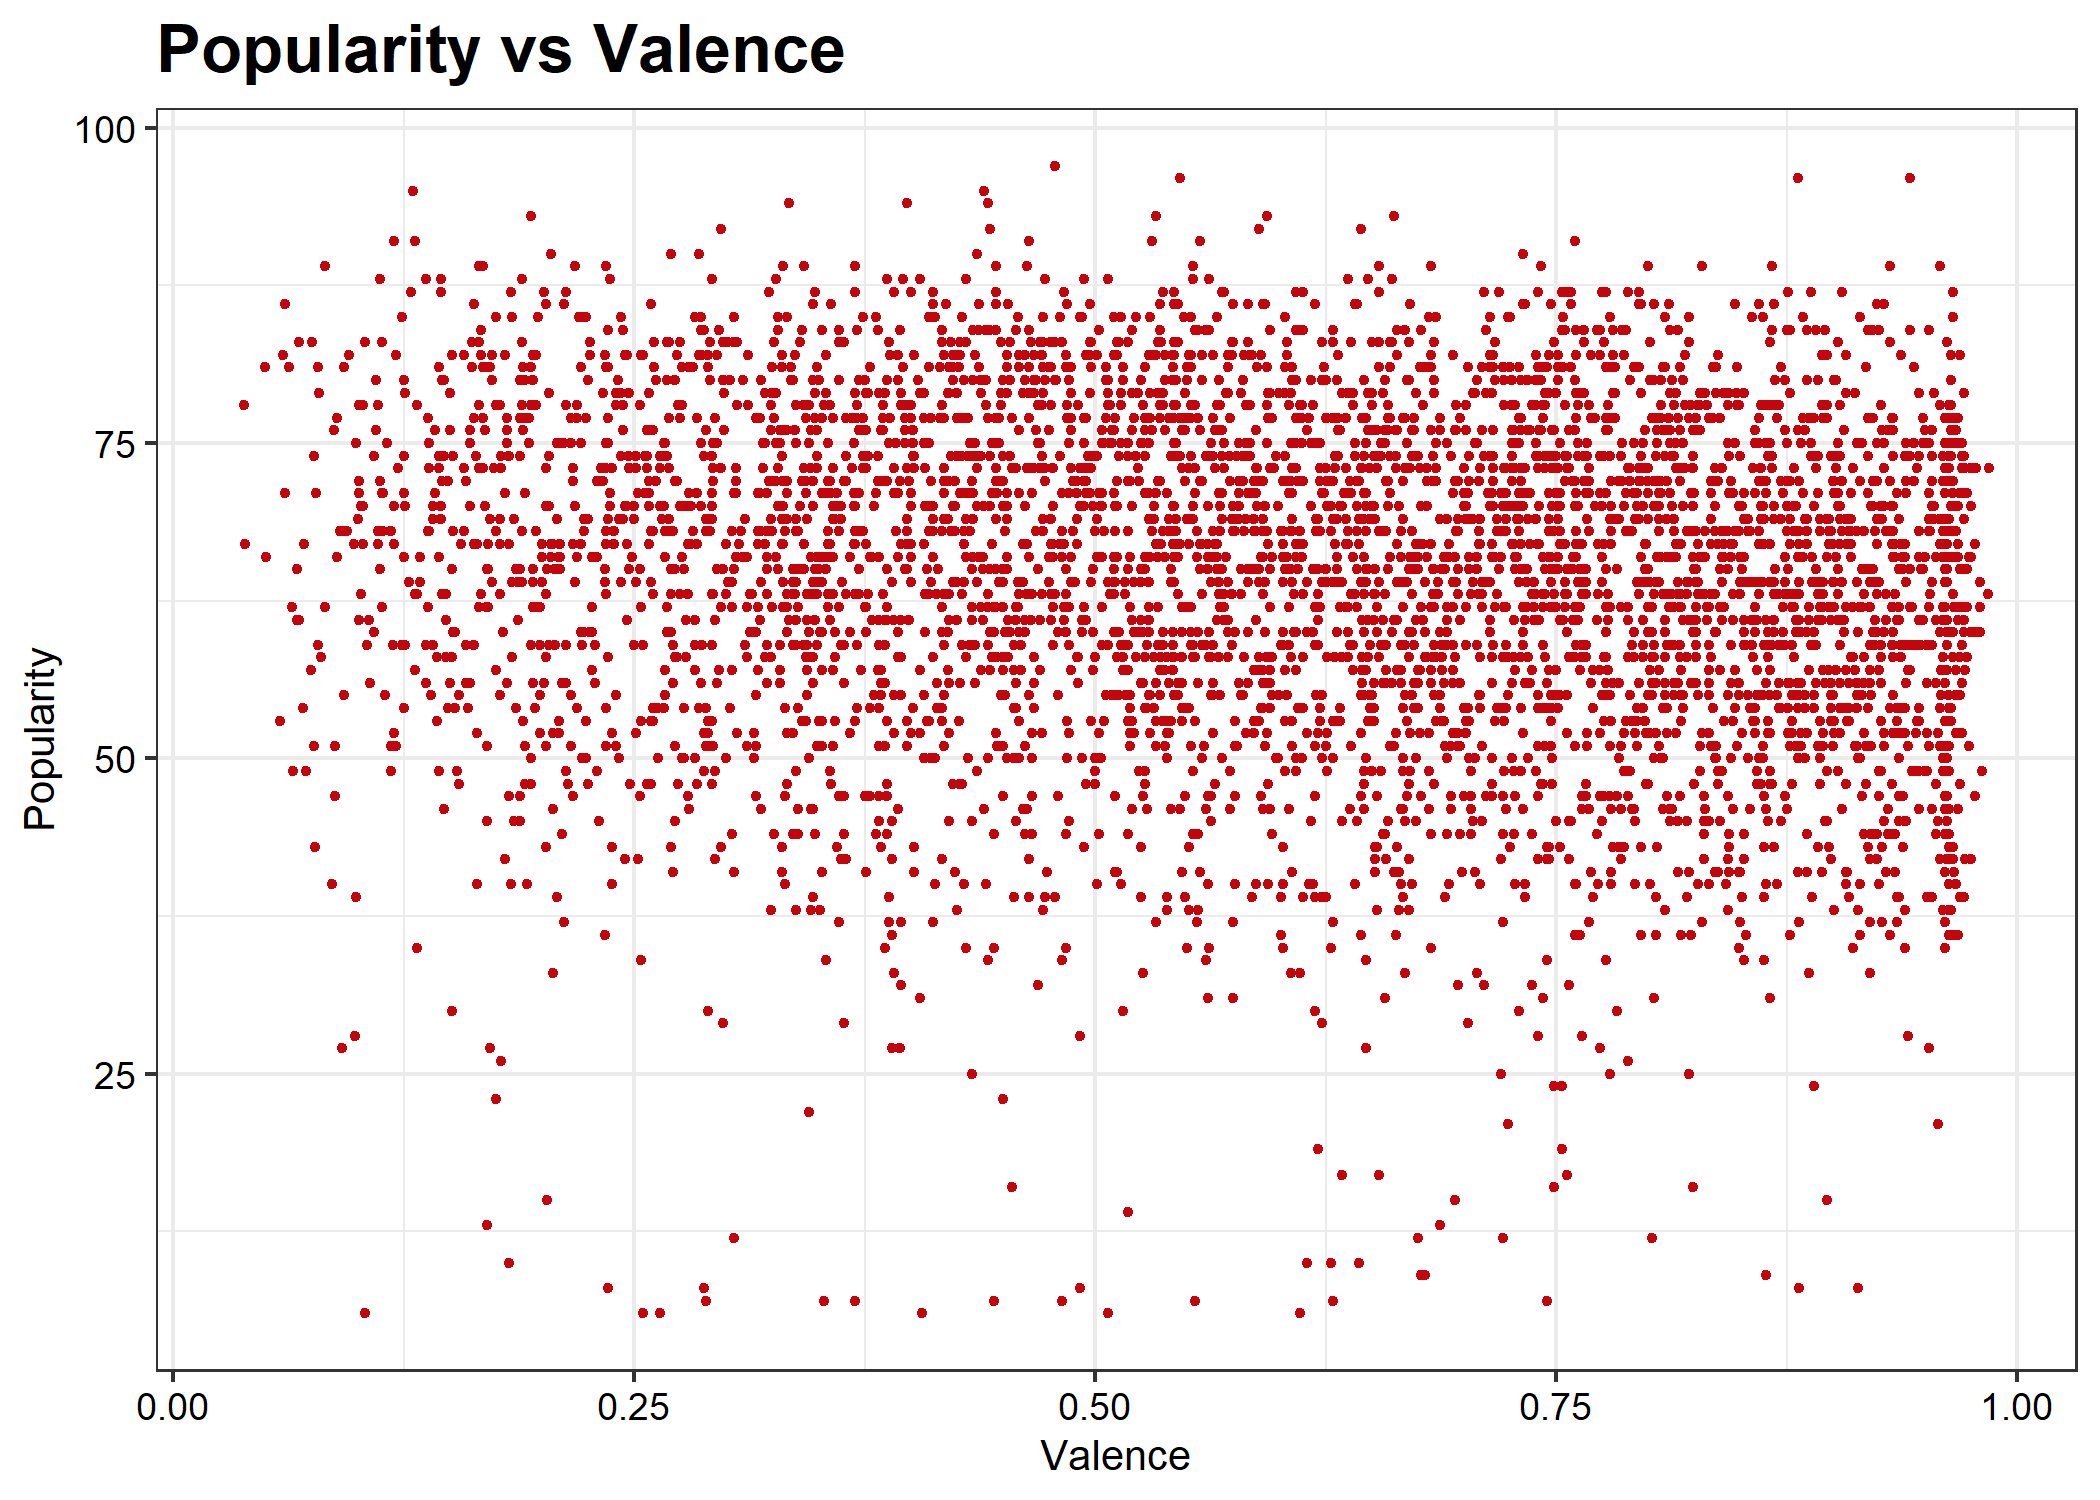
\includegraphics[width = \textwidth]{pop_vs_track_valence.png}
\caption{}
\label{fig:duration_trend}
\end{subfigure}
\caption{Response vs Predictors}
\end{figure}

TODO: brief commentary.

Also need to explain why artist popularity is considered a predictor, since it isn't an audio feature. The idea is that we basically want to control for artist popularity. A super popular artist could put out literally anything and it will be popular regardless of audio features. 

\section{Modeling}

I estimate a standard linear hierarchical model with $J=10$ predictors and $T=6$ decades by which the data are grouped.

$\text{Let } Y_{it} \text{ denote the popularity of song } i \text{ in decade } t$. 

\begin{align*}
Y_{it} \mid \alpha_t \ \beta_{jt} \ \sigma^2 & \sim N(\mu_{it}, \sigma^2) \text{ where } \mu_{it} = \alpha_t + x_i^T\beta_{jt} \\
\alpha_t \mid \mu_\alpha \ \tau_\alpha^2 & \sim N(\mu_{\alpha}, \tau^2_\alpha) \\
\beta_{jt} \mid \mu_{j} \ \tau_{\beta} & \sim N(\mu_{\beta_j}, \tau_\beta^2) \\
\mu_\alpha & \sim N(50, 5) \\
\mu_{\beta_j} & \sim N(\Bar{\mu}_{\beta_{j}}, 1) \\
\tau_\beta^2 & \sim \text{Inv.Gamma}(1.5, 1) \\
\tau_\alpha^2 & \sim \text{Inv.Gamma}(1.5, 1) \\
\sigma^2 & \sim \text{Inv.Gamma}(1.5, 0.3)
\end{align*}

The hyperparameter $\Bar{\mu}_{\beta_{j}}$ were set to reflect a priori beliefs regarding the sign of each coefficient. It was set to $-0.10$ for instrumentalness, acousticness, liveness, and duration, reflecting the belief that the posterior mean for the coefficients associated with these predictors should be negative. For all other predictors, it was set to $0.10$ (since, for instance, we expect the relatiomship between popularity and danceability to be positive). The relatively small absolute value of $0.10$ was chosen so as to not be overly strong. 

TODO: More commentary on the model (e.g., pooled variance for coefficients--variability of the effect of one predictor is essentially the same as the variability of the effect of some other predictor. Means however vary by predictor, since of course the effect of one could differ greater from the effect of another.)

Also TODO: Add some kind of numerical summary of the model. (posterior means of coefficients, MAPE, RMSE, etc.)

Here are some more figures that I intend to include (and comment on). This is all \textit{very} incomplete:

\begin{figure}[H]
\begin{subfigure}[b]{0.5\textwidth}
\centering
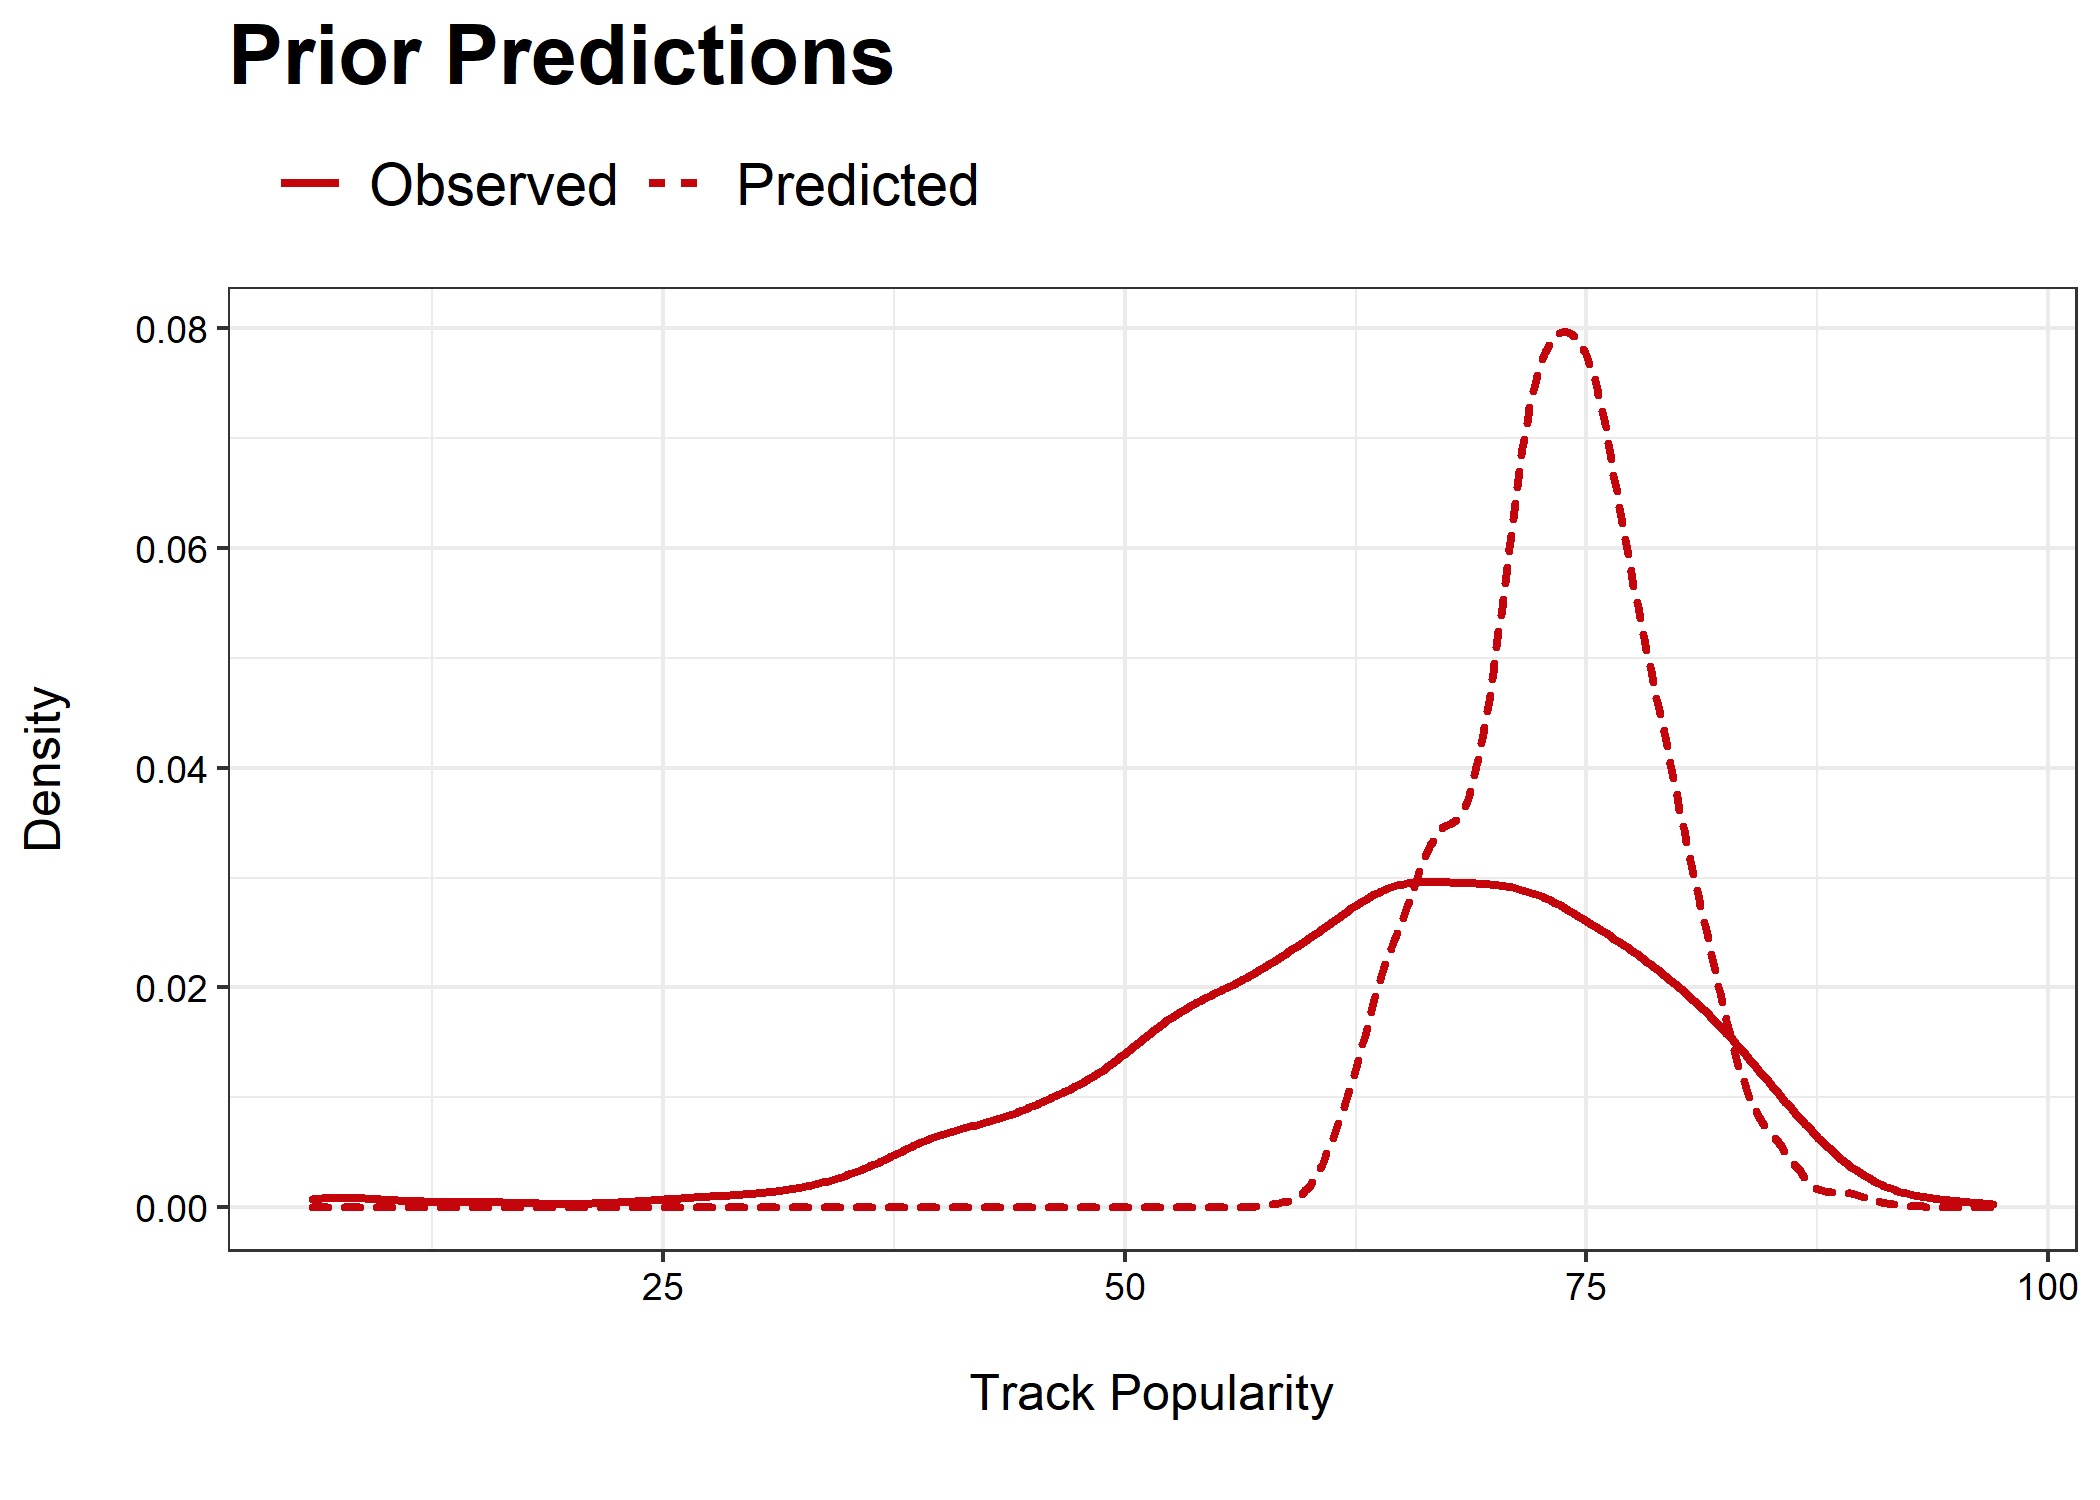
\includegraphics[width = \textwidth]{prior_predictions.png}
\caption{}
\label{fig:prior}
\end{subfigure}
\begin{subfigure}[b]{0.5\textwidth}
\centering
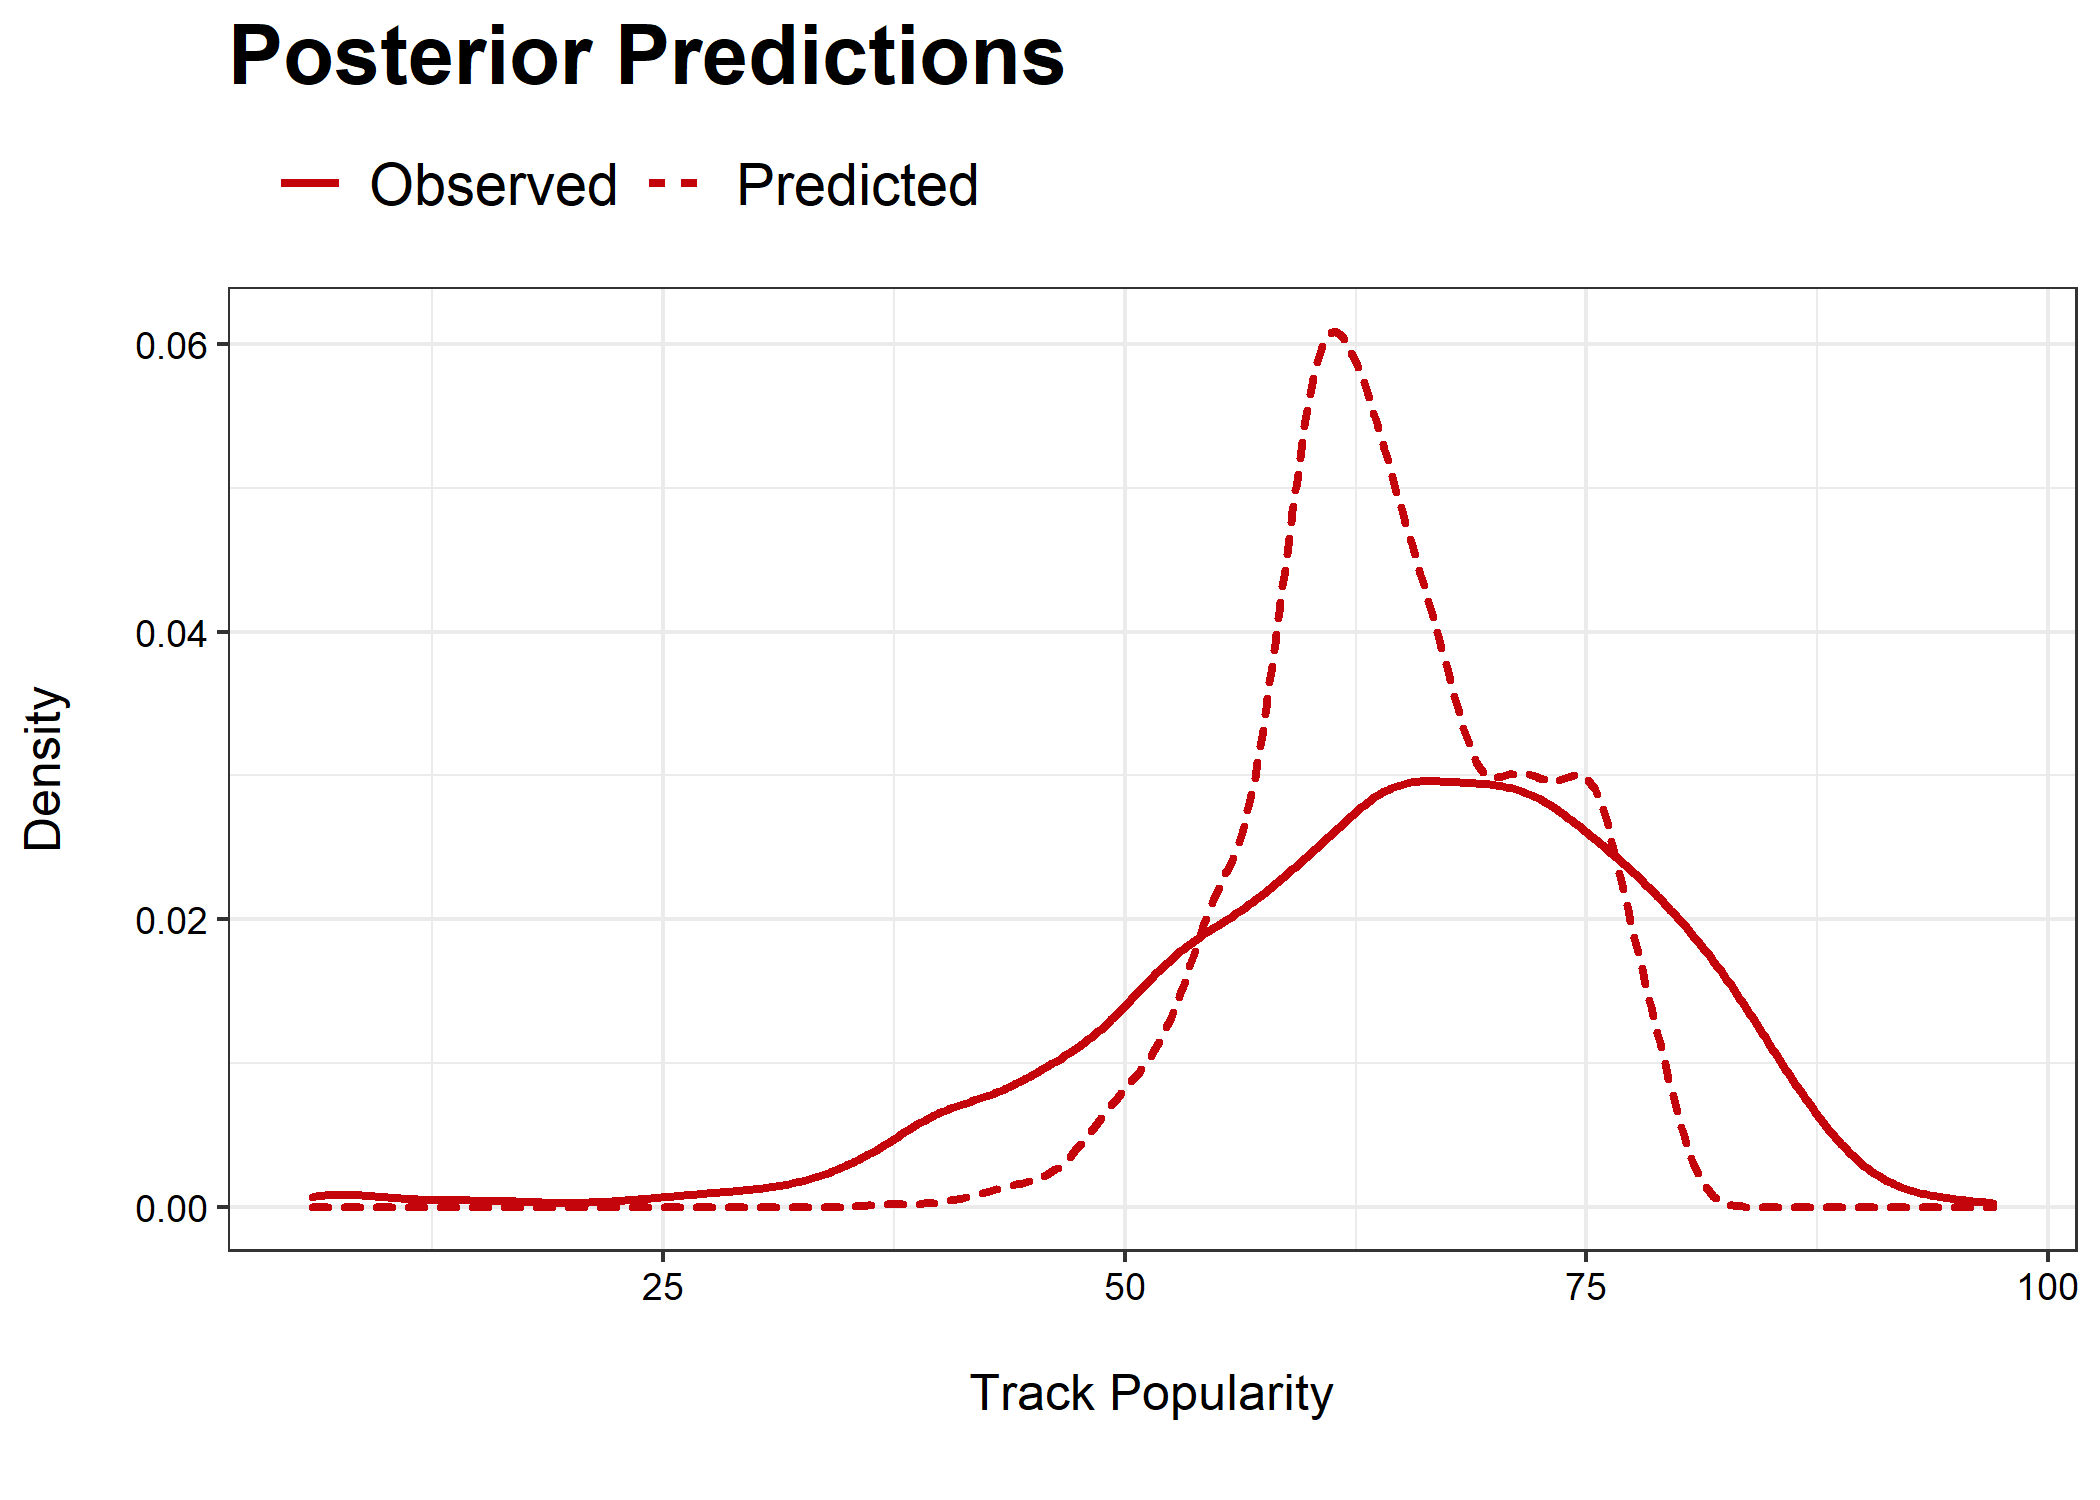
\includegraphics[width = \textwidth]{post_predictions.png}
\caption{}
\label{fig:post}
\end{subfigure}
\caption{Posterior looks pretty bad but it does update the prior reasonably}
\end{figure}
Why's there so much space here ahhh
\begin{figure}[H] % H forces the figure to appear in this location, h! tries really hard to do the same thing
\centering
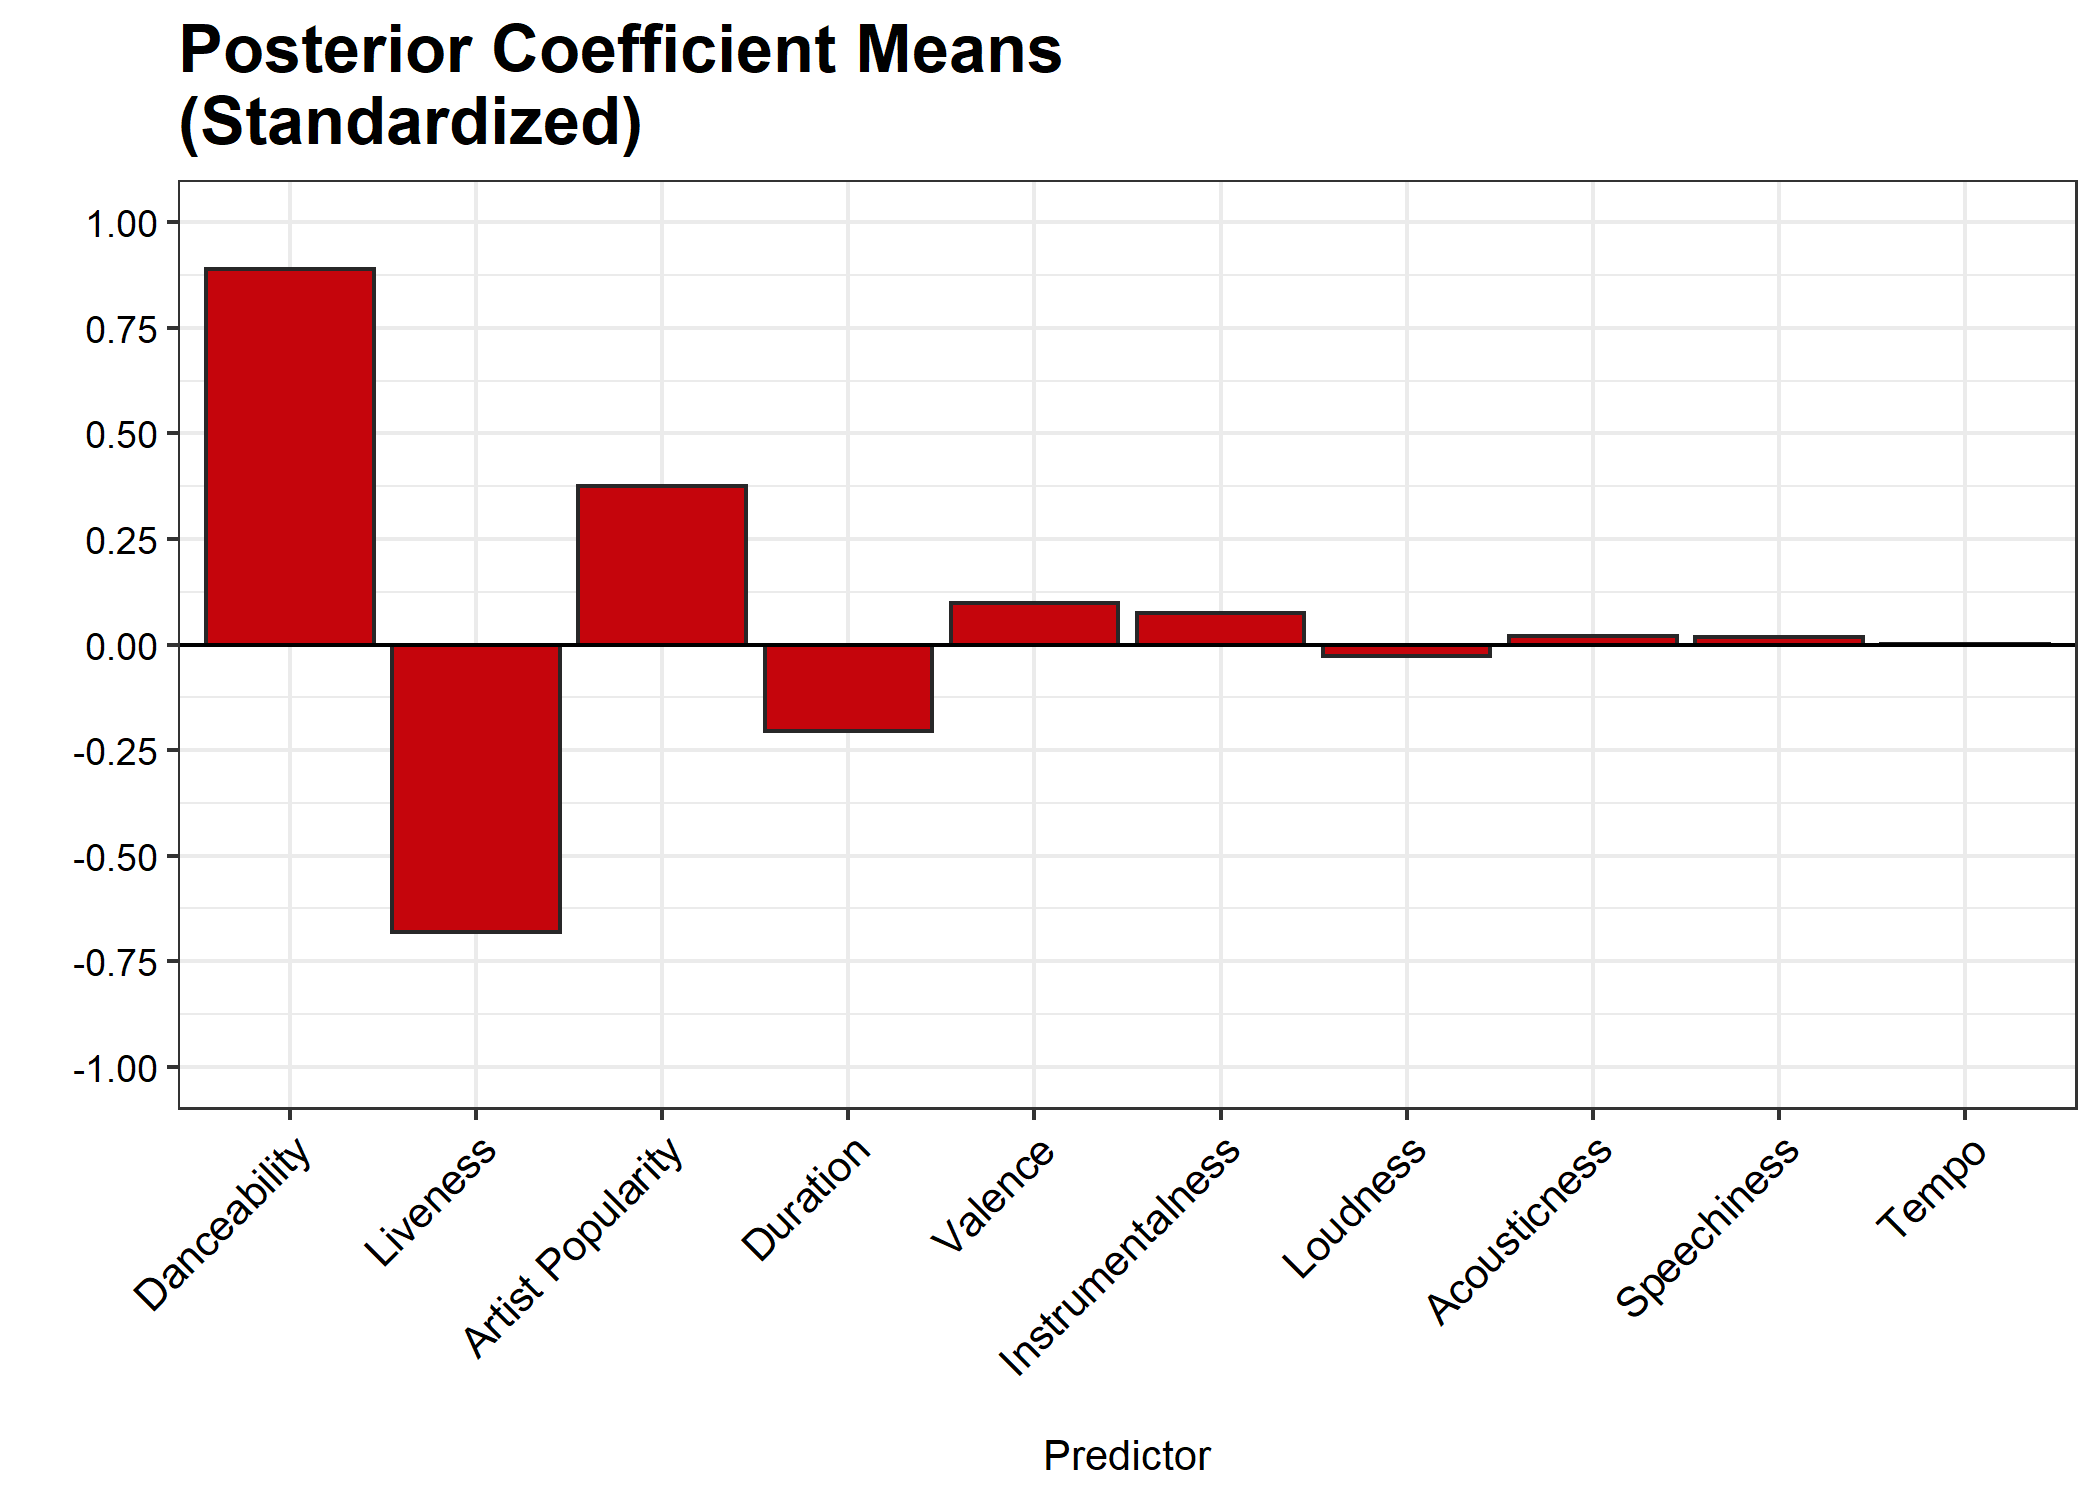
\includegraphics[width=0.7\textwidth]{standardized_coeffs.png} % no need to specify a file extension & pay attention to scaling by width!
\caption{Danceability has largest effect on popularity.}
\label{fig:standardized_coefs} % useful for hyperref'ing later
\end{figure}

\begin{figure}[H] % H forces the figure to appear in this location, h! tries really hard to do the same thing
\centering
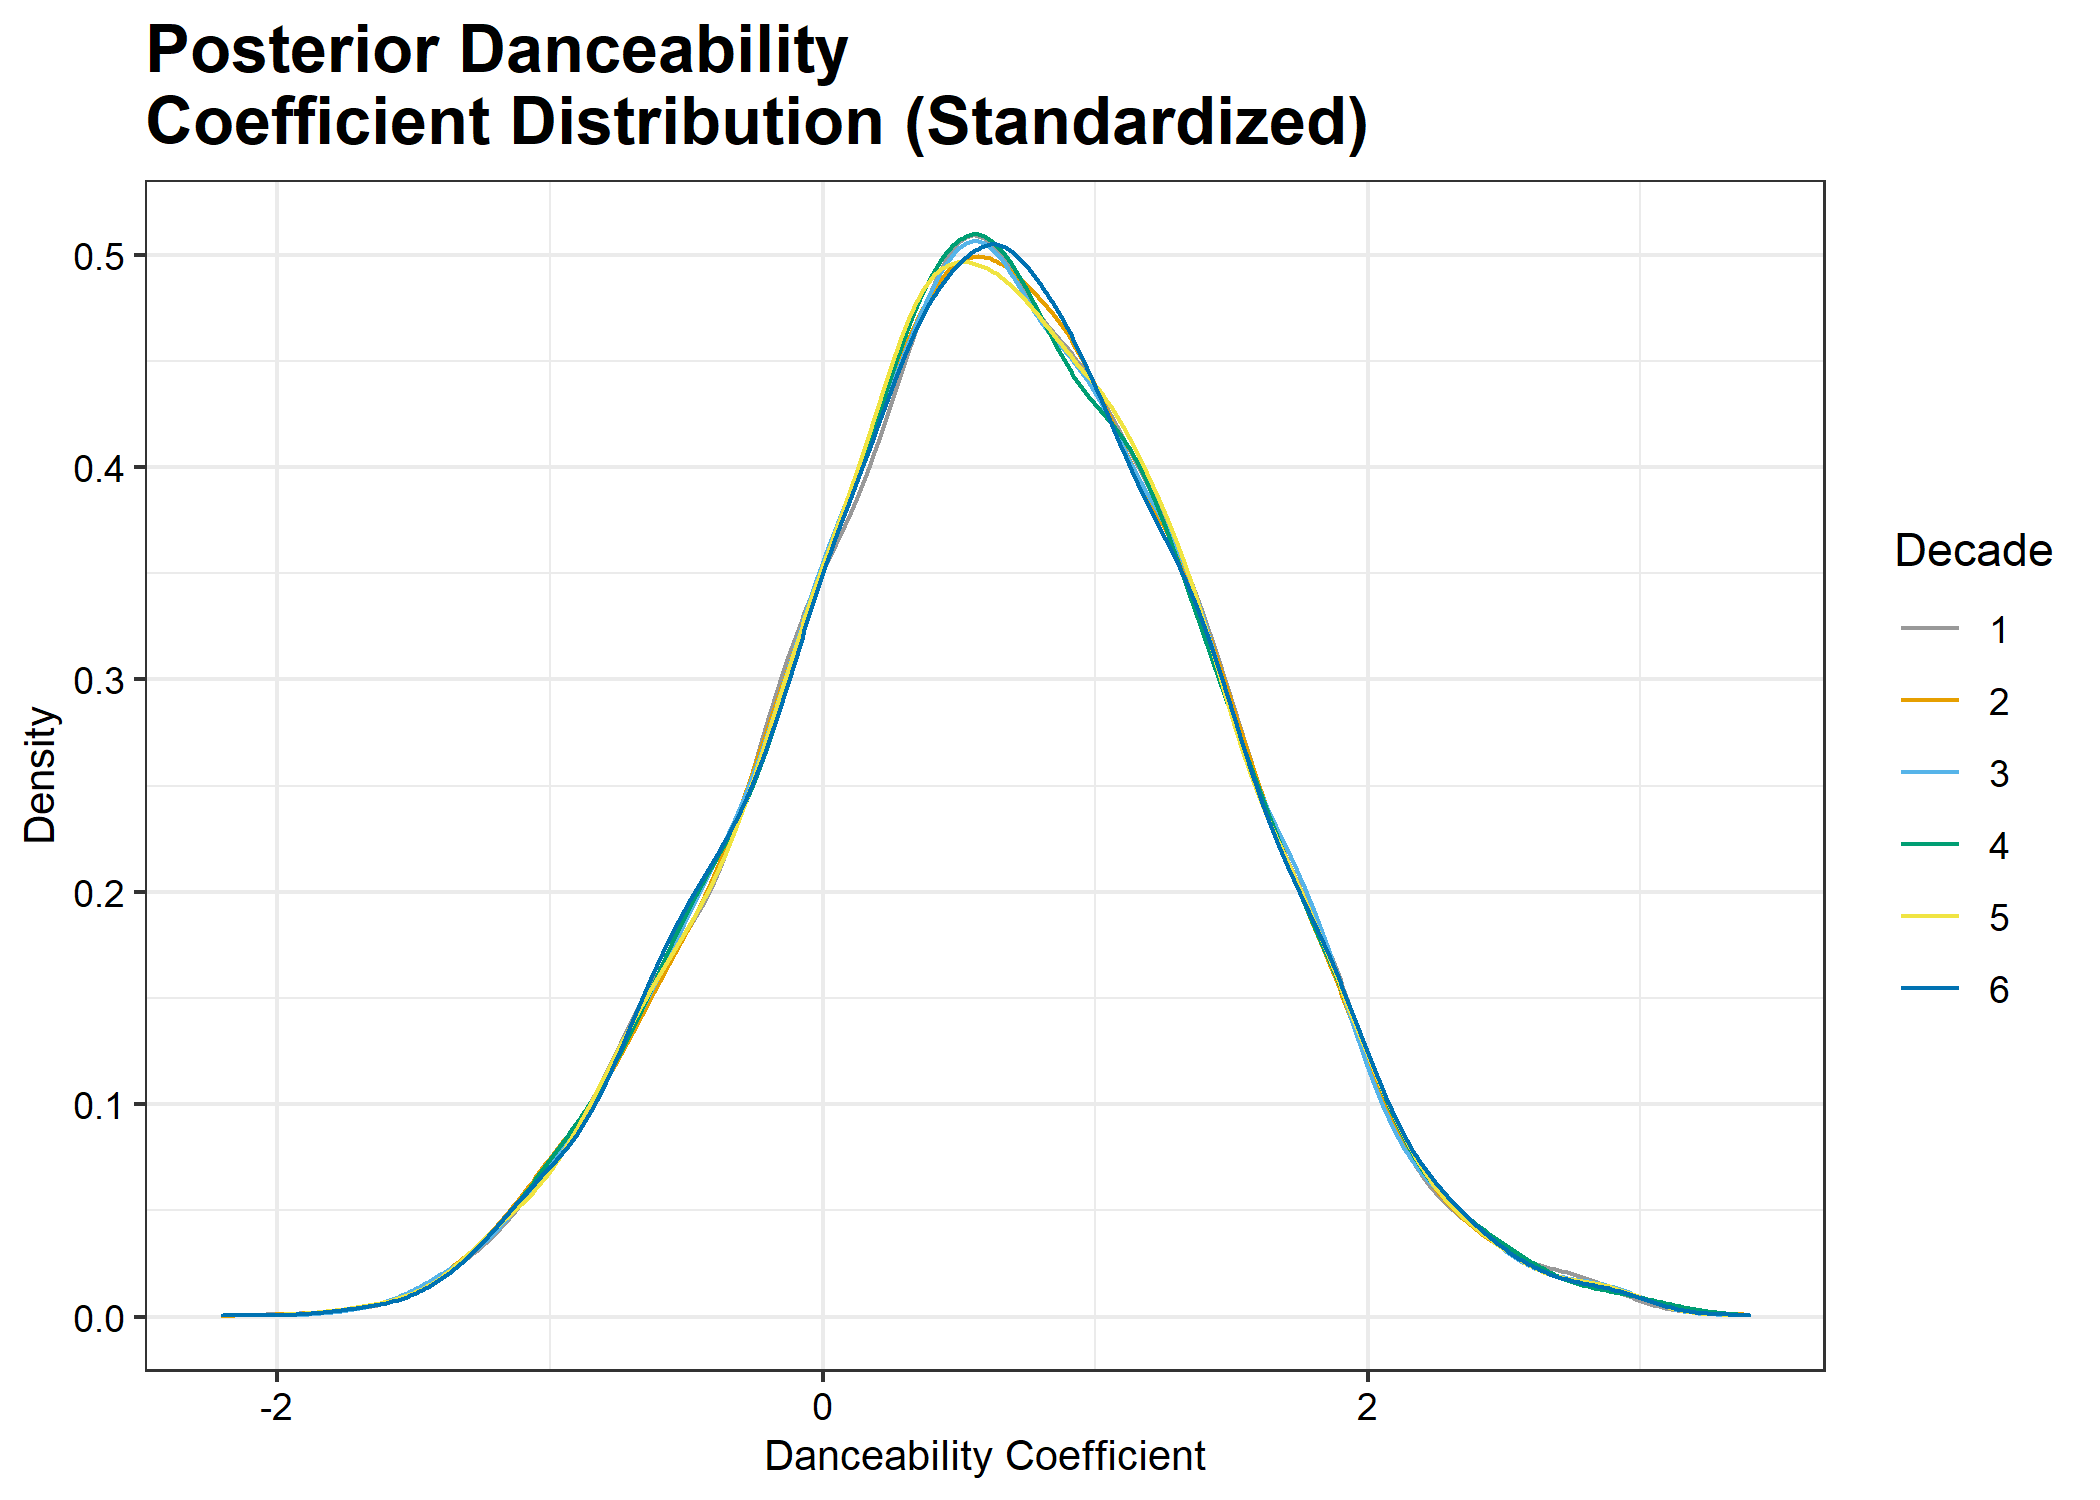
\includegraphics[width=0.7\textwidth]{danceabiltiy_dist.png} % no need to specify a file extension & pay attention to scaling by width!
\caption{Danceability effect not variable across decades (not true for all predictors). We really like dancey songs regardless of decade!}
\label{fig:danceability_dist} % useful for hyperref'ing later
\end{figure}

\begin{figure}[H] % H forces the figure to appear in this location, h! tries really hard to do the same thing
\centering
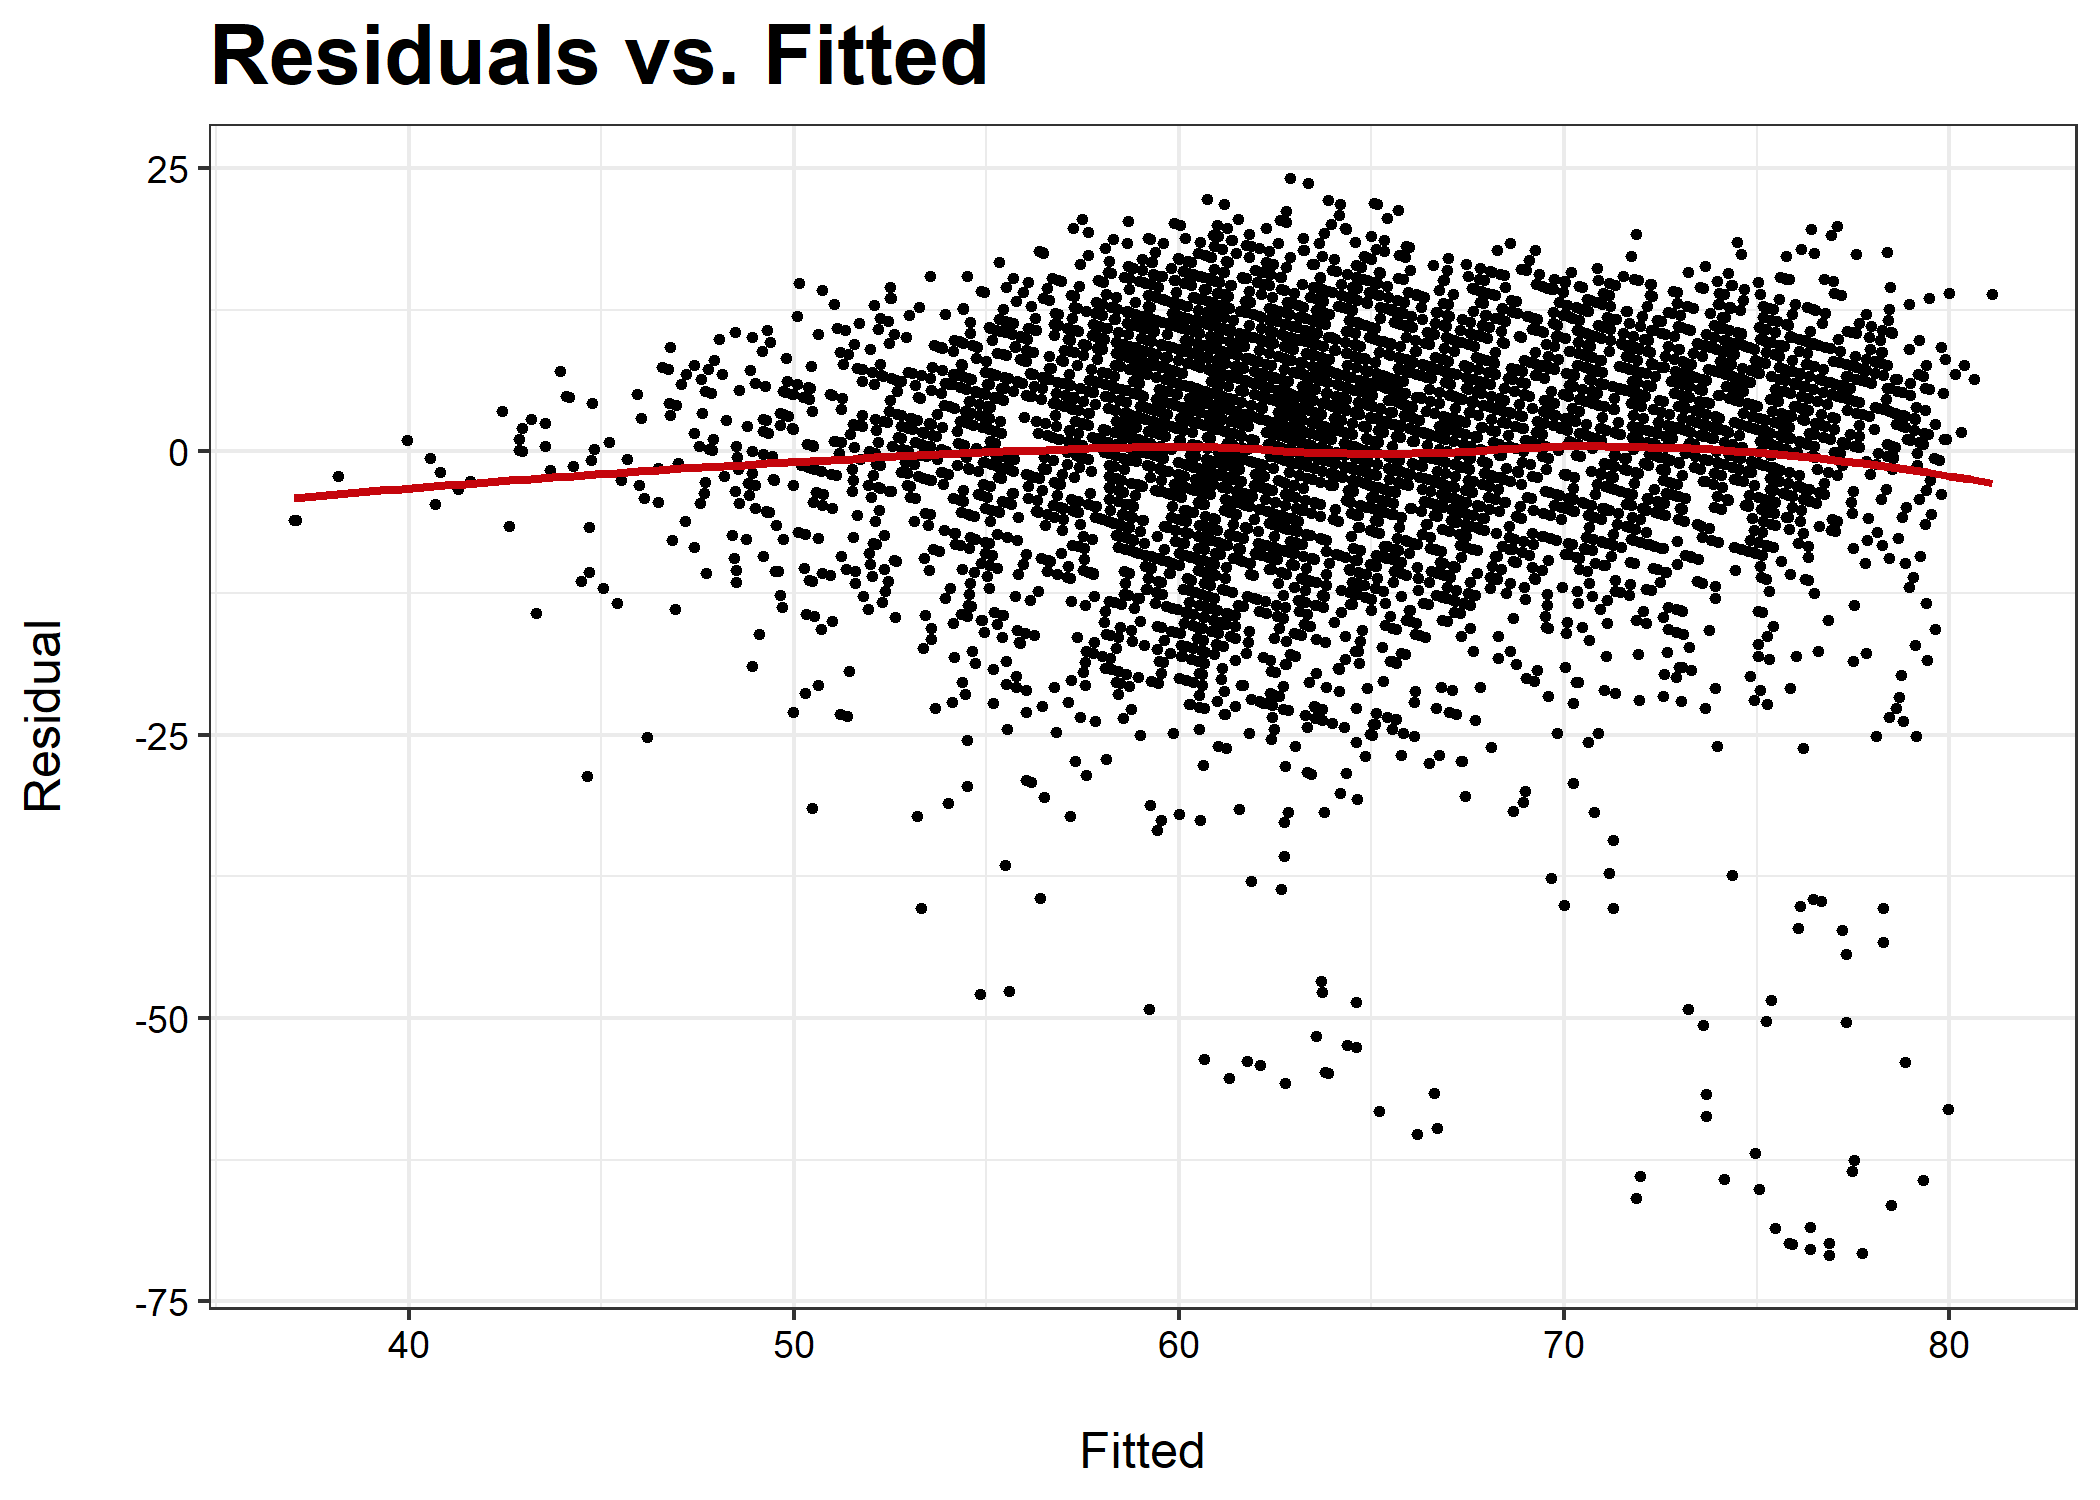
\includegraphics[width=0.7\textwidth]{residuals.png} % no need to specify a file extension & pay attention to scaling by width!
\caption{Probably don't care too much about the residuals, but this shows that there is a systemic problem of predicting low-popularity songs. Have to sympathize with the model a bit, though. Why does "Money For Nothing", a song with hundreds of millions of plays on Spotify, have a popularity score under 10? Also should note that fitted here refers to posterior mean predictions.}
\label{fig:residuals} % useful for hyperref'ing later
\end{figure}

\section{Discussion}

TODO.

% You should conclude your report with a short discussion.
% Immediately following the discussion should be a list of references.
% If you do not already use BibTeX and natbib, now is a great time to learn!
% You should cite any sources using the commands \texttt{citet} for inline references and \texttt{citep} for parenthetical references. 
% So you would use \texttt{citet} to write something like ``\citet{Deshpande2019_mSSL} introduced an EM-like algorithm for simultaneous variable and covariance selection in multi-outcome linear models'' and you would use \texttt{citep} for a sentence like ``Spike-and-slab priors can be effectively deployed to perform simultaneous variable and covariance selection in multi-outcome linear models \citep{Deshpande2019_mSSL}.''

% You should save your references in a \texttt{.bib} file that is located in the same directory as your LaTeX files.

\bibliography{references}


\end{document}
